\documentclass{beamer}
 
\usetheme{default}
\usepackage[latin1]{inputenc}
\usefonttheme{professionalfonts}
\usepackage{times}
\usepackage{pgf,tikz}
\usepackage{amsmath}
\usepackage{verbatim}
\usetikzlibrary{arrows,shapes}
\usepackage{ulem}
\usepackage{longtable}
\usepackage{tabularx}
\usepackage{adjustbox}
\usepackage{multirow}
\usepackage{float}
\usepackage{arydshln}
\usepackage{mathrsfs}




%%% Color
\definecolor{myred}{cmyk}{0, 0.7808, 0.4429, 0.1412}

 
% \usepackage[utf8]{inputenc}
% 
% Bunch of new commands
% 
% brownian motion
\newcommand{\dBm}{dW\left(t\right)}
\newcommand{\dpoiss}{dq\left(t\right)}
\newcommand{\DBm}{\delta{W\left(t\right)}}
\newcommand{\Bm}{W\left(t\right)}
\newcommand{\Bmsub}[1]{W_{#1}\left(t\right)}
\newcommand{\Dt}{\Delta t} 
\newcommand{\Bmdist}{\DBm \sim N \left( 0, \Dt \right)}
\newcommand{\ft}{f\left(t, \Bm \right)}
\newcommand{\E}{\mathop{\mathbb{E}}}
\newcommand{\ct}{c\left(t, x\right)}
\newcommand{\dcx}{\frac{\delta\ct}{\delta x}}
\newcommand{\dciix}{\frac{\delta^2\ct}{\delta x^2}}
\newcommand{\dct}{\frac{\delta\ct}{\delta t}}
\newcommand{\N}[1]{N\left(#1\right)}
\newcommand{\dsub}[1]{d_{#1}\left(\Dt, x\right)}
\newcommand{\call}[2]{c\left( #1, #2\right)}
% % about stock
\newcommand{\St}{S\left(t\right)}
\newcommand{\Vt}{V\left(t\right)}
\newcommand{\Si}{S\left(0\right)}
\newcommand{\dSt}{dS\left(t\right)}
\newcommand{\DSt}{\Delta S\left(t\right)}
\newcommand{\dSr}{\frac{\dSt}{\St}}
\newcommand{\DSr}{\frac{\DSt}{\St}}
\newcommand{\Scontinuous}{\St = \Si e^{\sigma\Bm + \left(\alpha - \frac{1}{2 \sigma^2}\right)t}}
\newcommand{\Itobmdiff}{d\ft = \left[\frac{\partial \ft }{\partial t} + \frac{1}{2} \frac{\partial ^2\ft }{\partial x^2}\right]dt + \frac{\partial \ft}{\partial x} \dBm}
\newcommand{\Scontinousdiff}{d\St &= \alpha \St dt + \sigma \St \dBm}
\newcommand{\Scontinuousrate}{\dSr &= \alpha dt + \sigma \dBm}
 \newcommand{\Sdiscretediff}{d\St &= \alpha \St \Dt + \sigma \St \dBm}
\newcommand{\Sshort}{\Si e^{X}}
\newcommand{\CCRdist}{X \sim N\left(\left(\alpha - \frac{1}{2}\sigma^2\right)t, \sigma^2 t\right)}
\newcommand{\Sdiscreterate}{\DSr &= \alpha \Delta t + \sigma \DBm}
\newcommand{\Sdiscreterateexp}{\E \DSr = \alpha \Dt}
\newcommand{\Sdiscreteratevar}{var \DSr = \sigma ^2 \Dt}
\newcommand{\Sdiscreteratedist}{\DSr \sim N\left(\alpha\Dt, \sigma\Dt\right)}
\newcommand{\Sexp}{\E\St = \Si e^{\alpha t}}
\newcommand{\Svar}{var\St = \Si^2 e^{2\alpha t}\left(e^{\sigma^2 t} - 1\right)}
\newcommand{\Sshortt}{\St = \Si e^{X t}}
\newcommand{\CCRt}{X = \frac{1}{t} \ln{\frac{\St}{\Si}}}
\newcommand{\CCRtdist}{X \sim N\left(\alpha - \frac{\sigma^2}{2}, \frac{\sigma^2}{t}\right)}
\newcommand{\BSMpde}{\dct + r x \dcx + \frac{1}{2} \sigma^2 x^2 \dciix = r\ct}
\newcommand{\BSMeq}[1]{r\call{t}{#1} = \frac{\partial \call{t}{#1}}{\partial t} + r #1 \frac{\partial \call{t}{#1}}{\partial #1} + \frac{1}{2} \sigma ^2 #1 ^2 \frac{\partial ^2 \call{t}{#1}}{\partial #1 ^2}}
\newcommand{\BSMGreeks}[1]{r\call{t}{#1} = \Theta + r #1 \Delta + \frac{1}{2} \sigma ^2 #1 ^2 \Gamma}
\newcommand{\BSMsol}{\ct &= x\N{\dsub{+}} - K e^{-r\Dt} \N{\dsub{-}}}
\newcommand{\dpm}{\dsub{\pm} &= \frac{1}{\sigma\sqrt{\Dt}} \left[\log\frac{x}{K} + \left(r \pm \frac{\sigma^2}{2}\Dt\right)\right]}

% CIR Stock price Stochastic process
\newcommand{\HSVstock}{
  d\St &= \alpha \St dt + \sqrt{\Vt} \St d \Bmsub{S}
}

% CIR Stock price Stochastic process
\newcommand{\HSVstockriskless}{
  d\St &= r \St dt + \sqrt{\Vt} \St d \Bmsub{S}
}

% CIR volatility
\newcommand{\HSVvol}{
  d\Vt &= \kappa\left(\theta - \Vt \right) dt + \sigma \sqrt{\Vt} d \Bmsub{V}
}


% CIR volatility
\newcommand{\HSVvolriskless}{
  d\Vt &= \kappa^{*} \left(\theta^{*} - \Vt \right) dt + \sigma \sqrt{\Vt} d \Bmsub{V}
}

\newcommand{\dportfolio}{dX\left(t\right) = \Delta\left(t\right) d\St + r \left(X\left(t\right) - \Delta\left(t\right) \St \right) dt}
% Snippet
\newcommand{\BSM}{Black--Scholes--Merton }
\newcommand{\lnorm}{log-normally }
\newcommand{\bmotion}{Brownian Motion }
\newcommand{\stvar}{stochastic variable }
\newcommand{\wienpro}{Wiener process }
\newcommand{\markpro}{Markov process }

 
% \usetheme{Boadilla}
% \usecolortheme{default}




%Information to be included in the title page:
\title{Hedging performances of the Black-Scholes model in imperfect log-normal world}
\author{Anthony Tedde}
\institute{Louvain School of Management (LSM)}
\date{2018}
 
 
 
\usepackage{Sweave}
\begin{document}
\Sconcordance{concordance:index.tex:index.Rnw:%
1 6 1}
\Sconcordance{concordance:index.tex:./preamble/usepackage.Rnw:ofs 7:%
1 21 1}
\Sconcordance{concordance:index.tex:./preamble/misc.Rnw:ofs 29:%
1 6 1}
\Sconcordance{concordance:index.tex:./preamble/snippet.Rnw:ofs 36:%
1 7 1}
\Sconcordance{concordance:index.tex:./preamble/formula.Rnw:ofs 44:%
1 71 1}
\Sconcordance{concordance:index.tex:index.Rnw:ofs 116:%
12 1 1 1 0 24 1}
\Sconcordance{concordance:index.tex:./methodology.Rnw:ofs 143:%
1 485 1}
\Sconcordance{concordance:index.tex:index.Rnw:ofs 629:%
39 12 1}

 
%---Table of content---------------------------------------------------------
\frame{\titlepage}
\section[]{}
\begin{frame}{Contents}
  \tableofcontents
\end{frame}
%---Fim do Sumário------------------------------------------------------------





% =============================================================================
% CONTEXT
% =============================================================================
% \SweaveInput{context}

% =============================================================================
% Other Models
% =============================================================================
% \SweaveInput{model}


% =============================================================================
% Methodology
% =============================================================================
\section{Other models}


% ----------------------------------------------------------------------------- 
\begin{frame}{Other models}

\tableofcontents[currentsection]
 
\end{frame}
% -----------------------------------------------------------------------------





\subsection{Merton's Jump-Diffusion Model}
% ----------------------------------------------------------------------------- 
\begin{frame}{The Merton's Jump-Diffusion Model (MJD)}

\begin{block}{MJD stochastic process}
  \begin{align}
  \St &= S\left(0\right) e^{\left(\alpha - \frac{\sigma^2}{2} - \lambda \kappa\right) t + \sigma \Bm + \sum_{i=1}^{N_t} Y_i}
  \notag
\end{align}
  
\end{block}


\begin{block}{Graphical representation}
  \begin{figure}[ht]
  \centering
  % Created by tikzDevice version 0.11 on 2018-08-25 21:52:27
% !TEX encoding = UTF-8 Unicode
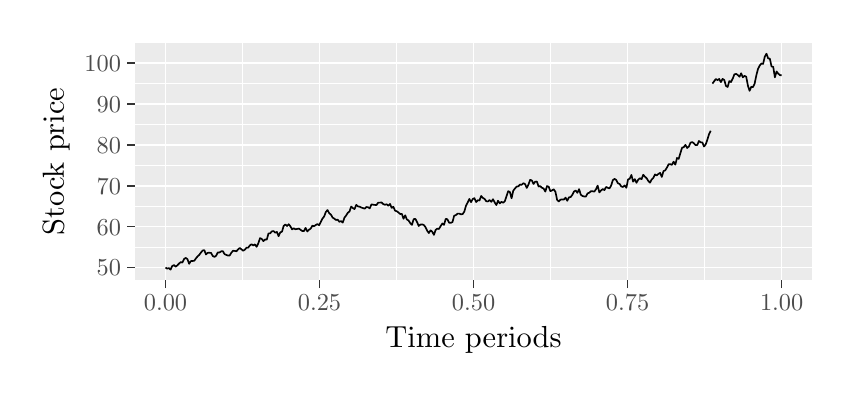
\begin{tikzpicture}[x=1pt,y=1pt]
\definecolor{fillColor}{RGB}{255,255,255}
\path[use as bounding box,fill=fillColor,fill opacity=0.00] (0,0) rectangle (289.08,122.86);
\begin{scope}
\path[clip] (  0.00,  0.00) rectangle (289.08,122.86);
\definecolor{drawColor}{RGB}{255,255,255}
\definecolor{fillColor}{RGB}{255,255,255}

\path[draw=drawColor,line width= 0.6pt,line join=round,line cap=round,fill=fillColor] (  0.00,  0.00) rectangle (289.08,122.86);
\end{scope}
\begin{scope}
\path[clip] ( 38.67, 31.53) rectangle (283.58,117.36);
\definecolor{fillColor}{gray}{0.92}

\path[fill=fillColor] ( 38.67, 31.53) rectangle (283.58,117.36);
\definecolor{drawColor}{RGB}{255,255,255}

\path[draw=drawColor,line width= 0.3pt,line join=round] ( 38.67, 43.58) --
	(283.58, 43.58);

\path[draw=drawColor,line width= 0.3pt,line join=round] ( 38.67, 58.35) --
	(283.58, 58.35);

\path[draw=drawColor,line width= 0.3pt,line join=round] ( 38.67, 73.12) --
	(283.58, 73.12);

\path[draw=drawColor,line width= 0.3pt,line join=round] ( 38.67, 87.89) --
	(283.58, 87.89);

\path[draw=drawColor,line width= 0.3pt,line join=round] ( 38.67,102.66) --
	(283.58,102.66);

\path[draw=drawColor,line width= 0.3pt,line join=round] ( 77.63, 31.53) --
	( 77.63,117.36);

\path[draw=drawColor,line width= 0.3pt,line join=round] (133.29, 31.53) --
	(133.29,117.36);

\path[draw=drawColor,line width= 0.3pt,line join=round] (188.95, 31.53) --
	(188.95,117.36);

\path[draw=drawColor,line width= 0.3pt,line join=round] (244.62, 31.53) --
	(244.62,117.36);

\path[draw=drawColor,line width= 0.6pt,line join=round] ( 38.67, 36.19) --
	(283.58, 36.19);

\path[draw=drawColor,line width= 0.6pt,line join=round] ( 38.67, 50.96) --
	(283.58, 50.96);

\path[draw=drawColor,line width= 0.6pt,line join=round] ( 38.67, 65.73) --
	(283.58, 65.73);

\path[draw=drawColor,line width= 0.6pt,line join=round] ( 38.67, 80.50) --
	(283.58, 80.50);

\path[draw=drawColor,line width= 0.6pt,line join=round] ( 38.67, 95.27) --
	(283.58, 95.27);

\path[draw=drawColor,line width= 0.6pt,line join=round] ( 38.67,110.04) --
	(283.58,110.04);

\path[draw=drawColor,line width= 0.6pt,line join=round] ( 49.80, 31.53) --
	( 49.80,117.36);

\path[draw=drawColor,line width= 0.6pt,line join=round] (105.46, 31.53) --
	(105.46,117.36);

\path[draw=drawColor,line width= 0.6pt,line join=round] (161.12, 31.53) --
	(161.12,117.36);

\path[draw=drawColor,line width= 0.6pt,line join=round] (216.79, 31.53) --
	(216.79,117.36);

\path[draw=drawColor,line width= 0.6pt,line join=round] (272.45, 31.53) --
	(272.45,117.36);
\definecolor{drawColor}{RGB}{0,0,0}

\path[draw=drawColor,line width= 0.6pt,line join=round] ( 49.80, 36.19) --
	( 50.41, 35.78) --
	( 51.02, 36.00) --
	( 51.63, 35.43) --
	( 52.24, 36.74) --
	( 52.85, 37.07) --
	( 53.46, 36.51) --
	( 54.07, 36.96) --
	( 54.68, 37.61) --
	( 55.29, 38.15) --
	( 55.90, 37.98) --
	( 56.51, 39.26) --
	( 57.12, 39.66) --
	( 57.73, 39.23) --
	( 58.34, 37.54) --
	( 58.95, 38.51) --
	( 59.56, 38.55) --
	( 60.17, 38.62) --
	( 60.78, 39.45) --
	( 61.39, 40.20) --
	( 62.00, 40.76) --
	( 62.61, 41.60) --
	( 63.22, 42.33) --
	( 63.83, 42.47) --
	( 64.44, 40.90) --
	( 65.05, 41.49) --
	( 65.66, 41.52) --
	( 66.27, 41.47) --
	( 66.88, 40.34) --
	( 67.49, 40.03) --
	( 68.10, 40.45) --
	( 68.71, 41.65) --
	( 69.32, 41.64) --
	( 69.93, 42.05) --
	( 70.54, 42.08) --
	( 71.15, 41.02) --
	( 71.76, 40.76) --
	( 72.37, 40.51) --
	( 72.98, 40.54) --
	( 73.59, 41.53) --
	( 74.20, 42.24) --
	( 74.81, 42.19) --
	( 75.42, 42.06) --
	( 76.03, 42.72) --
	( 76.64, 43.27) --
	( 77.25, 42.77) --
	( 77.86, 42.26) --
	( 78.47, 42.64) --
	( 79.08, 43.37) --
	( 79.69, 43.36) --
	( 80.30, 44.19) --
	( 80.91, 44.62) --
	( 81.52, 44.17) --
	( 82.13, 44.55) --
	( 82.74, 43.66) --
	( 83.35, 44.98) --
	( 83.96, 46.79) --
	( 84.57, 46.55) --
	( 85.18, 45.72) --
	( 85.79, 46.31) --
	( 86.40, 46.27) --
	( 87.01, 48.49) --
	( 87.62, 48.55) --
	( 88.23, 49.26) --
	( 88.84, 49.37) --
	( 89.45, 48.78) --
	( 90.06, 49.04) --
	( 90.67, 47.50) --
	( 91.28, 48.91) --
	( 91.89, 49.13) --
	( 92.50, 51.22) --
	( 93.11, 51.75) --
	( 93.72, 51.18) --
	( 94.33, 51.84) --
	( 94.94, 51.06) --
	( 95.55, 49.99) --
	( 96.16, 50.35) --
	( 96.77, 50.03) --
	( 97.38, 50.12) --
	( 97.99, 50.27) --
	( 98.60, 49.82) --
	( 99.21, 49.39) --
	( 99.82, 49.35) --
	(100.43, 50.52) --
	(101.04, 49.21) --
	(101.65, 49.84) --
	(102.26, 50.24) --
	(102.87, 51.31) --
	(103.48, 51.11) --
	(104.09, 51.55) --
	(104.70, 51.89) --
	(105.31, 51.47) --
	(105.92, 52.70) --
	(106.53, 53.89) --
	(107.14, 54.66) --
	(107.75, 56.30) --
	(108.36, 56.95) --
	(108.97, 55.78) --
	(109.58, 55.32) --
	(110.19, 54.23) --
	(110.80, 53.86) --
	(111.41, 53.36) --
	(112.02, 53.49) --
	(112.63, 52.72) --
	(113.24, 52.96) --
	(113.85, 52.43) --
	(114.46, 54.21) --
	(115.07, 54.99) --
	(115.68, 55.97) --
	(116.29, 56.44) --
	(116.90, 58.21) --
	(117.51, 57.67) --
	(118.12, 57.31) --
	(118.73, 58.84) --
	(119.34, 58.28) --
	(119.95, 58.17) --
	(120.56, 57.87) --
	(121.17, 57.65) --
	(121.78, 57.47) --
	(122.39, 58.06) --
	(123.00, 57.97) --
	(123.61, 57.56) --
	(124.22, 59.01) --
	(124.83, 58.89) --
	(125.44, 58.81) --
	(126.05, 58.80) --
	(126.66, 59.62) --
	(127.27, 59.64) --
	(127.88, 59.70) --
	(128.49, 59.11) --
	(129.10, 58.88) --
	(129.71, 59.04) --
	(130.32, 58.54) --
	(130.93, 59.17) --
	(131.54, 57.74) --
	(132.15, 58.14) --
	(132.76, 56.71) --
	(133.37, 56.51) --
	(133.98, 56.08) --
	(134.59, 55.54) --
	(135.20, 55.58) --
	(135.81, 53.82) --
	(136.42, 55.05) --
	(137.03, 53.54) --
	(137.64, 53.19) --
	(138.25, 52.22) --
	(138.86, 51.61) --
	(139.47, 53.67) --
	(140.08, 53.78) --
	(140.69, 52.65) --
	(141.30, 51.20) --
	(141.91, 51.71) --
	(142.52, 51.78) --
	(143.13, 51.57) --
	(143.74, 50.80) --
	(144.35, 49.52) --
	(144.96, 48.63) --
	(145.57, 49.63) --
	(146.18, 49.15) --
	(146.79, 47.98) --
	(147.40, 49.76) --
	(148.01, 50.24) --
	(148.62, 50.11) --
	(149.23, 51.18) --
	(149.84, 52.10) --
	(150.45, 51.61) --
	(151.06, 53.78) --
	(151.67, 53.63) --
	(152.28, 52.37) --
	(152.89, 52.33) --
	(153.50, 52.61) --
	(154.11, 54.91) --
	(154.72, 55.11) --
	(155.33, 55.65) --
	(155.94, 55.67) --
	(156.55, 55.43) --
	(157.16, 55.49) --
	(157.77, 56.36) --
	(158.38, 58.52) --
	(158.99, 59.66) --
	(159.60, 60.99) --
	(160.21, 59.83) --
	(160.82, 60.94) --
	(161.43, 61.26) --
	(162.04, 59.85) --
	(162.65, 60.49) --
	(163.26, 60.42) --
	(163.87, 62.04) --
	(164.48, 61.34) --
	(165.09, 61.00) --
	(165.70, 60.14) --
	(166.31, 60.06) --
	(166.92, 60.57) --
	(167.53, 59.92) --
	(168.14, 60.87) --
	(168.75, 59.73) --
	(169.36, 58.76) --
	(169.97, 60.33) --
	(170.58, 59.39) --
	(171.19, 59.91) --
	(171.80, 59.61) --
	(172.41, 60.13) --
	(173.02, 61.97) --
	(173.63, 63.75) --
	(174.24, 63.50) --
	(174.85, 61.20) --
	(175.46, 63.93) --
	(176.07, 64.74) --
	(176.68, 65.43) --
	(177.29, 65.52) --
	(177.90, 66.17) --
	(178.51, 66.10) --
	(179.12, 66.66) --
	(179.73, 66.33) --
	(180.34, 64.95) --
	(180.95, 66.12) --
	(181.56, 67.89) --
	(182.17, 67.66) --
	(182.78, 66.39) --
	(183.39, 67.20) --
	(184.00, 67.25) --
	(184.61, 65.47) --
	(185.22, 65.58) --
	(185.83, 65.00) --
	(186.44, 64.74) --
	(187.05, 63.61) --
	(187.66, 65.64) --
	(188.27, 65.39) --
	(188.88, 63.77) --
	(189.49, 64.08) --
	(190.10, 64.47) --
	(190.71, 63.52) --
	(191.32, 60.60) --
	(191.93, 60.05) --
	(192.54, 60.73) --
	(193.15, 60.77) --
	(193.76, 60.76) --
	(194.37, 61.44) --
	(194.98, 60.32) --
	(195.59, 61.55) --
	(196.20, 61.64) --
	(196.81, 62.48) --
	(197.42, 63.67) --
	(198.03, 64.01) --
	(198.64, 63.18) --
	(199.25, 64.52) --
	(199.86, 62.51) --
	(200.47, 62.04) --
	(201.08, 61.87) --
	(201.69, 61.80) --
	(202.30, 62.97) --
	(202.91, 63.21) --
	(203.52, 63.74) --
	(204.13, 63.77) --
	(204.74, 63.61) --
	(205.35, 64.45) --
	(205.96, 65.79) --
	(206.57, 63.32) --
	(207.18, 64.03) --
	(207.79, 64.53) --
	(208.40, 64.18) --
	(209.01, 65.30) --
	(209.62, 64.99) --
	(210.23, 64.79) --
	(210.84, 65.81) --
	(211.45, 67.80) --
	(212.06, 68.20) --
	(212.67, 67.84) --
	(213.28, 66.64) --
	(213.89, 66.39) --
	(214.50, 65.47) --
	(215.11, 65.30) --
	(215.72, 65.83) --
	(216.33, 65.01) --
	(216.94, 68.00) --
	(217.55, 68.28) --
	(218.16, 69.65) --
	(218.77, 67.22) --
	(219.38, 68.14) --
	(219.99, 66.80) --
	(220.60, 67.91) --
	(221.21, 68.46) --
	(221.82, 68.11) --
	(222.43, 69.70) --
	(223.04, 69.02) --
	(223.65, 68.48) --
	(224.26, 67.48) --
	(224.87, 66.85) --
	(225.48, 68.00) --
	(226.09, 68.59) --
	(226.70, 69.82) --
	(227.31, 69.49) --
	(227.92, 70.02) --
	(228.53, 70.40) --
	(229.14, 68.91) --
	(229.75, 71.02) --
	(230.36, 71.28) --
	(230.97, 72.27) --
	(231.58, 73.49) --
	(232.19, 73.54) --
	(232.80, 73.29) --
	(233.41, 74.45) --
	(234.02, 73.34) --
	(234.63, 75.77) --
	(235.24, 75.43) --
	(235.85, 77.52) --
	(236.46, 79.47) --
	(237.07, 79.69) --
	(237.68, 80.51) --
	(238.29, 79.37) --
	(238.90, 79.88) --
	(239.51, 81.29) --
	(240.12, 81.54) --
	(240.73, 81.09) --
	(241.34, 80.40) --
	(241.95, 80.47) --
	(242.56, 81.92) --
	(243.17, 81.44) --
	(243.78, 81.40) --
	(244.39, 79.92) --
	(245.00, 80.65) --
	(245.61, 82.40) --
	(246.22, 84.42) --
	(246.83, 85.59);

\path[draw=drawColor,line width= 0.6pt,line join=round] (247.44,102.64) --
	(248.05,103.49) --
	(248.66,104.30) --
	(249.27,103.92) --
	(249.88,104.32) --
	(250.49,103.18) --
	(251.10,104.33) --
	(251.71,103.99) --
	(252.32,101.82) --
	(252.93,101.42) --
	(253.54,103.57) --
	(254.15,103.21) --
	(254.76,104.44) --
	(255.37,106.00) --
	(255.98,106.15) --
	(256.59,105.77) --
	(257.20,105.12) --
	(257.81,106.37) --
	(258.42,104.92) --
	(259.03,105.43) --
	(259.64,105.14) --
	(260.25,101.94) --
	(260.86,100.03) --
	(261.47,101.50) --
	(262.08,101.36) --
	(262.69,102.67) --
	(263.30,105.62) --
	(263.91,107.99) --
	(264.52,109.18) --
	(265.13,109.91) --
	(265.74,109.76) --
	(266.35,112.37) --
	(266.96,113.46) --
	(267.57,111.76) --
	(268.18,111.67) --
	(268.79,108.85) --
	(269.40,108.69) --
	(270.01,104.92) --
	(270.62,107.04) --
	(271.23,106.23) --
	(271.84,105.72) --
	(272.45,105.61);
\end{scope}
\begin{scope}
\path[clip] (  0.00,  0.00) rectangle (289.08,122.86);
\definecolor{drawColor}{gray}{0.30}

\node[text=drawColor,anchor=base east,inner sep=0pt, outer sep=0pt, scale=  0.88] at ( 33.72, 33.16) {50};

\node[text=drawColor,anchor=base east,inner sep=0pt, outer sep=0pt, scale=  0.88] at ( 33.72, 47.93) {60};

\node[text=drawColor,anchor=base east,inner sep=0pt, outer sep=0pt, scale=  0.88] at ( 33.72, 62.70) {70};

\node[text=drawColor,anchor=base east,inner sep=0pt, outer sep=0pt, scale=  0.88] at ( 33.72, 77.47) {80};

\node[text=drawColor,anchor=base east,inner sep=0pt, outer sep=0pt, scale=  0.88] at ( 33.72, 92.24) {90};

\node[text=drawColor,anchor=base east,inner sep=0pt, outer sep=0pt, scale=  0.88] at ( 33.72,107.01) {100};
\end{scope}
\begin{scope}
\path[clip] (  0.00,  0.00) rectangle (289.08,122.86);
\definecolor{drawColor}{gray}{0.20}

\path[draw=drawColor,line width= 0.6pt,line join=round] ( 35.92, 36.19) --
	( 38.67, 36.19);

\path[draw=drawColor,line width= 0.6pt,line join=round] ( 35.92, 50.96) --
	( 38.67, 50.96);

\path[draw=drawColor,line width= 0.6pt,line join=round] ( 35.92, 65.73) --
	( 38.67, 65.73);

\path[draw=drawColor,line width= 0.6pt,line join=round] ( 35.92, 80.50) --
	( 38.67, 80.50);

\path[draw=drawColor,line width= 0.6pt,line join=round] ( 35.92, 95.27) --
	( 38.67, 95.27);

\path[draw=drawColor,line width= 0.6pt,line join=round] ( 35.92,110.04) --
	( 38.67,110.04);
\end{scope}
\begin{scope}
\path[clip] (  0.00,  0.00) rectangle (289.08,122.86);
\definecolor{drawColor}{gray}{0.20}

\path[draw=drawColor,line width= 0.6pt,line join=round] ( 49.80, 28.78) --
	( 49.80, 31.53);

\path[draw=drawColor,line width= 0.6pt,line join=round] (105.46, 28.78) --
	(105.46, 31.53);

\path[draw=drawColor,line width= 0.6pt,line join=round] (161.12, 28.78) --
	(161.12, 31.53);

\path[draw=drawColor,line width= 0.6pt,line join=round] (216.79, 28.78) --
	(216.79, 31.53);

\path[draw=drawColor,line width= 0.6pt,line join=round] (272.45, 28.78) --
	(272.45, 31.53);
\end{scope}
\begin{scope}
\path[clip] (  0.00,  0.00) rectangle (289.08,122.86);
\definecolor{drawColor}{gray}{0.30}

\node[text=drawColor,anchor=base,inner sep=0pt, outer sep=0pt, scale=  0.88] at ( 49.80, 20.52) {0.00};

\node[text=drawColor,anchor=base,inner sep=0pt, outer sep=0pt, scale=  0.88] at (105.46, 20.52) {0.25};

\node[text=drawColor,anchor=base,inner sep=0pt, outer sep=0pt, scale=  0.88] at (161.12, 20.52) {0.50};

\node[text=drawColor,anchor=base,inner sep=0pt, outer sep=0pt, scale=  0.88] at (216.79, 20.52) {0.75};

\node[text=drawColor,anchor=base,inner sep=0pt, outer sep=0pt, scale=  0.88] at (272.45, 20.52) {1.00};
\end{scope}
\begin{scope}
\path[clip] (  0.00,  0.00) rectangle (289.08,122.86);
\definecolor{drawColor}{RGB}{0,0,0}

\node[text=drawColor,anchor=base,inner sep=0pt, outer sep=0pt, scale=  1.10] at (161.12,  7.44) {Time periods};
\end{scope}
\begin{scope}
\path[clip] (  0.00,  0.00) rectangle (289.08,122.86);
\definecolor{drawColor}{RGB}{0,0,0}

\node[text=drawColor,rotate= 90.00,anchor=base,inner sep=0pt, outer sep=0pt, scale=  1.10] at ( 13.08, 74.44) {Stock price};
\end{scope}
\end{tikzpicture}
 
\end{figure}
  
\end{block}
 
\end{frame}
% -----------------------------------------------------------------------------


% -----------------------------------------------------------------------------
\begin{frame}{MJD: log-return density}

\begin{block}{Impact on the skewness}
\begin{figure}[h]
\centering
% Created by tikzDevice version 0.11 on 2018-08-25 22:08:37
% !TEX encoding = UTF-8 Unicode
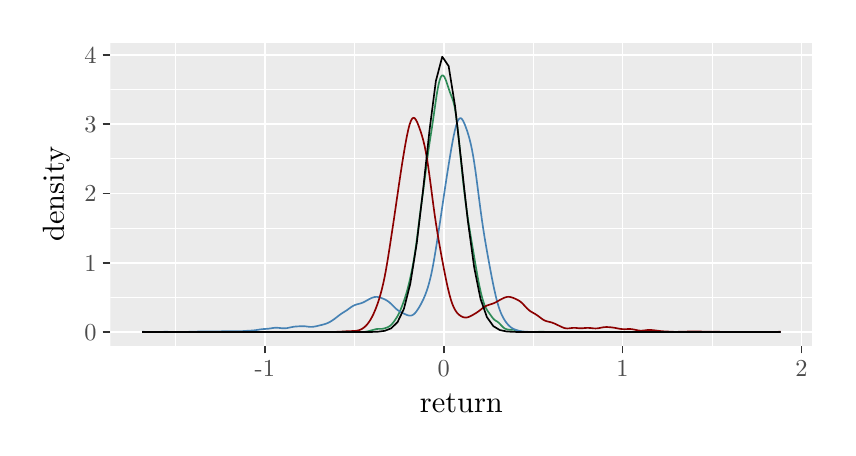
\begin{tikzpicture}[x=1pt,y=1pt]
\definecolor{fillColor}{RGB}{255,255,255}
\path[use as bounding box,fill=fillColor,fill opacity=0.00] (0,0) rectangle (289.08,144.54);
\begin{scope}
\path[clip] (  0.00,  0.00) rectangle (289.08,144.54);
\definecolor{drawColor}{RGB}{255,255,255}
\definecolor{fillColor}{RGB}{255,255,255}

\path[draw=drawColor,line width= 0.6pt,line join=round,line cap=round,fill=fillColor] (  0.00,  0.00) rectangle (289.08,144.54);
\end{scope}
\begin{scope}
\path[clip] ( 29.87, 29.59) rectangle (283.58,139.04);
\definecolor{fillColor}{gray}{0.92}

\path[fill=fillColor] ( 29.87, 29.59) rectangle (283.58,139.04);
\definecolor{drawColor}{RGB}{255,255,255}

\path[draw=drawColor,line width= 0.3pt,line join=round] ( 29.87, 47.07) --
	(283.58, 47.07);

\path[draw=drawColor,line width= 0.3pt,line join=round] ( 29.87, 72.10) --
	(283.58, 72.10);

\path[draw=drawColor,line width= 0.3pt,line join=round] ( 29.87, 97.12) --
	(283.58, 97.12);

\path[draw=drawColor,line width= 0.3pt,line join=round] ( 29.87,122.15) --
	(283.58,122.15);

\path[draw=drawColor,line width= 0.3pt,line join=round] ( 53.40, 29.59) --
	( 53.40,139.04);

\path[draw=drawColor,line width= 0.3pt,line join=round] (118.02, 29.59) --
	(118.02,139.04);

\path[draw=drawColor,line width= 0.3pt,line join=round] (182.64, 29.59) --
	(182.64,139.04);

\path[draw=drawColor,line width= 0.3pt,line join=round] (247.26, 29.59) --
	(247.26,139.04);

\path[draw=drawColor,line width= 0.6pt,line join=round] ( 29.87, 34.56) --
	(283.58, 34.56);

\path[draw=drawColor,line width= 0.6pt,line join=round] ( 29.87, 59.59) --
	(283.58, 59.59);

\path[draw=drawColor,line width= 0.6pt,line join=round] ( 29.87, 84.61) --
	(283.58, 84.61);

\path[draw=drawColor,line width= 0.6pt,line join=round] ( 29.87,109.63) --
	(283.58,109.63);

\path[draw=drawColor,line width= 0.6pt,line join=round] ( 29.87,134.66) --
	(283.58,134.66);

\path[draw=drawColor,line width= 0.6pt,line join=round] ( 85.71, 29.59) --
	( 85.71,139.04);

\path[draw=drawColor,line width= 0.6pt,line join=round] (150.33, 29.59) --
	(150.33,139.04);

\path[draw=drawColor,line width= 0.6pt,line join=round] (214.95, 29.59) --
	(214.95,139.04);

\path[draw=drawColor,line width= 0.6pt,line join=round] (279.57, 29.59) --
	(279.57,139.04);
\definecolor{drawColor}{RGB}{46,139,87}

\path[draw=drawColor,line width= 0.6pt,line join=round] ( 41.40, 34.56) --
	( 41.85, 34.56) --
	( 42.30, 34.56) --
	( 42.76, 34.56) --
	( 43.21, 34.56) --
	( 43.66, 34.56) --
	( 44.11, 34.56) --
	( 44.56, 34.56) --
	( 45.01, 34.56) --
	( 45.46, 34.56) --
	( 45.91, 34.56) --
	( 46.37, 34.56) --
	( 46.82, 34.56) --
	( 47.27, 34.56) --
	( 47.72, 34.56) --
	( 48.17, 34.56) --
	( 48.62, 34.56) --
	( 49.07, 34.56) --
	( 49.53, 34.56) --
	( 49.98, 34.56) --
	( 50.43, 34.56) --
	( 50.88, 34.56) --
	( 51.33, 34.56) --
	( 51.78, 34.56) --
	( 52.23, 34.56) --
	( 52.69, 34.56) --
	( 53.14, 34.56) --
	( 53.59, 34.56) --
	( 54.04, 34.56) --
	( 54.49, 34.56) --
	( 54.94, 34.56) --
	( 55.39, 34.56) --
	( 55.84, 34.56) --
	( 56.30, 34.56) --
	( 56.75, 34.56) --
	( 57.20, 34.56) --
	( 57.65, 34.56) --
	( 58.10, 34.56) --
	( 58.55, 34.56) --
	( 59.00, 34.56) --
	( 59.46, 34.56) --
	( 59.91, 34.56) --
	( 60.36, 34.56) --
	( 60.81, 34.56) --
	( 61.26, 34.56) --
	( 61.71, 34.56) --
	( 62.16, 34.56) --
	( 62.62, 34.56) --
	( 63.07, 34.56) --
	( 63.52, 34.56) --
	( 63.97, 34.56) --
	( 64.42, 34.56) --
	( 64.87, 34.56) --
	( 65.32, 34.56) --
	( 65.77, 34.56) --
	( 66.23, 34.56) --
	( 66.68, 34.56) --
	( 67.13, 34.56) --
	( 67.58, 34.56) --
	( 68.03, 34.56) --
	( 68.48, 34.56) --
	( 68.93, 34.56) --
	( 69.39, 34.56) --
	( 69.84, 34.56) --
	( 70.29, 34.56) --
	( 70.74, 34.56) --
	( 71.19, 34.56) --
	( 71.64, 34.56) --
	( 72.09, 34.56) --
	( 72.55, 34.56) --
	( 73.00, 34.56) --
	( 73.45, 34.56) --
	( 73.90, 34.56) --
	( 74.35, 34.56) --
	( 74.80, 34.56) --
	( 75.25, 34.56) --
	( 75.70, 34.56) --
	( 76.16, 34.56) --
	( 76.61, 34.56) --
	( 77.06, 34.56) --
	( 77.51, 34.56) --
	( 77.96, 34.56) --
	( 78.41, 34.56) --
	( 78.86, 34.56) --
	( 79.32, 34.56) --
	( 79.77, 34.56) --
	( 80.22, 34.56) --
	( 80.67, 34.56) --
	( 81.12, 34.56) --
	( 81.57, 34.56) --
	( 82.02, 34.56) --
	( 82.48, 34.56) --
	( 82.93, 34.56) --
	( 83.38, 34.56) --
	( 83.83, 34.56) --
	( 84.28, 34.56) --
	( 84.73, 34.56) --
	( 85.18, 34.56) --
	( 85.63, 34.56) --
	( 86.09, 34.56) --
	( 86.54, 34.56) --
	( 86.99, 34.56) --
	( 87.44, 34.56) --
	( 87.89, 34.56) --
	( 88.34, 34.56) --
	( 88.79, 34.56) --
	( 89.25, 34.56) --
	( 89.70, 34.56) --
	( 90.15, 34.56) --
	( 90.60, 34.56) --
	( 91.05, 34.56) --
	( 91.50, 34.56) --
	( 91.95, 34.56) --
	( 92.41, 34.56) --
	( 92.86, 34.56) --
	( 93.31, 34.56) --
	( 93.76, 34.56) --
	( 94.21, 34.56) --
	( 94.66, 34.56) --
	( 95.11, 34.56) --
	( 95.56, 34.56) --
	( 96.02, 34.56) --
	( 96.47, 34.56) --
	( 96.92, 34.56) --
	( 97.37, 34.56) --
	( 97.82, 34.56) --
	( 98.27, 34.56) --
	( 98.72, 34.56) --
	( 99.18, 34.56) --
	( 99.63, 34.56) --
	(100.08, 34.56) --
	(100.53, 34.56) --
	(100.98, 34.56) --
	(101.43, 34.56) --
	(101.88, 34.56) --
	(102.34, 34.56) --
	(102.79, 34.56) --
	(103.24, 34.56) --
	(103.69, 34.56) --
	(104.14, 34.56) --
	(104.59, 34.56) --
	(105.04, 34.56) --
	(105.49, 34.56) --
	(105.95, 34.56) --
	(106.40, 34.56) --
	(106.85, 34.56) --
	(107.30, 34.56) --
	(107.75, 34.56) --
	(108.20, 34.56) --
	(108.65, 34.56) --
	(109.11, 34.56) --
	(109.56, 34.56) --
	(110.01, 34.56) --
	(110.46, 34.56) --
	(110.91, 34.56) --
	(111.36, 34.56) --
	(111.81, 34.57) --
	(112.27, 34.57) --
	(112.72, 34.59) --
	(113.17, 34.61) --
	(113.62, 34.63) --
	(114.07, 34.66) --
	(114.52, 34.67) --
	(114.97, 34.67) --
	(115.42, 34.65) --
	(115.88, 34.63) --
	(116.33, 34.60) --
	(116.78, 34.58) --
	(117.23, 34.57) --
	(117.68, 34.57) --
	(118.13, 34.56) --
	(118.58, 34.56) --
	(119.04, 34.56) --
	(119.49, 34.56) --
	(119.94, 34.56) --
	(120.39, 34.57) --
	(120.84, 34.57) --
	(121.29, 34.59) --
	(121.74, 34.62) --
	(122.20, 34.68) --
	(122.65, 34.76) --
	(123.10, 34.87) --
	(123.55, 34.99) --
	(124.00, 35.11) --
	(124.45, 35.24) --
	(124.90, 35.35) --
	(125.35, 35.47) --
	(125.81, 35.58) --
	(126.26, 35.66) --
	(126.71, 35.70) --
	(127.16, 35.70) --
	(127.61, 35.70) --
	(128.06, 35.71) --
	(128.51, 35.78) --
	(128.97, 35.90) --
	(129.42, 36.05) --
	(129.87, 36.21) --
	(130.32, 36.41) --
	(130.77, 36.67) --
	(131.22, 37.03) --
	(131.67, 37.50) --
	(132.13, 38.05) --
	(132.58, 38.66) --
	(133.03, 39.31) --
	(133.48, 40.03) --
	(133.93, 40.84) --
	(134.38, 41.77) --
	(134.83, 42.82) --
	(135.28, 43.97) --
	(135.74, 45.19) --
	(136.19, 46.49) --
	(136.64, 47.89) --
	(137.09, 49.43) --
	(137.54, 51.13) --
	(137.99, 52.99) --
	(138.44, 55.02) --
	(138.90, 57.20) --
	(139.35, 59.59) --
	(139.80, 62.25) --
	(140.25, 65.26) --
	(140.70, 68.60) --
	(141.15, 72.17) --
	(141.60, 75.78) --
	(142.06, 79.27) --
	(142.51, 82.62) --
	(142.96, 85.95) --
	(143.41, 89.38) --
	(143.86, 92.93) --
	(144.31, 96.47) --
	(144.76, 99.81) --
	(145.21,102.88) --
	(145.67,105.79) --
	(146.12,108.70) --
	(146.57,111.75) --
	(147.02,114.92) --
	(147.47,118.07) --
	(147.92,121.00) --
	(148.37,123.52) --
	(148.83,125.45) --
	(149.28,126.71) --
	(149.73,127.29) --
	(150.18,127.25) --
	(150.63,126.67) --
	(151.08,125.65) --
	(151.53,124.35) --
	(151.99,122.93) --
	(152.44,121.58) --
	(152.89,120.39) --
	(153.34,119.27) --
	(153.79,117.96) --
	(154.24,116.13) --
	(154.69,113.54) --
	(155.14,110.14) --
	(155.60,106.09) --
	(156.05,101.65) --
	(156.50, 97.09) --
	(156.95, 92.64) --
	(157.40, 88.46) --
	(157.85, 84.58) --
	(158.30, 81.02) --
	(158.76, 77.74) --
	(159.21, 74.69) --
	(159.66, 71.83) --
	(160.11, 69.08) --
	(160.56, 66.39) --
	(161.01, 63.72) --
	(161.46, 61.04) --
	(161.92, 58.38) --
	(162.37, 55.78) --
	(162.82, 53.32) --
	(163.27, 51.06) --
	(163.72, 49.02) --
	(164.17, 47.22) --
	(164.62, 45.67) --
	(165.07, 44.37) --
	(165.53, 43.35) --
	(165.98, 42.54) --
	(166.43, 41.87) --
	(166.88, 41.24) --
	(167.33, 40.61) --
	(167.78, 39.97) --
	(168.23, 39.41) --
	(168.69, 38.96) --
	(169.14, 38.65) --
	(169.59, 38.38) --
	(170.04, 38.06) --
	(170.49, 37.65) --
	(170.94, 37.17) --
	(171.39, 36.68) --
	(171.85, 36.24) --
	(172.30, 35.90) --
	(172.75, 35.67) --
	(173.20, 35.53) --
	(173.65, 35.45) --
	(174.10, 35.40) --
	(174.55, 35.38) --
	(175.00, 35.37) --
	(175.46, 35.35) --
	(175.91, 35.31) --
	(176.36, 35.23) --
	(176.81, 35.11) --
	(177.26, 34.98) --
	(177.71, 34.84) --
	(178.16, 34.73) --
	(178.62, 34.65) --
	(179.07, 34.60) --
	(179.52, 34.58) --
	(179.97, 34.57) --
	(180.42, 34.56) --
	(180.87, 34.56) --
	(181.32, 34.56) --
	(181.78, 34.56) --
	(182.23, 34.56) --
	(182.68, 34.57) --
	(183.13, 34.57) --
	(183.58, 34.59) --
	(184.03, 34.61) --
	(184.48, 34.63) --
	(184.93, 34.66) --
	(185.39, 34.67) --
	(185.84, 34.67) --
	(186.29, 34.66) --
	(186.74, 34.63) --
	(187.19, 34.61) --
	(187.64, 34.59) --
	(188.09, 34.57) --
	(188.55, 34.57) --
	(189.00, 34.56) --
	(189.45, 34.56) --
	(189.90, 34.56) --
	(190.35, 34.56) --
	(190.80, 34.56) --
	(191.25, 34.56) --
	(191.71, 34.56) --
	(192.16, 34.56) --
	(192.61, 34.56) --
	(193.06, 34.56) --
	(193.51, 34.56) --
	(193.96, 34.56) --
	(194.41, 34.56) --
	(194.86, 34.56) --
	(195.32, 34.56) --
	(195.77, 34.56) --
	(196.22, 34.56) --
	(196.67, 34.56) --
	(197.12, 34.56) --
	(197.57, 34.56) --
	(198.02, 34.56) --
	(198.48, 34.56) --
	(198.93, 34.56) --
	(199.38, 34.56) --
	(199.83, 34.56) --
	(200.28, 34.56) --
	(200.73, 34.56) --
	(201.18, 34.56) --
	(201.64, 34.56) --
	(202.09, 34.56) --
	(202.54, 34.56) --
	(202.99, 34.56) --
	(203.44, 34.56) --
	(203.89, 34.56) --
	(204.34, 34.56) --
	(204.79, 34.56) --
	(205.25, 34.56) --
	(205.70, 34.56) --
	(206.15, 34.56) --
	(206.60, 34.56) --
	(207.05, 34.56) --
	(207.50, 34.56) --
	(207.95, 34.56) --
	(208.41, 34.56) --
	(208.86, 34.56) --
	(209.31, 34.56) --
	(209.76, 34.56) --
	(210.21, 34.56) --
	(210.66, 34.56) --
	(211.11, 34.56) --
	(211.57, 34.56) --
	(212.02, 34.56) --
	(212.47, 34.56) --
	(212.92, 34.56) --
	(213.37, 34.56) --
	(213.82, 34.56) --
	(214.27, 34.56) --
	(214.72, 34.56) --
	(215.18, 34.56) --
	(215.63, 34.56) --
	(216.08, 34.56) --
	(216.53, 34.56) --
	(216.98, 34.56) --
	(217.43, 34.56) --
	(217.88, 34.56) --
	(218.34, 34.56) --
	(218.79, 34.56) --
	(219.24, 34.56) --
	(219.69, 34.56) --
	(220.14, 34.56) --
	(220.59, 34.56) --
	(221.04, 34.56) --
	(221.50, 34.56) --
	(221.95, 34.56) --
	(222.40, 34.56) --
	(222.85, 34.56) --
	(223.30, 34.56) --
	(223.75, 34.56) --
	(224.20, 34.56) --
	(224.65, 34.56) --
	(225.11, 34.56) --
	(225.56, 34.56) --
	(226.01, 34.56) --
	(226.46, 34.56) --
	(226.91, 34.56) --
	(227.36, 34.56) --
	(227.81, 34.56) --
	(228.27, 34.56) --
	(228.72, 34.56) --
	(229.17, 34.56) --
	(229.62, 34.56) --
	(230.07, 34.56) --
	(230.52, 34.56) --
	(230.97, 34.56) --
	(231.43, 34.56) --
	(231.88, 34.56) --
	(232.33, 34.56) --
	(232.78, 34.56) --
	(233.23, 34.56) --
	(233.68, 34.56) --
	(234.13, 34.56) --
	(234.58, 34.56) --
	(235.04, 34.56) --
	(235.49, 34.56) --
	(235.94, 34.56) --
	(236.39, 34.56) --
	(236.84, 34.56) --
	(237.29, 34.56) --
	(237.74, 34.56) --
	(238.20, 34.56) --
	(238.65, 34.56) --
	(239.10, 34.56) --
	(239.55, 34.56) --
	(240.00, 34.56) --
	(240.45, 34.56) --
	(240.90, 34.56) --
	(241.35, 34.56) --
	(241.81, 34.56) --
	(242.26, 34.56) --
	(242.71, 34.56) --
	(243.16, 34.56) --
	(243.61, 34.56) --
	(244.06, 34.56) --
	(244.51, 34.56) --
	(244.97, 34.56) --
	(245.42, 34.56) --
	(245.87, 34.56) --
	(246.32, 34.56) --
	(246.77, 34.56) --
	(247.22, 34.56) --
	(247.67, 34.56) --
	(248.13, 34.56) --
	(248.58, 34.56) --
	(249.03, 34.56) --
	(249.48, 34.56) --
	(249.93, 34.56) --
	(250.38, 34.56) --
	(250.83, 34.56) --
	(251.28, 34.56) --
	(251.74, 34.56) --
	(252.19, 34.56) --
	(252.64, 34.56) --
	(253.09, 34.56) --
	(253.54, 34.56) --
	(253.99, 34.56) --
	(254.44, 34.56) --
	(254.90, 34.56) --
	(255.35, 34.56) --
	(255.80, 34.56) --
	(256.25, 34.56) --
	(256.70, 34.56) --
	(257.15, 34.56) --
	(257.60, 34.56) --
	(258.06, 34.56) --
	(258.51, 34.56) --
	(258.96, 34.56) --
	(259.41, 34.56) --
	(259.86, 34.56) --
	(260.31, 34.56) --
	(260.76, 34.56) --
	(261.21, 34.56) --
	(261.67, 34.56) --
	(262.12, 34.56) --
	(262.57, 34.56) --
	(263.02, 34.56) --
	(263.47, 34.56) --
	(263.92, 34.56) --
	(264.37, 34.56) --
	(264.83, 34.56) --
	(265.28, 34.56) --
	(265.73, 34.56) --
	(266.18, 34.56) --
	(266.63, 34.56) --
	(267.08, 34.56) --
	(267.53, 34.56) --
	(267.99, 34.56) --
	(268.44, 34.56) --
	(268.89, 34.56) --
	(269.34, 34.56) --
	(269.79, 34.56) --
	(270.24, 34.56) --
	(270.69, 34.56) --
	(271.14, 34.56) --
	(271.60, 34.56) --
	(272.05, 34.56);
\definecolor{drawColor}{RGB}{70,130,180}

\path[draw=drawColor,line width= 0.6pt,line join=round] ( 41.40, 34.64) --
	( 41.85, 34.64) --
	( 42.30, 34.63) --
	( 42.76, 34.62) --
	( 43.21, 34.61) --
	( 43.66, 34.59) --
	( 44.11, 34.58) --
	( 44.56, 34.58) --
	( 45.01, 34.57) --
	( 45.46, 34.57) --
	( 45.91, 34.57) --
	( 46.37, 34.57) --
	( 46.82, 34.57) --
	( 47.27, 34.58) --
	( 47.72, 34.59) --
	( 48.17, 34.60) --
	( 48.62, 34.62) --
	( 49.07, 34.63) --
	( 49.53, 34.64) --
	( 49.98, 34.64) --
	( 50.43, 34.64) --
	( 50.88, 34.63) --
	( 51.33, 34.62) --
	( 51.78, 34.61) --
	( 52.23, 34.60) --
	( 52.69, 34.58) --
	( 53.14, 34.58) --
	( 53.59, 34.57) --
	( 54.04, 34.57) --
	( 54.49, 34.57) --
	( 54.94, 34.57) --
	( 55.39, 34.57) --
	( 55.84, 34.57) --
	( 56.30, 34.58) --
	( 56.75, 34.59) --
	( 57.20, 34.60) --
	( 57.65, 34.61) --
	( 58.10, 34.63) --
	( 58.55, 34.64) --
	( 59.00, 34.66) --
	( 59.46, 34.67) --
	( 59.91, 34.68) --
	( 60.36, 34.70) --
	( 60.81, 34.71) --
	( 61.26, 34.72) --
	( 61.71, 34.74) --
	( 62.16, 34.75) --
	( 62.62, 34.76) --
	( 63.07, 34.76) --
	( 63.52, 34.77) --
	( 63.97, 34.78) --
	( 64.42, 34.79) --
	( 64.87, 34.80) --
	( 65.32, 34.81) --
	( 65.77, 34.81) --
	( 66.23, 34.81) --
	( 66.68, 34.79) --
	( 67.13, 34.78) --
	( 67.58, 34.76) --
	( 68.03, 34.75) --
	( 68.48, 34.75) --
	( 68.93, 34.76) --
	( 69.39, 34.78) --
	( 69.84, 34.80) --
	( 70.29, 34.83) --
	( 70.74, 34.85) --
	( 71.19, 34.87) --
	( 71.64, 34.88) --
	( 72.09, 34.89) --
	( 72.55, 34.89) --
	( 73.00, 34.89) --
	( 73.45, 34.89) --
	( 73.90, 34.90) --
	( 74.35, 34.90) --
	( 74.80, 34.90) --
	( 75.25, 34.89) --
	( 75.70, 34.88) --
	( 76.16, 34.87) --
	( 76.61, 34.87) --
	( 77.06, 34.87) --
	( 77.51, 34.89) --
	( 77.96, 34.91) --
	( 78.41, 34.94) --
	( 78.86, 34.97) --
	( 79.32, 35.01) --
	( 79.77, 35.03) --
	( 80.22, 35.06) --
	( 80.67, 35.08) --
	( 81.12, 35.10) --
	( 81.57, 35.14) --
	( 82.02, 35.19) --
	( 82.48, 35.25) --
	( 82.93, 35.33) --
	( 83.38, 35.40) --
	( 83.83, 35.48) --
	( 84.28, 35.54) --
	( 84.73, 35.59) --
	( 85.18, 35.63) --
	( 85.63, 35.66) --
	( 86.09, 35.69) --
	( 86.54, 35.73) --
	( 86.99, 35.77) --
	( 87.44, 35.83) --
	( 87.89, 35.90) --
	( 88.34, 35.97) --
	( 88.79, 36.04) --
	( 89.25, 36.09) --
	( 89.70, 36.11) --
	( 90.15, 36.10) --
	( 90.60, 36.07) --
	( 91.05, 36.03) --
	( 91.50, 35.97) --
	( 91.95, 35.93) --
	( 92.41, 35.90) --
	( 92.86, 35.90) --
	( 93.31, 35.93) --
	( 93.76, 35.99) --
	( 94.21, 36.08) --
	( 94.66, 36.18) --
	( 95.11, 36.28) --
	( 95.56, 36.37) --
	( 96.02, 36.45) --
	( 96.47, 36.51) --
	( 96.92, 36.55) --
	( 97.37, 36.58) --
	( 97.82, 36.61) --
	( 98.27, 36.64) --
	( 98.72, 36.66) --
	( 99.18, 36.67) --
	( 99.63, 36.67) --
	(100.08, 36.64) --
	(100.53, 36.60) --
	(100.98, 36.54) --
	(101.43, 36.49) --
	(101.88, 36.44) --
	(102.34, 36.42) --
	(102.79, 36.43) --
	(103.24, 36.47) --
	(103.69, 36.54) --
	(104.14, 36.63) --
	(104.59, 36.73) --
	(105.04, 36.84) --
	(105.49, 36.95) --
	(105.95, 37.06) --
	(106.40, 37.17) --
	(106.85, 37.29) --
	(107.30, 37.41) --
	(107.75, 37.56) --
	(108.20, 37.73) --
	(108.65, 37.94) --
	(109.11, 38.16) --
	(109.56, 38.42) --
	(110.01, 38.70) --
	(110.46, 39.00) --
	(110.91, 39.33) --
	(111.36, 39.67) --
	(111.81, 40.03) --
	(112.27, 40.38) --
	(112.72, 40.73) --
	(113.17, 41.05) --
	(113.62, 41.36) --
	(114.07, 41.64) --
	(114.52, 41.92) --
	(114.97, 42.21) --
	(115.42, 42.51) --
	(115.88, 42.84) --
	(116.33, 43.17) --
	(116.78, 43.49) --
	(117.23, 43.79) --
	(117.68, 44.05) --
	(118.13, 44.27) --
	(118.58, 44.44) --
	(119.04, 44.58) --
	(119.49, 44.70) --
	(119.94, 44.81) --
	(120.39, 44.94) --
	(120.84, 45.10) --
	(121.29, 45.30) --
	(121.74, 45.52) --
	(122.20, 45.77) --
	(122.65, 46.02) --
	(123.10, 46.27) --
	(123.55, 46.51) --
	(124.00, 46.73) --
	(124.45, 46.93) --
	(124.90, 47.09) --
	(125.35, 47.21) --
	(125.81, 47.26) --
	(126.26, 47.26) --
	(126.71, 47.19) --
	(127.16, 47.08) --
	(127.61, 46.93) --
	(128.06, 46.76) --
	(128.51, 46.58) --
	(128.97, 46.38) --
	(129.42, 46.15) --
	(129.87, 45.89) --
	(130.32, 45.59) --
	(130.77, 45.23) --
	(131.22, 44.82) --
	(131.67, 44.37) --
	(132.13, 43.91) --
	(132.58, 43.46) --
	(133.03, 43.04) --
	(133.48, 42.66) --
	(133.93, 42.33) --
	(134.38, 42.04) --
	(134.83, 41.78) --
	(135.28, 41.54) --
	(135.74, 41.31) --
	(136.19, 41.10) --
	(136.64, 40.89) --
	(137.09, 40.71) --
	(137.54, 40.57) --
	(137.99, 40.48) --
	(138.44, 40.49) --
	(138.90, 40.61) --
	(139.35, 40.85) --
	(139.80, 41.22) --
	(140.25, 41.72) --
	(140.70, 42.33) --
	(141.15, 43.01) --
	(141.60, 43.76) --
	(142.06, 44.56) --
	(142.51, 45.43) --
	(142.96, 46.36) --
	(143.41, 47.39) --
	(143.86, 48.52) --
	(144.31, 49.78) --
	(144.76, 51.21) --
	(145.21, 52.84) --
	(145.67, 54.70) --
	(146.12, 56.80) --
	(146.57, 59.15) --
	(147.02, 61.70) --
	(147.47, 64.43) --
	(147.92, 67.28) --
	(148.37, 70.21) --
	(148.83, 73.19) --
	(149.28, 76.22) --
	(149.73, 79.27) --
	(150.18, 82.32) --
	(150.63, 85.36) --
	(151.08, 88.37) --
	(151.53, 91.32) --
	(151.99, 94.20) --
	(152.44, 97.00) --
	(152.89, 99.71) --
	(153.34,102.28) --
	(153.79,104.68) --
	(154.24,106.85) --
	(154.69,108.70) --
	(155.14,110.17) --
	(155.60,111.20) --
	(156.05,111.76) --
	(156.50,111.84) --
	(156.95,111.49) --
	(157.40,110.77) --
	(157.85,109.79) --
	(158.30,108.63) --
	(158.76,107.34) --
	(159.21,105.92) --
	(159.66,104.34) --
	(160.11,102.53) --
	(160.56,100.41) --
	(161.01, 97.94) --
	(161.46, 95.10) --
	(161.92, 91.94) --
	(162.37, 88.53) --
	(162.82, 85.01) --
	(163.27, 81.50) --
	(163.72, 78.10) --
	(164.17, 74.87) --
	(164.62, 71.83) --
	(165.07, 68.97) --
	(165.53, 66.27) --
	(165.98, 63.68) --
	(166.43, 61.16) --
	(166.88, 58.70) --
	(167.33, 56.29) --
	(167.78, 53.95) --
	(168.23, 51.70) --
	(168.69, 49.56) --
	(169.14, 47.58) --
	(169.59, 45.79) --
	(170.04, 44.19) --
	(170.49, 42.81) --
	(170.94, 41.61) --
	(171.39, 40.59) --
	(171.85, 39.70) --
	(172.30, 38.93) --
	(172.75, 38.26) --
	(173.20, 37.66) --
	(173.65, 37.14) --
	(174.10, 36.69) --
	(174.55, 36.32) --
	(175.00, 36.01) --
	(175.46, 35.75) --
	(175.91, 35.54) --
	(176.36, 35.36) --
	(176.81, 35.21) --
	(177.26, 35.08) --
	(177.71, 34.96) --
	(178.16, 34.87) --
	(178.62, 34.80) --
	(179.07, 34.75) --
	(179.52, 34.71) --
	(179.97, 34.68) --
	(180.42, 34.65) --
	(180.87, 34.63) --
	(181.32, 34.62) --
	(181.78, 34.60) --
	(182.23, 34.59) --
	(182.68, 34.58) --
	(183.13, 34.57) --
	(183.58, 34.57) --
	(184.03, 34.56) --
	(184.48, 34.56) --
	(184.93, 34.56) --
	(185.39, 34.56) --
	(185.84, 34.56) --
	(186.29, 34.56) --
	(186.74, 34.56) --
	(187.19, 34.56) --
	(187.64, 34.56) --
	(188.09, 34.56) --
	(188.55, 34.56) --
	(189.00, 34.56) --
	(189.45, 34.56) --
	(189.90, 34.56) --
	(190.35, 34.56) --
	(190.80, 34.56) --
	(191.25, 34.56) --
	(191.71, 34.56) --
	(192.16, 34.56) --
	(192.61, 34.56) --
	(193.06, 34.56) --
	(193.51, 34.56) --
	(193.96, 34.56) --
	(194.41, 34.56) --
	(194.86, 34.56) --
	(195.32, 34.56) --
	(195.77, 34.56) --
	(196.22, 34.56) --
	(196.67, 34.56) --
	(197.12, 34.56) --
	(197.57, 34.56) --
	(198.02, 34.56) --
	(198.48, 34.56) --
	(198.93, 34.56) --
	(199.38, 34.56) --
	(199.83, 34.56) --
	(200.28, 34.56) --
	(200.73, 34.56) --
	(201.18, 34.56) --
	(201.64, 34.56) --
	(202.09, 34.56) --
	(202.54, 34.56) --
	(202.99, 34.56) --
	(203.44, 34.56) --
	(203.89, 34.56) --
	(204.34, 34.56) --
	(204.79, 34.56) --
	(205.25, 34.56) --
	(205.70, 34.56) --
	(206.15, 34.56) --
	(206.60, 34.56) --
	(207.05, 34.56) --
	(207.50, 34.56) --
	(207.95, 34.56) --
	(208.41, 34.56) --
	(208.86, 34.56) --
	(209.31, 34.56) --
	(209.76, 34.56) --
	(210.21, 34.56) --
	(210.66, 34.56) --
	(211.11, 34.56) --
	(211.57, 34.56) --
	(212.02, 34.56) --
	(212.47, 34.56) --
	(212.92, 34.56) --
	(213.37, 34.56) --
	(213.82, 34.56) --
	(214.27, 34.56) --
	(214.72, 34.56) --
	(215.18, 34.56) --
	(215.63, 34.56) --
	(216.08, 34.56) --
	(216.53, 34.56) --
	(216.98, 34.56) --
	(217.43, 34.56) --
	(217.88, 34.56) --
	(218.34, 34.56) --
	(218.79, 34.56) --
	(219.24, 34.56) --
	(219.69, 34.56) --
	(220.14, 34.56) --
	(220.59, 34.56) --
	(221.04, 34.56) --
	(221.50, 34.56) --
	(221.95, 34.56) --
	(222.40, 34.56) --
	(222.85, 34.56) --
	(223.30, 34.56) --
	(223.75, 34.56) --
	(224.20, 34.56) --
	(224.65, 34.56) --
	(225.11, 34.56) --
	(225.56, 34.56) --
	(226.01, 34.56) --
	(226.46, 34.56) --
	(226.91, 34.56) --
	(227.36, 34.56) --
	(227.81, 34.56) --
	(228.27, 34.56) --
	(228.72, 34.56) --
	(229.17, 34.56) --
	(229.62, 34.56) --
	(230.07, 34.56) --
	(230.52, 34.56) --
	(230.97, 34.56) --
	(231.43, 34.56) --
	(231.88, 34.56) --
	(232.33, 34.56) --
	(232.78, 34.56) --
	(233.23, 34.56) --
	(233.68, 34.56) --
	(234.13, 34.56) --
	(234.58, 34.56) --
	(235.04, 34.56) --
	(235.49, 34.56) --
	(235.94, 34.56) --
	(236.39, 34.56) --
	(236.84, 34.56) --
	(237.29, 34.56) --
	(237.74, 34.56) --
	(238.20, 34.56) --
	(238.65, 34.56) --
	(239.10, 34.56) --
	(239.55, 34.56) --
	(240.00, 34.56) --
	(240.45, 34.56) --
	(240.90, 34.56) --
	(241.35, 34.56) --
	(241.81, 34.56) --
	(242.26, 34.56) --
	(242.71, 34.56) --
	(243.16, 34.56) --
	(243.61, 34.56) --
	(244.06, 34.56) --
	(244.51, 34.56) --
	(244.97, 34.56) --
	(245.42, 34.56) --
	(245.87, 34.56) --
	(246.32, 34.56) --
	(246.77, 34.56) --
	(247.22, 34.56) --
	(247.67, 34.56) --
	(248.13, 34.56) --
	(248.58, 34.56) --
	(249.03, 34.56) --
	(249.48, 34.56) --
	(249.93, 34.56) --
	(250.38, 34.56) --
	(250.83, 34.56) --
	(251.28, 34.56) --
	(251.74, 34.56) --
	(252.19, 34.56) --
	(252.64, 34.56) --
	(253.09, 34.56) --
	(253.54, 34.56) --
	(253.99, 34.56) --
	(254.44, 34.56) --
	(254.90, 34.56) --
	(255.35, 34.56) --
	(255.80, 34.56) --
	(256.25, 34.56) --
	(256.70, 34.56) --
	(257.15, 34.56) --
	(257.60, 34.56) --
	(258.06, 34.56) --
	(258.51, 34.56) --
	(258.96, 34.56) --
	(259.41, 34.56) --
	(259.86, 34.56) --
	(260.31, 34.56) --
	(260.76, 34.56) --
	(261.21, 34.56) --
	(261.67, 34.56) --
	(262.12, 34.56) --
	(262.57, 34.56) --
	(263.02, 34.56) --
	(263.47, 34.56) --
	(263.92, 34.56) --
	(264.37, 34.56) --
	(264.83, 34.56) --
	(265.28, 34.56) --
	(265.73, 34.56) --
	(266.18, 34.56) --
	(266.63, 34.56) --
	(267.08, 34.56) --
	(267.53, 34.56) --
	(267.99, 34.56) --
	(268.44, 34.56) --
	(268.89, 34.56) --
	(269.34, 34.56) --
	(269.79, 34.56) --
	(270.24, 34.56) --
	(270.69, 34.56) --
	(271.14, 34.56) --
	(271.60, 34.56) --
	(272.05, 34.56);
\definecolor{drawColor}{RGB}{139,0,0}

\path[draw=drawColor,line width= 0.6pt,line join=round] ( 41.40, 34.56) --
	( 41.85, 34.56) --
	( 42.30, 34.56) --
	( 42.76, 34.56) --
	( 43.21, 34.56) --
	( 43.66, 34.56) --
	( 44.11, 34.56) --
	( 44.56, 34.56) --
	( 45.01, 34.56) --
	( 45.46, 34.56) --
	( 45.91, 34.56) --
	( 46.37, 34.56) --
	( 46.82, 34.56) --
	( 47.27, 34.56) --
	( 47.72, 34.56) --
	( 48.17, 34.56) --
	( 48.62, 34.56) --
	( 49.07, 34.56) --
	( 49.53, 34.56) --
	( 49.98, 34.56) --
	( 50.43, 34.56) --
	( 50.88, 34.56) --
	( 51.33, 34.56) --
	( 51.78, 34.56) --
	( 52.23, 34.56) --
	( 52.69, 34.56) --
	( 53.14, 34.56) --
	( 53.59, 34.56) --
	( 54.04, 34.56) --
	( 54.49, 34.56) --
	( 54.94, 34.56) --
	( 55.39, 34.56) --
	( 55.84, 34.56) --
	( 56.30, 34.56) --
	( 56.75, 34.56) --
	( 57.20, 34.56) --
	( 57.65, 34.56) --
	( 58.10, 34.56) --
	( 58.55, 34.56) --
	( 59.00, 34.56) --
	( 59.46, 34.56) --
	( 59.91, 34.56) --
	( 60.36, 34.56) --
	( 60.81, 34.56) --
	( 61.26, 34.56) --
	( 61.71, 34.56) --
	( 62.16, 34.56) --
	( 62.62, 34.56) --
	( 63.07, 34.56) --
	( 63.52, 34.56) --
	( 63.97, 34.56) --
	( 64.42, 34.56) --
	( 64.87, 34.56) --
	( 65.32, 34.56) --
	( 65.77, 34.56) --
	( 66.23, 34.56) --
	( 66.68, 34.56) --
	( 67.13, 34.56) --
	( 67.58, 34.56) --
	( 68.03, 34.56) --
	( 68.48, 34.56) --
	( 68.93, 34.56) --
	( 69.39, 34.56) --
	( 69.84, 34.56) --
	( 70.29, 34.56) --
	( 70.74, 34.56) --
	( 71.19, 34.56) --
	( 71.64, 34.56) --
	( 72.09, 34.56) --
	( 72.55, 34.56) --
	( 73.00, 34.56) --
	( 73.45, 34.56) --
	( 73.90, 34.56) --
	( 74.35, 34.56) --
	( 74.80, 34.56) --
	( 75.25, 34.56) --
	( 75.70, 34.56) --
	( 76.16, 34.56) --
	( 76.61, 34.56) --
	( 77.06, 34.56) --
	( 77.51, 34.56) --
	( 77.96, 34.56) --
	( 78.41, 34.56) --
	( 78.86, 34.56) --
	( 79.32, 34.56) --
	( 79.77, 34.56) --
	( 80.22, 34.56) --
	( 80.67, 34.56) --
	( 81.12, 34.56) --
	( 81.57, 34.56) --
	( 82.02, 34.56) --
	( 82.48, 34.56) --
	( 82.93, 34.56) --
	( 83.38, 34.56) --
	( 83.83, 34.56) --
	( 84.28, 34.56) --
	( 84.73, 34.56) --
	( 85.18, 34.56) --
	( 85.63, 34.56) --
	( 86.09, 34.56) --
	( 86.54, 34.56) --
	( 86.99, 34.56) --
	( 87.44, 34.56) --
	( 87.89, 34.56) --
	( 88.34, 34.56) --
	( 88.79, 34.56) --
	( 89.25, 34.56) --
	( 89.70, 34.56) --
	( 90.15, 34.56) --
	( 90.60, 34.56) --
	( 91.05, 34.56) --
	( 91.50, 34.56) --
	( 91.95, 34.56) --
	( 92.41, 34.56) --
	( 92.86, 34.56) --
	( 93.31, 34.56) --
	( 93.76, 34.56) --
	( 94.21, 34.56) --
	( 94.66, 34.56) --
	( 95.11, 34.56) --
	( 95.56, 34.56) --
	( 96.02, 34.56) --
	( 96.47, 34.56) --
	( 96.92, 34.56) --
	( 97.37, 34.56) --
	( 97.82, 34.56) --
	( 98.27, 34.56) --
	( 98.72, 34.56) --
	( 99.18, 34.56) --
	( 99.63, 34.56) --
	(100.08, 34.56) --
	(100.53, 34.56) --
	(100.98, 34.56) --
	(101.43, 34.56) --
	(101.88, 34.56) --
	(102.34, 34.56) --
	(102.79, 34.56) --
	(103.24, 34.56) --
	(103.69, 34.56) --
	(104.14, 34.56) --
	(104.59, 34.56) --
	(105.04, 34.56) --
	(105.49, 34.56) --
	(105.95, 34.56) --
	(106.40, 34.56) --
	(106.85, 34.56) --
	(107.30, 34.56) --
	(107.75, 34.56) --
	(108.20, 34.56) --
	(108.65, 34.56) --
	(109.11, 34.57) --
	(109.56, 34.57) --
	(110.01, 34.58) --
	(110.46, 34.59) --
	(110.91, 34.60) --
	(111.36, 34.62) --
	(111.81, 34.64) --
	(112.27, 34.66) --
	(112.72, 34.68) --
	(113.17, 34.70) --
	(113.62, 34.73) --
	(114.07, 34.76) --
	(114.52, 34.79) --
	(114.97, 34.81) --
	(115.42, 34.84) --
	(115.88, 34.86) --
	(116.33, 34.88) --
	(116.78, 34.89) --
	(117.23, 34.91) --
	(117.68, 34.93) --
	(118.13, 34.96) --
	(118.58, 35.00) --
	(119.04, 35.07) --
	(119.49, 35.17) --
	(119.94, 35.30) --
	(120.39, 35.49) --
	(120.84, 35.72) --
	(121.29, 36.02) --
	(121.74, 36.38) --
	(122.20, 36.80) --
	(122.65, 37.29) --
	(123.10, 37.85) --
	(123.55, 38.50) --
	(124.00, 39.23) --
	(124.45, 40.06) --
	(124.90, 40.97) --
	(125.35, 41.99) --
	(125.81, 43.09) --
	(126.26, 44.29) --
	(126.71, 45.60) --
	(127.16, 47.02) --
	(127.61, 48.58) --
	(128.06, 50.31) --
	(128.51, 52.24) --
	(128.97, 54.39) --
	(129.42, 56.77) --
	(129.87, 59.36) --
	(130.32, 62.10) --
	(130.77, 64.97) --
	(131.22, 67.90) --
	(131.67, 70.88) --
	(132.13, 73.89) --
	(132.58, 76.95) --
	(133.03, 80.04) --
	(133.48, 83.14) --
	(133.93, 86.24) --
	(134.38, 89.31) --
	(134.83, 92.31) --
	(135.28, 95.23) --
	(135.74, 98.06) --
	(136.19,100.77) --
	(136.64,103.32) --
	(137.09,105.67) --
	(137.54,107.75) --
	(137.99,109.48) --
	(138.44,110.79) --
	(138.90,111.63) --
	(139.35,111.99) --
	(139.80,111.87) --
	(140.25,111.33) --
	(140.70,110.47) --
	(141.15,109.40) --
	(141.60,108.17) --
	(142.06,106.84) --
	(142.51,105.39) --
	(142.96,103.77) --
	(143.41,101.89) --
	(143.86, 99.68) --
	(144.31, 97.10) --
	(144.76, 94.16) --
	(145.21, 90.92) --
	(145.67, 87.49) --
	(146.12, 84.00) --
	(146.57, 80.58) --
	(147.02, 77.30) --
	(147.47, 74.20) --
	(147.92, 71.30) --
	(148.37, 68.55) --
	(148.83, 65.94) --
	(149.28, 63.41) --
	(149.73, 60.95) --
	(150.18, 58.55) --
	(150.63, 56.21) --
	(151.08, 53.95) --
	(151.53, 51.80) --
	(151.99, 49.80) --
	(152.44, 47.99) --
	(152.89, 46.39) --
	(153.34, 45.01) --
	(153.79, 43.86) --
	(154.24, 42.92) --
	(154.69, 42.16) --
	(155.14, 41.55) --
	(155.60, 41.06) --
	(156.05, 40.66) --
	(156.50, 40.35) --
	(156.95, 40.11) --
	(157.40, 39.93) --
	(157.85, 39.83) --
	(158.30, 39.80) --
	(158.76, 39.84) --
	(159.21, 39.95) --
	(159.66, 40.12) --
	(160.11, 40.34) --
	(160.56, 40.58) --
	(161.01, 40.84) --
	(161.46, 41.10) --
	(161.92, 41.37) --
	(162.37, 41.66) --
	(162.82, 41.97) --
	(163.27, 42.31) --
	(163.72, 42.66) --
	(164.17, 43.02) --
	(164.62, 43.36) --
	(165.07, 43.66) --
	(165.53, 43.92) --
	(165.98, 44.14) --
	(166.43, 44.31) --
	(166.88, 44.46) --
	(167.33, 44.59) --
	(167.78, 44.73) --
	(168.23, 44.89) --
	(168.69, 45.08) --
	(169.14, 45.30) --
	(169.59, 45.55) --
	(170.04, 45.81) --
	(170.49, 46.07) --
	(170.94, 46.32) --
	(171.39, 46.56) --
	(171.85, 46.78) --
	(172.30, 46.98) --
	(172.75, 47.13) --
	(173.20, 47.24) --
	(173.65, 47.28) --
	(174.10, 47.26) --
	(174.55, 47.17) --
	(175.00, 47.04) --
	(175.46, 46.88) --
	(175.91, 46.70) --
	(176.36, 46.50) --
	(176.81, 46.29) --
	(177.26, 46.05) --
	(177.71, 45.77) --
	(178.16, 45.44) --
	(178.62, 45.04) --
	(179.07, 44.59) --
	(179.52, 44.10) --
	(179.97, 43.61) --
	(180.42, 43.13) --
	(180.87, 42.70) --
	(181.32, 42.32) --
	(181.78, 42.00) --
	(182.23, 41.72) --
	(182.68, 41.47) --
	(183.13, 41.22) --
	(183.58, 40.95) --
	(184.03, 40.66) --
	(184.48, 40.34) --
	(184.93, 40.01) --
	(185.39, 39.66) --
	(185.84, 39.33) --
	(186.29, 39.02) --
	(186.74, 38.77) --
	(187.19, 38.57) --
	(187.64, 38.43) --
	(188.09, 38.32) --
	(188.55, 38.22) --
	(189.00, 38.11) --
	(189.45, 37.97) --
	(189.90, 37.81) --
	(190.35, 37.63) --
	(190.80, 37.42) --
	(191.25, 37.21) --
	(191.71, 36.99) --
	(192.16, 36.77) --
	(192.61, 36.55) --
	(193.06, 36.34) --
	(193.51, 36.15) --
	(193.96, 36.00) --
	(194.41, 35.91) --
	(194.86, 35.86) --
	(195.32, 35.87) --
	(195.77, 35.91) --
	(196.22, 35.97) --
	(196.67, 36.03) --
	(197.12, 36.06) --
	(197.57, 36.07) --
	(198.02, 36.05) --
	(198.48, 36.00) --
	(198.93, 35.96) --
	(199.38, 35.92) --
	(199.83, 35.91) --
	(200.28, 35.92) --
	(200.73, 35.95) --
	(201.18, 36.00) --
	(201.64, 36.03) --
	(202.09, 36.06) --
	(202.54, 36.06) --
	(202.99, 36.03) --
	(203.44, 36.00) --
	(203.89, 35.95) --
	(204.34, 35.90) --
	(204.79, 35.87) --
	(205.25, 35.86) --
	(205.70, 35.88) --
	(206.15, 35.93) --
	(206.60, 36.00) --
	(207.05, 36.10) --
	(207.50, 36.19) --
	(207.95, 36.27) --
	(208.41, 36.32) --
	(208.86, 36.35) --
	(209.31, 36.36) --
	(209.76, 36.34) --
	(210.21, 36.31) --
	(210.66, 36.27) --
	(211.11, 36.22) --
	(211.57, 36.16) --
	(212.02, 36.09) --
	(212.47, 36.01) --
	(212.92, 35.92) --
	(213.37, 35.83) --
	(213.82, 35.75) --
	(214.27, 35.68) --
	(214.72, 35.63) --
	(215.18, 35.60) --
	(215.63, 35.59) --
	(216.08, 35.60) --
	(216.53, 35.62) --
	(216.98, 35.64) --
	(217.43, 35.64) --
	(217.88, 35.63) --
	(218.34, 35.59) --
	(218.79, 35.52) --
	(219.24, 35.43) --
	(219.69, 35.33) --
	(220.14, 35.23) --
	(220.59, 35.15) --
	(221.04, 35.09) --
	(221.50, 35.06) --
	(221.95, 35.07) --
	(222.40, 35.10) --
	(222.85, 35.15) --
	(223.30, 35.21) --
	(223.75, 35.26) --
	(224.20, 35.30) --
	(224.65, 35.31) --
	(225.11, 35.30) --
	(225.56, 35.27) --
	(226.01, 35.23) --
	(226.46, 35.18) --
	(226.91, 35.13) --
	(227.36, 35.07) --
	(227.81, 35.01) --
	(228.27, 34.96) --
	(228.72, 34.90) --
	(229.17, 34.86) --
	(229.62, 34.82) --
	(230.07, 34.80) --
	(230.52, 34.77) --
	(230.97, 34.75) --
	(231.43, 34.73) --
	(231.88, 34.71) --
	(232.33, 34.68) --
	(232.78, 34.65) --
	(233.23, 34.64) --
	(233.68, 34.62) --
	(234.13, 34.62) --
	(234.58, 34.62) --
	(235.04, 34.63) --
	(235.49, 34.65) --
	(235.94, 34.66) --
	(236.39, 34.67) --
	(236.84, 34.68) --
	(237.29, 34.70) --
	(237.74, 34.71) --
	(238.20, 34.72) --
	(238.65, 34.73) --
	(239.10, 34.74) --
	(239.55, 34.75) --
	(240.00, 34.75) --
	(240.45, 34.75) --
	(240.90, 34.75) --
	(241.35, 34.75) --
	(241.81, 34.75) --
	(242.26, 34.75) --
	(242.71, 34.74) --
	(243.16, 34.73) --
	(243.61, 34.72) --
	(244.06, 34.70) --
	(244.51, 34.69) --
	(244.97, 34.68) --
	(245.42, 34.67) --
	(245.87, 34.67) --
	(246.32, 34.68) --
	(246.77, 34.69) --
	(247.22, 34.69) --
	(247.67, 34.70) --
	(248.13, 34.70) --
	(248.58, 34.69) --
	(249.03, 34.67) --
	(249.48, 34.66) --
	(249.93, 34.64) --
	(250.38, 34.62) --
	(250.83, 34.60) --
	(251.28, 34.59) --
	(251.74, 34.58) --
	(252.19, 34.57) --
	(252.64, 34.57) --
	(253.09, 34.56) --
	(253.54, 34.56) --
	(253.99, 34.56) --
	(254.44, 34.56) --
	(254.90, 34.56) --
	(255.35, 34.56) --
	(255.80, 34.56) --
	(256.25, 34.56) --
	(256.70, 34.56) --
	(257.15, 34.56) --
	(257.60, 34.56) --
	(258.06, 34.56) --
	(258.51, 34.56) --
	(258.96, 34.56) --
	(259.41, 34.56) --
	(259.86, 34.56) --
	(260.31, 34.56) --
	(260.76, 34.56) --
	(261.21, 34.56) --
	(261.67, 34.56) --
	(262.12, 34.56) --
	(262.57, 34.56) --
	(263.02, 34.56) --
	(263.47, 34.56) --
	(263.92, 34.56) --
	(264.37, 34.56) --
	(264.83, 34.56) --
	(265.28, 34.56) --
	(265.73, 34.56) --
	(266.18, 34.56) --
	(266.63, 34.56) --
	(267.08, 34.56) --
	(267.53, 34.56) --
	(267.99, 34.57) --
	(268.44, 34.57) --
	(268.89, 34.57) --
	(269.34, 34.58) --
	(269.79, 34.59) --
	(270.24, 34.60) --
	(270.69, 34.62) --
	(271.14, 34.63) --
	(271.60, 34.64) --
	(272.05, 34.64);
\definecolor{drawColor}{RGB}{0,0,0}

\path[draw=drawColor,line width= 0.6pt,line join=round] ( 41.40, 34.56) --
	( 43.71, 34.56) --
	( 46.01, 34.56) --
	( 48.32, 34.56) --
	( 50.63, 34.56) --
	( 52.93, 34.56) --
	( 55.24, 34.56) --
	( 57.55, 34.56) --
	( 59.85, 34.56) --
	( 62.16, 34.56) --
	( 64.47, 34.56) --
	( 66.77, 34.56) --
	( 69.08, 34.56) --
	( 71.39, 34.56) --
	( 73.69, 34.56) --
	( 76.00, 34.56) --
	( 78.30, 34.56) --
	( 80.61, 34.56) --
	( 82.92, 34.56) --
	( 85.22, 34.56) --
	( 87.53, 34.56) --
	( 89.84, 34.56) --
	( 92.14, 34.56) --
	( 94.45, 34.56) --
	( 96.76, 34.56) --
	( 99.06, 34.56) --
	(101.37, 34.56) --
	(103.68, 34.56) --
	(105.98, 34.56) --
	(108.29, 34.56) --
	(110.60, 34.56) --
	(112.90, 34.56) --
	(115.21, 34.56) --
	(117.51, 34.56) --
	(119.82, 34.56) --
	(122.13, 34.57) --
	(124.43, 34.59) --
	(126.74, 34.69) --
	(129.05, 35.00) --
	(131.35, 35.90) --
	(133.66, 38.15) --
	(135.97, 43.00) --
	(138.27, 52.07) --
	(140.58, 66.54) --
	(142.89, 85.98) --
	(145.19,107.34) --
	(147.50,125.26) --
	(149.81,134.06) --
	(152.11,130.67) --
	(154.42,116.29) --
	(156.72, 95.75) --
	(159.03, 74.89) --
	(161.34, 57.96) --
	(163.64, 46.52) --
	(165.95, 39.94) --
	(168.26, 36.69) --
	(170.56, 35.30) --
	(172.87, 34.79) --
	(175.18, 34.62) --
	(177.48, 34.58) --
	(179.79, 34.56) --
	(182.10, 34.56) --
	(184.40, 34.56) --
	(186.71, 34.56) --
	(189.01, 34.56) --
	(191.32, 34.56) --
	(193.63, 34.56) --
	(195.93, 34.56) --
	(198.24, 34.56) --
	(200.55, 34.56) --
	(202.85, 34.56) --
	(205.16, 34.56) --
	(207.47, 34.56) --
	(209.77, 34.56) --
	(212.08, 34.56) --
	(214.39, 34.56) --
	(216.69, 34.56) --
	(219.00, 34.56) --
	(221.31, 34.56) --
	(223.61, 34.56) --
	(225.92, 34.56) --
	(228.22, 34.56) --
	(230.53, 34.56) --
	(232.84, 34.56) --
	(235.14, 34.56) --
	(237.45, 34.56) --
	(239.76, 34.56) --
	(242.06, 34.56) --
	(244.37, 34.56) --
	(246.68, 34.56) --
	(248.98, 34.56) --
	(251.29, 34.56) --
	(253.60, 34.56) --
	(255.90, 34.56) --
	(258.21, 34.56) --
	(260.52, 34.56) --
	(262.82, 34.56) --
	(265.13, 34.56) --
	(267.43, 34.56) --
	(269.74, 34.56) --
	(272.05, 34.56);
\end{scope}
\begin{scope}
\path[clip] (  0.00,  0.00) rectangle (289.08,144.54);
\definecolor{drawColor}{gray}{0.30}

\node[text=drawColor,anchor=base east,inner sep=0pt, outer sep=0pt, scale=  0.88] at ( 24.92, 31.53) {0};

\node[text=drawColor,anchor=base east,inner sep=0pt, outer sep=0pt, scale=  0.88] at ( 24.92, 56.56) {1};

\node[text=drawColor,anchor=base east,inner sep=0pt, outer sep=0pt, scale=  0.88] at ( 24.92, 81.58) {2};

\node[text=drawColor,anchor=base east,inner sep=0pt, outer sep=0pt, scale=  0.88] at ( 24.92,106.60) {3};

\node[text=drawColor,anchor=base east,inner sep=0pt, outer sep=0pt, scale=  0.88] at ( 24.92,131.63) {4};
\end{scope}
\begin{scope}
\path[clip] (  0.00,  0.00) rectangle (289.08,144.54);
\definecolor{drawColor}{gray}{0.20}

\path[draw=drawColor,line width= 0.6pt,line join=round] ( 27.12, 34.56) --
	( 29.87, 34.56);

\path[draw=drawColor,line width= 0.6pt,line join=round] ( 27.12, 59.59) --
	( 29.87, 59.59);

\path[draw=drawColor,line width= 0.6pt,line join=round] ( 27.12, 84.61) --
	( 29.87, 84.61);

\path[draw=drawColor,line width= 0.6pt,line join=round] ( 27.12,109.63) --
	( 29.87,109.63);

\path[draw=drawColor,line width= 0.6pt,line join=round] ( 27.12,134.66) --
	( 29.87,134.66);
\end{scope}
\begin{scope}
\path[clip] (  0.00,  0.00) rectangle (289.08,144.54);
\definecolor{drawColor}{gray}{0.20}

\path[draw=drawColor,line width= 0.6pt,line join=round] ( 85.71, 26.84) --
	( 85.71, 29.59);

\path[draw=drawColor,line width= 0.6pt,line join=round] (150.33, 26.84) --
	(150.33, 29.59);

\path[draw=drawColor,line width= 0.6pt,line join=round] (214.95, 26.84) --
	(214.95, 29.59);

\path[draw=drawColor,line width= 0.6pt,line join=round] (279.57, 26.84) --
	(279.57, 29.59);
\end{scope}
\begin{scope}
\path[clip] (  0.00,  0.00) rectangle (289.08,144.54);
\definecolor{drawColor}{gray}{0.30}

\node[text=drawColor,anchor=base,inner sep=0pt, outer sep=0pt, scale=  0.88] at ( 85.71, 18.58) {-1};

\node[text=drawColor,anchor=base,inner sep=0pt, outer sep=0pt, scale=  0.88] at (150.33, 18.58) {0};

\node[text=drawColor,anchor=base,inner sep=0pt, outer sep=0pt, scale=  0.88] at (214.95, 18.58) {1};

\node[text=drawColor,anchor=base,inner sep=0pt, outer sep=0pt, scale=  0.88] at (279.57, 18.58) {2};
\end{scope}
\begin{scope}
\path[clip] (  0.00,  0.00) rectangle (289.08,144.54);
\definecolor{drawColor}{RGB}{0,0,0}

\node[text=drawColor,anchor=base,inner sep=0pt, outer sep=0pt, scale=  1.10] at (156.72,  5.50) {return};
\end{scope}
\begin{scope}
\path[clip] (  0.00,  0.00) rectangle (289.08,144.54);
\definecolor{drawColor}{RGB}{0,0,0}

\node[text=drawColor,rotate= 90.00,anchor=base,inner sep=0pt, outer sep=0pt, scale=  1.10] at ( 13.08, 84.31) {density};
\end{scope}
\end{tikzpicture}

\end{figure}
\end{block}
\end{frame}

\begin{frame}{MJD: log-return density}
\begin{block}{Impact on the kurtosis}
\begin{figure}[h]
\centering
% Created by tikzDevice version 0.11 on 2018-08-25 22:14:46
% !TEX encoding = UTF-8 Unicode
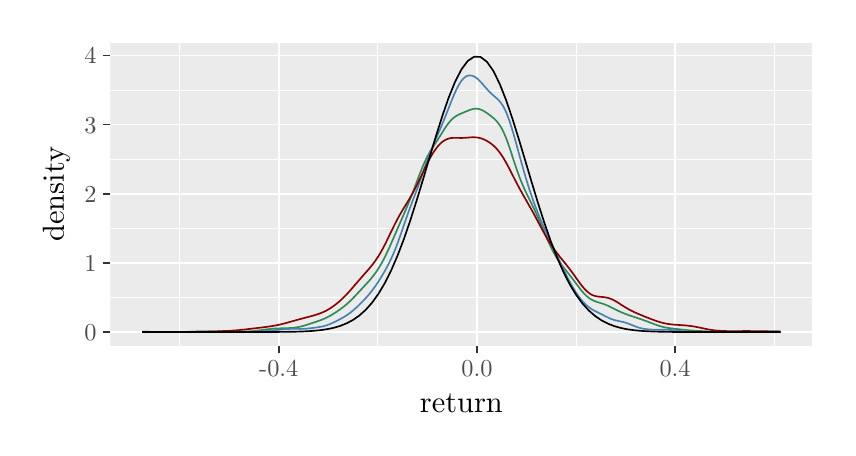
\begin{tikzpicture}[x=1pt,y=1pt]
\definecolor{fillColor}{RGB}{255,255,255}
\path[use as bounding box,fill=fillColor,fill opacity=0.00] (0,0) rectangle (289.08,144.54);
\begin{scope}
\path[clip] (  0.00,  0.00) rectangle (289.08,144.54);
\definecolor{drawColor}{RGB}{255,255,255}
\definecolor{fillColor}{RGB}{255,255,255}

\path[draw=drawColor,line width= 0.6pt,line join=round,line cap=round,fill=fillColor] (  0.00,  0.00) rectangle (289.08,144.54);
\end{scope}
\begin{scope}
\path[clip] ( 29.87, 29.59) rectangle (283.58,139.04);
\definecolor{fillColor}{gray}{0.92}

\path[fill=fillColor] ( 29.87, 29.59) rectangle (283.58,139.04);
\definecolor{drawColor}{RGB}{255,255,255}

\path[draw=drawColor,line width= 0.3pt,line join=round] ( 29.87, 47.05) --
	(283.58, 47.05);

\path[draw=drawColor,line width= 0.3pt,line join=round] ( 29.87, 72.03) --
	(283.58, 72.03);

\path[draw=drawColor,line width= 0.3pt,line join=round] ( 29.87, 97.01) --
	(283.58, 97.01);

\path[draw=drawColor,line width= 0.3pt,line join=round] ( 29.87,121.99) --
	(283.58,121.99);

\path[draw=drawColor,line width= 0.3pt,line join=round] ( 54.93, 29.59) --
	( 54.93,139.04);

\path[draw=drawColor,line width= 0.3pt,line join=round] (126.54, 29.59) --
	(126.54,139.04);

\path[draw=drawColor,line width= 0.3pt,line join=round] (198.14, 29.59) --
	(198.14,139.04);

\path[draw=drawColor,line width= 0.3pt,line join=round] (269.75, 29.59) --
	(269.75,139.04);

\path[draw=drawColor,line width= 0.6pt,line join=round] ( 29.87, 34.56) --
	(283.58, 34.56);

\path[draw=drawColor,line width= 0.6pt,line join=round] ( 29.87, 59.54) --
	(283.58, 59.54);

\path[draw=drawColor,line width= 0.6pt,line join=round] ( 29.87, 84.52) --
	(283.58, 84.52);

\path[draw=drawColor,line width= 0.6pt,line join=round] ( 29.87,109.50) --
	(283.58,109.50);

\path[draw=drawColor,line width= 0.6pt,line join=round] ( 29.87,134.48) --
	(283.58,134.48);

\path[draw=drawColor,line width= 0.6pt,line join=round] ( 90.73, 29.59) --
	( 90.73,139.04);

\path[draw=drawColor,line width= 0.6pt,line join=round] (162.34, 29.59) --
	(162.34,139.04);

\path[draw=drawColor,line width= 0.6pt,line join=round] (233.94, 29.59) --
	(233.94,139.04);
\definecolor{drawColor}{RGB}{46,139,87}

\path[draw=drawColor,line width= 0.6pt,line join=round] ( 41.40, 34.56) --
	( 41.85, 34.56) --
	( 42.30, 34.56) --
	( 42.76, 34.56) --
	( 43.21, 34.56) --
	( 43.66, 34.56) --
	( 44.11, 34.56) --
	( 44.56, 34.56) --
	( 45.01, 34.56) --
	( 45.46, 34.56) --
	( 45.91, 34.56) --
	( 46.37, 34.56) --
	( 46.82, 34.56) --
	( 47.27, 34.56) --
	( 47.72, 34.56) --
	( 48.17, 34.56) --
	( 48.62, 34.56) --
	( 49.07, 34.56) --
	( 49.53, 34.56) --
	( 49.98, 34.56) --
	( 50.43, 34.56) --
	( 50.88, 34.56) --
	( 51.33, 34.56) --
	( 51.78, 34.56) --
	( 52.23, 34.56) --
	( 52.69, 34.57) --
	( 53.14, 34.57) --
	( 53.59, 34.57) --
	( 54.04, 34.57) --
	( 54.49, 34.58) --
	( 54.94, 34.58) --
	( 55.39, 34.59) --
	( 55.84, 34.59) --
	( 56.30, 34.60) --
	( 56.75, 34.61) --
	( 57.20, 34.62) --
	( 57.65, 34.63) --
	( 58.10, 34.64) --
	( 58.55, 34.65) --
	( 59.00, 34.67) --
	( 59.46, 34.68) --
	( 59.91, 34.70) --
	( 60.36, 34.71) --
	( 60.81, 34.72) --
	( 61.26, 34.73) --
	( 61.71, 34.74) --
	( 62.16, 34.75) --
	( 62.62, 34.75) --
	( 63.07, 34.75) --
	( 63.52, 34.76) --
	( 63.97, 34.75) --
	( 64.42, 34.75) --
	( 64.87, 34.75) --
	( 65.32, 34.74) --
	( 65.77, 34.74) --
	( 66.23, 34.73) --
	( 66.68, 34.73) --
	( 67.13, 34.73) --
	( 67.58, 34.73) --
	( 68.03, 34.73) --
	( 68.48, 34.73) --
	( 68.93, 34.73) --
	( 69.39, 34.74) --
	( 69.84, 34.74) --
	( 70.29, 34.75) --
	( 70.74, 34.76) --
	( 71.19, 34.76) --
	( 71.64, 34.77) --
	( 72.09, 34.77) --
	( 72.55, 34.77) --
	( 73.00, 34.77) --
	( 73.45, 34.77) --
	( 73.90, 34.76) --
	( 74.35, 34.76) --
	( 74.80, 34.75) --
	( 75.25, 34.74) --
	( 75.70, 34.73) --
	( 76.16, 34.73) --
	( 76.61, 34.72) --
	( 77.06, 34.72) --
	( 77.51, 34.72) --
	( 77.96, 34.72) --
	( 78.41, 34.73) --
	( 78.86, 34.74) --
	( 79.32, 34.76) --
	( 79.77, 34.79) --
	( 80.22, 34.81) --
	( 80.67, 34.85) --
	( 81.12, 34.88) --
	( 81.57, 34.92) --
	( 82.02, 34.97) --
	( 82.48, 35.02) --
	( 82.93, 35.07) --
	( 83.38, 35.13) --
	( 83.83, 35.19) --
	( 84.28, 35.25) --
	( 84.73, 35.31) --
	( 85.18, 35.38) --
	( 85.63, 35.44) --
	( 86.09, 35.50) --
	( 86.54, 35.56) --
	( 86.99, 35.61) --
	( 87.44, 35.66) --
	( 87.89, 35.70) --
	( 88.34, 35.74) --
	( 88.79, 35.78) --
	( 89.25, 35.81) --
	( 89.70, 35.83) --
	( 90.15, 35.85) --
	( 90.60, 35.87) --
	( 91.05, 35.88) --
	( 91.50, 35.90) --
	( 91.95, 35.91) --
	( 92.41, 35.92) --
	( 92.86, 35.93) --
	( 93.31, 35.94) --
	( 93.76, 35.96) --
	( 94.21, 35.98) --
	( 94.66, 36.00) --
	( 95.11, 36.03) --
	( 95.56, 36.06) --
	( 96.02, 36.10) --
	( 96.47, 36.16) --
	( 96.92, 36.22) --
	( 97.37, 36.29) --
	( 97.82, 36.37) --
	( 98.27, 36.46) --
	( 98.72, 36.56) --
	( 99.18, 36.67) --
	( 99.63, 36.79) --
	(100.08, 36.92) --
	(100.53, 37.06) --
	(100.98, 37.20) --
	(101.43, 37.35) --
	(101.88, 37.50) --
	(102.34, 37.65) --
	(102.79, 37.80) --
	(103.24, 37.94) --
	(103.69, 38.09) --
	(104.14, 38.24) --
	(104.59, 38.40) --
	(105.04, 38.55) --
	(105.49, 38.71) --
	(105.95, 38.88) --
	(106.40, 39.05) --
	(106.85, 39.23) --
	(107.30, 39.43) --
	(107.75, 39.64) --
	(108.20, 39.86) --
	(108.65, 40.09) --
	(109.11, 40.33) --
	(109.56, 40.59) --
	(110.01, 40.85) --
	(110.46, 41.13) --
	(110.91, 41.41) --
	(111.36, 41.70) --
	(111.81, 42.00) --
	(112.27, 42.31) --
	(112.72, 42.62) --
	(113.17, 42.95) --
	(113.62, 43.29) --
	(114.07, 43.63) --
	(114.52, 43.99) --
	(114.97, 44.37) --
	(115.42, 44.76) --
	(115.88, 45.16) --
	(116.33, 45.58) --
	(116.78, 46.02) --
	(117.23, 46.46) --
	(117.68, 46.92) --
	(118.13, 47.39) --
	(118.58, 47.87) --
	(119.04, 48.35) --
	(119.49, 48.84) --
	(119.94, 49.33) --
	(120.39, 49.81) --
	(120.84, 50.30) --
	(121.29, 50.78) --
	(121.74, 51.27) --
	(122.20, 51.76) --
	(122.65, 52.25) --
	(123.10, 52.75) --
	(123.55, 53.26) --
	(124.00, 53.78) --
	(124.45, 54.33) --
	(124.90, 54.90) --
	(125.35, 55.49) --
	(125.81, 56.11) --
	(126.26, 56.77) --
	(126.71, 57.46) --
	(127.16, 58.18) --
	(127.61, 58.94) --
	(128.06, 59.74) --
	(128.51, 60.58) --
	(128.97, 61.46) --
	(129.42, 62.37) --
	(129.87, 63.31) --
	(130.32, 64.28) --
	(130.77, 65.28) --
	(131.22, 66.29) --
	(131.67, 67.32) --
	(132.13, 68.36) --
	(132.58, 69.41) --
	(133.03, 70.45) --
	(133.48, 71.50) --
	(133.93, 72.54) --
	(134.38, 73.58) --
	(134.83, 74.62) --
	(135.28, 75.65) --
	(135.74, 76.69) --
	(136.19, 77.73) --
	(136.64, 78.78) --
	(137.09, 79.85) --
	(137.54, 80.94) --
	(137.99, 82.05) --
	(138.44, 83.18) --
	(138.90, 84.33) --
	(139.35, 85.51) --
	(139.80, 86.70) --
	(140.25, 87.91) --
	(140.70, 89.12) --
	(141.15, 90.32) --
	(141.60, 91.50) --
	(142.06, 92.65) --
	(142.51, 93.77) --
	(142.96, 94.85) --
	(143.41, 95.87) --
	(143.86, 96.83) --
	(144.31, 97.74) --
	(144.76, 98.59) --
	(145.21, 99.39) --
	(145.67,100.15) --
	(146.12,100.88) --
	(146.57,101.59) --
	(147.02,102.28) --
	(147.47,102.97) --
	(147.92,103.67) --
	(148.37,104.37) --
	(148.83,105.08) --
	(149.28,105.80) --
	(149.73,106.53) --
	(150.18,107.25) --
	(150.63,107.96) --
	(151.08,108.64) --
	(151.53,109.30) --
	(151.99,109.92) --
	(152.44,110.49) --
	(152.89,111.01) --
	(153.34,111.46) --
	(153.79,111.87) --
	(154.24,112.22) --
	(154.69,112.53) --
	(155.14,112.80) --
	(155.60,113.04) --
	(156.05,113.26) --
	(156.50,113.46) --
	(156.95,113.65) --
	(157.40,113.84) --
	(157.85,114.03) --
	(158.30,114.22) --
	(158.76,114.41) --
	(159.21,114.59) --
	(159.66,114.77) --
	(160.11,114.93) --
	(160.56,115.07) --
	(161.01,115.18) --
	(161.46,115.25) --
	(161.92,115.28) --
	(162.37,115.26) --
	(162.82,115.20) --
	(163.27,115.09) --
	(163.72,114.93) --
	(164.17,114.74) --
	(164.62,114.51) --
	(165.07,114.25) --
	(165.53,113.96) --
	(165.98,113.65) --
	(166.43,113.34) --
	(166.88,113.01) --
	(167.33,112.67) --
	(167.78,112.32) --
	(168.23,111.94) --
	(168.69,111.54) --
	(169.14,111.10) --
	(169.59,110.61) --
	(170.04,110.05) --
	(170.49,109.43) --
	(170.94,108.72) --
	(171.39,107.92) --
	(171.85,107.02) --
	(172.30,106.03) --
	(172.75,104.96) --
	(173.20,103.79) --
	(173.65,102.54) --
	(174.10,101.23) --
	(174.55, 99.88) --
	(175.00, 98.51) --
	(175.46, 97.12) --
	(175.91, 95.74) --
	(176.36, 94.38) --
	(176.81, 93.06) --
	(177.26, 91.78) --
	(177.71, 90.56) --
	(178.16, 89.39) --
	(178.62, 88.28) --
	(179.07, 87.22) --
	(179.52, 86.21) --
	(179.97, 85.23) --
	(180.42, 84.29) --
	(180.87, 83.36) --
	(181.32, 82.45) --
	(181.78, 81.54) --
	(182.23, 80.62) --
	(182.68, 79.68) --
	(183.13, 78.73) --
	(183.58, 77.76) --
	(184.03, 76.76) --
	(184.48, 75.74) --
	(184.93, 74.70) --
	(185.39, 73.65) --
	(185.84, 72.58) --
	(186.29, 71.51) --
	(186.74, 70.45) --
	(187.19, 69.39) --
	(187.64, 68.35) --
	(188.09, 67.34) --
	(188.55, 66.35) --
	(189.00, 65.39) --
	(189.45, 64.48) --
	(189.90, 63.61) --
	(190.35, 62.78) --
	(190.80, 62.00) --
	(191.25, 61.26) --
	(191.71, 60.56) --
	(192.16, 59.89) --
	(192.61, 59.26) --
	(193.06, 58.65) --
	(193.51, 58.07) --
	(193.96, 57.50) --
	(194.41, 56.94) --
	(194.86, 56.38) --
	(195.32, 55.81) --
	(195.77, 55.25) --
	(196.22, 54.67) --
	(196.67, 54.08) --
	(197.12, 53.49) --
	(197.57, 52.89) --
	(198.02, 52.28) --
	(198.48, 51.67) --
	(198.93, 51.07) --
	(199.38, 50.47) --
	(199.83, 49.90) --
	(200.28, 49.34) --
	(200.73, 48.82) --
	(201.18, 48.32) --
	(201.64, 47.86) --
	(202.09, 47.45) --
	(202.54, 47.07) --
	(202.99, 46.74) --
	(203.44, 46.45) --
	(203.89, 46.19) --
	(204.34, 45.96) --
	(204.79, 45.77) --
	(205.25, 45.60) --
	(205.70, 45.44) --
	(206.15, 45.30) --
	(206.60, 45.16) --
	(207.05, 45.02) --
	(207.50, 44.88) --
	(207.95, 44.73) --
	(208.41, 44.57) --
	(208.86, 44.39) --
	(209.31, 44.21) --
	(209.76, 44.01) --
	(210.21, 43.80) --
	(210.66, 43.58) --
	(211.11, 43.35) --
	(211.57, 43.13) --
	(212.02, 42.90) --
	(212.47, 42.67) --
	(212.92, 42.45) --
	(213.37, 42.23) --
	(213.82, 42.02) --
	(214.27, 41.82) --
	(214.72, 41.62) --
	(215.18, 41.43) --
	(215.63, 41.25) --
	(216.08, 41.08) --
	(216.53, 40.91) --
	(216.98, 40.74) --
	(217.43, 40.58) --
	(217.88, 40.43) --
	(218.34, 40.27) --
	(218.79, 40.12) --
	(219.24, 39.97) --
	(219.69, 39.82) --
	(220.14, 39.68) --
	(220.59, 39.53) --
	(221.04, 39.38) --
	(221.50, 39.22) --
	(221.95, 39.07) --
	(222.40, 38.91) --
	(222.85, 38.75) --
	(223.30, 38.58) --
	(223.75, 38.41) --
	(224.20, 38.24) --
	(224.65, 38.07) --
	(225.11, 37.89) --
	(225.56, 37.72) --
	(226.01, 37.55) --
	(226.46, 37.38) --
	(226.91, 37.21) --
	(227.36, 37.05) --
	(227.81, 36.90) --
	(228.27, 36.76) --
	(228.72, 36.62) --
	(229.17, 36.50) --
	(229.62, 36.39) --
	(230.07, 36.28) --
	(230.52, 36.19) --
	(230.97, 36.11) --
	(231.43, 36.04) --
	(231.88, 35.97) --
	(232.33, 35.91) --
	(232.78, 35.85) --
	(233.23, 35.80) --
	(233.68, 35.75) --
	(234.13, 35.70) --
	(234.58, 35.65) --
	(235.04, 35.60) --
	(235.49, 35.55) --
	(235.94, 35.50) --
	(236.39, 35.45) --
	(236.84, 35.41) --
	(237.29, 35.36) --
	(237.74, 35.31) --
	(238.20, 35.27) --
	(238.65, 35.23) --
	(239.10, 35.19) --
	(239.55, 35.15) --
	(240.00, 35.12) --
	(240.45, 35.09) --
	(240.90, 35.06) --
	(241.35, 35.04) --
	(241.81, 35.01) --
	(242.26, 34.99) --
	(242.71, 34.96) --
	(243.16, 34.94) --
	(243.61, 34.91) --
	(244.06, 34.88) --
	(244.51, 34.85) --
	(244.97, 34.83) --
	(245.42, 34.80) --
	(245.87, 34.77) --
	(246.32, 34.74) --
	(246.77, 34.72) --
	(247.22, 34.69) --
	(247.67, 34.67) --
	(248.13, 34.65) --
	(248.58, 34.64) --
	(249.03, 34.62) --
	(249.48, 34.61) --
	(249.93, 34.60) --
	(250.38, 34.59) --
	(250.83, 34.58) --
	(251.28, 34.58) --
	(251.74, 34.57) --
	(252.19, 34.57) --
	(252.64, 34.57) --
	(253.09, 34.57) --
	(253.54, 34.56) --
	(253.99, 34.56) --
	(254.44, 34.56) --
	(254.90, 34.56) --
	(255.35, 34.56) --
	(255.80, 34.56) --
	(256.25, 34.56) --
	(256.70, 34.56) --
	(257.15, 34.56) --
	(257.60, 34.57) --
	(258.06, 34.57) --
	(258.51, 34.57) --
	(258.96, 34.57) --
	(259.41, 34.58) --
	(259.86, 34.58) --
	(260.31, 34.58) --
	(260.76, 34.59) --
	(261.21, 34.60) --
	(261.67, 34.60) --
	(262.12, 34.61) --
	(262.57, 34.62) --
	(263.02, 34.63) --
	(263.47, 34.65) --
	(263.92, 34.66) --
	(264.37, 34.67) --
	(264.83, 34.69) --
	(265.28, 34.70) --
	(265.73, 34.71) --
	(266.18, 34.73) --
	(266.63, 34.74) --
	(267.08, 34.76) --
	(267.53, 34.77) --
	(267.99, 34.78) --
	(268.44, 34.79) --
	(268.89, 34.80) --
	(269.34, 34.80) --
	(269.79, 34.81) --
	(270.24, 34.81) --
	(270.69, 34.81) --
	(271.14, 34.80) --
	(271.60, 34.80) --
	(272.05, 34.79);
\definecolor{drawColor}{RGB}{70,130,180}

\path[draw=drawColor,line width= 0.6pt,line join=round] ( 41.40, 34.56) --
	( 41.85, 34.56) --
	( 42.30, 34.56) --
	( 42.76, 34.56) --
	( 43.21, 34.56) --
	( 43.66, 34.56) --
	( 44.11, 34.56) --
	( 44.56, 34.56) --
	( 45.01, 34.56) --
	( 45.46, 34.56) --
	( 45.91, 34.56) --
	( 46.37, 34.56) --
	( 46.82, 34.56) --
	( 47.27, 34.56) --
	( 47.72, 34.56) --
	( 48.17, 34.56) --
	( 48.62, 34.56) --
	( 49.07, 34.56) --
	( 49.53, 34.56) --
	( 49.98, 34.56) --
	( 50.43, 34.56) --
	( 50.88, 34.56) --
	( 51.33, 34.56) --
	( 51.78, 34.56) --
	( 52.23, 34.56) --
	( 52.69, 34.56) --
	( 53.14, 34.56) --
	( 53.59, 34.56) --
	( 54.04, 34.57) --
	( 54.49, 34.57) --
	( 54.94, 34.57) --
	( 55.39, 34.57) --
	( 55.84, 34.58) --
	( 56.30, 34.58) --
	( 56.75, 34.59) --
	( 57.20, 34.59) --
	( 57.65, 34.60) --
	( 58.10, 34.61) --
	( 58.55, 34.62) --
	( 59.00, 34.63) --
	( 59.46, 34.64) --
	( 59.91, 34.65) --
	( 60.36, 34.66) --
	( 60.81, 34.66) --
	( 61.26, 34.67) --
	( 61.71, 34.67) --
	( 62.16, 34.67) --
	( 62.62, 34.67) --
	( 63.07, 34.67) --
	( 63.52, 34.67) --
	( 63.97, 34.66) --
	( 64.42, 34.65) --
	( 64.87, 34.64) --
	( 65.32, 34.63) --
	( 65.77, 34.62) --
	( 66.23, 34.61) --
	( 66.68, 34.60) --
	( 67.13, 34.60) --
	( 67.58, 34.59) --
	( 68.03, 34.58) --
	( 68.48, 34.58) --
	( 68.93, 34.57) --
	( 69.39, 34.57) --
	( 69.84, 34.57) --
	( 70.29, 34.57) --
	( 70.74, 34.57) --
	( 71.19, 34.56) --
	( 71.64, 34.56) --
	( 72.09, 34.56) --
	( 72.55, 34.56) --
	( 73.00, 34.56) --
	( 73.45, 34.56) --
	( 73.90, 34.56) --
	( 74.35, 34.56) --
	( 74.80, 34.56) --
	( 75.25, 34.56) --
	( 75.70, 34.56) --
	( 76.16, 34.56) --
	( 76.61, 34.56) --
	( 77.06, 34.56) --
	( 77.51, 34.56) --
	( 77.96, 34.57) --
	( 78.41, 34.57) --
	( 78.86, 34.57) --
	( 79.32, 34.57) --
	( 79.77, 34.58) --
	( 80.22, 34.58) --
	( 80.67, 34.59) --
	( 81.12, 34.60) --
	( 81.57, 34.61) --
	( 82.02, 34.63) --
	( 82.48, 34.65) --
	( 82.93, 34.67) --
	( 83.38, 34.69) --
	( 83.83, 34.72) --
	( 84.28, 34.75) --
	( 84.73, 34.79) --
	( 85.18, 34.83) --
	( 85.63, 34.87) --
	( 86.09, 34.91) --
	( 86.54, 34.96) --
	( 86.99, 35.00) --
	( 87.44, 35.05) --
	( 87.89, 35.09) --
	( 88.34, 35.14) --
	( 88.79, 35.18) --
	( 89.25, 35.23) --
	( 89.70, 35.27) --
	( 90.15, 35.31) --
	( 90.60, 35.36) --
	( 91.05, 35.40) --
	( 91.50, 35.44) --
	( 91.95, 35.48) --
	( 92.41, 35.52) --
	( 92.86, 35.56) --
	( 93.31, 35.60) --
	( 93.76, 35.63) --
	( 94.21, 35.66) --
	( 94.66, 35.68) --
	( 95.11, 35.70) --
	( 95.56, 35.71) --
	( 96.02, 35.71) --
	( 96.47, 35.71) --
	( 96.92, 35.70) --
	( 97.37, 35.69) --
	( 97.82, 35.69) --
	( 98.27, 35.68) --
	( 98.72, 35.69) --
	( 99.18, 35.69) --
	( 99.63, 35.71) --
	(100.08, 35.73) --
	(100.53, 35.76) --
	(100.98, 35.80) --
	(101.43, 35.85) --
	(101.88, 35.90) --
	(102.34, 35.95) --
	(102.79, 36.01) --
	(103.24, 36.07) --
	(103.69, 36.13) --
	(104.14, 36.19) --
	(104.59, 36.25) --
	(105.04, 36.32) --
	(105.49, 36.39) --
	(105.95, 36.47) --
	(106.40, 36.56) --
	(106.85, 36.66) --
	(107.30, 36.78) --
	(107.75, 36.91) --
	(108.20, 37.06) --
	(108.65, 37.22) --
	(109.11, 37.39) --
	(109.56, 37.58) --
	(110.01, 37.78) --
	(110.46, 37.99) --
	(110.91, 38.20) --
	(111.36, 38.42) --
	(111.81, 38.65) --
	(112.27, 38.88) --
	(112.72, 39.11) --
	(113.17, 39.36) --
	(113.62, 39.61) --
	(114.07, 39.86) --
	(114.52, 40.13) --
	(114.97, 40.42) --
	(115.42, 40.71) --
	(115.88, 41.03) --
	(116.33, 41.36) --
	(116.78, 41.70) --
	(117.23, 42.07) --
	(117.68, 42.45) --
	(118.13, 42.84) --
	(118.58, 43.25) --
	(119.04, 43.66) --
	(119.49, 44.09) --
	(119.94, 44.53) --
	(120.39, 44.98) --
	(120.84, 45.43) --
	(121.29, 45.89) --
	(121.74, 46.37) --
	(122.20, 46.85) --
	(122.65, 47.36) --
	(123.10, 47.87) --
	(123.55, 48.41) --
	(124.00, 48.97) --
	(124.45, 49.54) --
	(124.90, 50.14) --
	(125.35, 50.77) --
	(125.81, 51.41) --
	(126.26, 52.08) --
	(126.71, 52.76) --
	(127.16, 53.47) --
	(127.61, 54.19) --
	(128.06, 54.93) --
	(128.51, 55.70) --
	(128.97, 56.48) --
	(129.42, 57.28) --
	(129.87, 58.12) --
	(130.32, 58.98) --
	(130.77, 59.87) --
	(131.22, 60.80) --
	(131.67, 61.78) --
	(132.13, 62.80) --
	(132.58, 63.87) --
	(133.03, 64.99) --
	(133.48, 66.16) --
	(133.93, 67.38) --
	(134.38, 68.65) --
	(134.83, 69.94) --
	(135.28, 71.25) --
	(135.74, 72.58) --
	(136.19, 73.90) --
	(136.64, 75.21) --
	(137.09, 76.49) --
	(137.54, 77.76) --
	(137.99, 79.00) --
	(138.44, 80.21) --
	(138.90, 81.41) --
	(139.35, 82.59) --
	(139.80, 83.77) --
	(140.25, 84.96) --
	(140.70, 86.16) --
	(141.15, 87.39) --
	(141.60, 88.63) --
	(142.06, 89.90) --
	(142.51, 91.18) --
	(142.96, 92.48) --
	(143.41, 93.78) --
	(143.86, 95.07) --
	(144.31, 96.34) --
	(144.76, 97.58) --
	(145.21, 98.78) --
	(145.67, 99.95) --
	(146.12,101.09) --
	(146.57,102.18) --
	(147.02,103.25) --
	(147.47,104.30) --
	(147.92,105.33) --
	(148.37,106.36) --
	(148.83,107.39) --
	(149.28,108.45) --
	(149.73,109.52) --
	(150.18,110.61) --
	(150.63,111.72) --
	(151.08,112.85) --
	(151.53,114.00) --
	(151.99,115.15) --
	(152.44,116.31) --
	(152.89,117.45) --
	(153.34,118.57) --
	(153.79,119.66) --
	(154.24,120.70) --
	(154.69,121.69) --
	(155.14,122.63) --
	(155.60,123.49) --
	(156.05,124.27) --
	(156.50,124.97) --
	(156.95,125.58) --
	(157.40,126.09) --
	(157.85,126.51) --
	(158.30,126.83) --
	(158.76,127.07) --
	(159.21,127.22) --
	(159.66,127.29) --
	(160.11,127.28) --
	(160.56,127.19) --
	(161.01,127.04) --
	(161.46,126.82) --
	(161.92,126.54) --
	(162.37,126.20) --
	(162.82,125.82) --
	(163.27,125.38) --
	(163.72,124.92) --
	(164.17,124.42) --
	(164.62,123.90) --
	(165.07,123.37) --
	(165.53,122.84) --
	(165.98,122.32) --
	(166.43,121.82) --
	(166.88,121.35) --
	(167.33,120.90) --
	(167.78,120.48) --
	(168.23,120.08) --
	(168.69,119.69) --
	(169.14,119.31) --
	(169.59,118.91) --
	(170.04,118.49) --
	(170.49,118.01) --
	(170.94,117.46) --
	(171.39,116.83) --
	(171.85,116.09) --
	(172.30,115.25) --
	(172.75,114.31) --
	(173.20,113.24) --
	(173.65,112.07) --
	(174.10,110.80) --
	(174.55,109.43) --
	(175.00,107.99) --
	(175.46,106.46) --
	(175.91,104.88) --
	(176.36,103.27) --
	(176.81,101.63) --
	(177.26, 99.98) --
	(177.71, 98.33) --
	(178.16, 96.69) --
	(178.62, 95.07) --
	(179.07, 93.47) --
	(179.52, 91.90) --
	(179.97, 90.37) --
	(180.42, 88.89) --
	(180.87, 87.44) --
	(181.32, 86.03) --
	(181.78, 84.67) --
	(182.23, 83.34) --
	(182.68, 82.06) --
	(183.13, 80.81) --
	(183.58, 79.59) --
	(184.03, 78.42) --
	(184.48, 77.27) --
	(184.93, 76.16) --
	(185.39, 75.08) --
	(185.84, 74.02) --
	(186.29, 72.98) --
	(186.74, 71.96) --
	(187.19, 70.96) --
	(187.64, 69.97) --
	(188.09, 68.99) --
	(188.55, 68.02) --
	(189.00, 67.06) --
	(189.45, 66.10) --
	(189.90, 65.14) --
	(190.35, 64.18) --
	(190.80, 63.22) --
	(191.25, 62.26) --
	(191.71, 61.30) --
	(192.16, 60.33) --
	(192.61, 59.37) --
	(193.06, 58.41) --
	(193.51, 57.46) --
	(193.96, 56.52) --
	(194.41, 55.59) --
	(194.86, 54.68) --
	(195.32, 53.80) --
	(195.77, 52.93) --
	(196.22, 52.10) --
	(196.67, 51.29) --
	(197.12, 50.51) --
	(197.57, 49.76) --
	(198.02, 49.04) --
	(198.48, 48.36) --
	(198.93, 47.71) --
	(199.38, 47.09) --
	(199.83, 46.51) --
	(200.28, 45.95) --
	(200.73, 45.44) --
	(201.18, 44.95) --
	(201.64, 44.50) --
	(202.09, 44.09) --
	(202.54, 43.71) --
	(202.99, 43.37) --
	(203.44, 43.06) --
	(203.89, 42.77) --
	(204.34, 42.51) --
	(204.79, 42.26) --
	(205.25, 42.02) --
	(205.70, 41.80) --
	(206.15, 41.58) --
	(206.60, 41.36) --
	(207.05, 41.13) --
	(207.50, 40.90) --
	(207.95, 40.67) --
	(208.41, 40.44) --
	(208.86, 40.20) --
	(209.31, 39.98) --
	(209.76, 39.76) --
	(210.21, 39.55) --
	(210.66, 39.36) --
	(211.11, 39.19) --
	(211.57, 39.03) --
	(212.02, 38.90) --
	(212.47, 38.78) --
	(212.92, 38.67) --
	(213.37, 38.57) --
	(213.82, 38.48) --
	(214.27, 38.39) --
	(214.72, 38.29) --
	(215.18, 38.18) --
	(215.63, 38.06) --
	(216.08, 37.93) --
	(216.53, 37.78) --
	(216.98, 37.62) --
	(217.43, 37.45) --
	(217.88, 37.27) --
	(218.34, 37.08) --
	(218.79, 36.90) --
	(219.24, 36.72) --
	(219.69, 36.54) --
	(220.14, 36.38) --
	(220.59, 36.22) --
	(221.04, 36.09) --
	(221.50, 35.97) --
	(221.95, 35.86) --
	(222.40, 35.77) --
	(222.85, 35.69) --
	(223.30, 35.63) --
	(223.75, 35.57) --
	(224.20, 35.53) --
	(224.65, 35.49) --
	(225.11, 35.46) --
	(225.56, 35.44) --
	(226.01, 35.42) --
	(226.46, 35.40) --
	(226.91, 35.39) --
	(227.36, 35.38) --
	(227.81, 35.38) --
	(228.27, 35.37) --
	(228.72, 35.37) --
	(229.17, 35.37) --
	(229.62, 35.37) --
	(230.07, 35.36) --
	(230.52, 35.36) --
	(230.97, 35.35) --
	(231.43, 35.34) --
	(231.88, 35.32) --
	(232.33, 35.29) --
	(232.78, 35.26) --
	(233.23, 35.23) --
	(233.68, 35.19) --
	(234.13, 35.14) --
	(234.58, 35.09) --
	(235.04, 35.04) --
	(235.49, 34.99) --
	(235.94, 34.94) --
	(236.39, 34.89) --
	(236.84, 34.84) --
	(237.29, 34.79) --
	(237.74, 34.75) --
	(238.20, 34.72) --
	(238.65, 34.69) --
	(239.10, 34.66) --
	(239.55, 34.64) --
	(240.00, 34.62) --
	(240.45, 34.61) --
	(240.90, 34.59) --
	(241.35, 34.59) --
	(241.81, 34.58) --
	(242.26, 34.57) --
	(242.71, 34.57) --
	(243.16, 34.57) --
	(243.61, 34.57) --
	(244.06, 34.56) --
	(244.51, 34.56) --
	(244.97, 34.56) --
	(245.42, 34.56) --
	(245.87, 34.56) --
	(246.32, 34.56) --
	(246.77, 34.56) --
	(247.22, 34.56) --
	(247.67, 34.56) --
	(248.13, 34.56) --
	(248.58, 34.56) --
	(249.03, 34.56) --
	(249.48, 34.56) --
	(249.93, 34.56) --
	(250.38, 34.57) --
	(250.83, 34.57) --
	(251.28, 34.57) --
	(251.74, 34.57) --
	(252.19, 34.58) --
	(252.64, 34.58) --
	(253.09, 34.58) --
	(253.54, 34.59) --
	(253.99, 34.60) --
	(254.44, 34.61) --
	(254.90, 34.62) --
	(255.35, 34.63) --
	(255.80, 34.63) --
	(256.25, 34.64) --
	(256.70, 34.65) --
	(257.15, 34.66) --
	(257.60, 34.67) --
	(258.06, 34.67) --
	(258.51, 34.67) --
	(258.96, 34.67) --
	(259.41, 34.67) --
	(259.86, 34.67) --
	(260.31, 34.66) --
	(260.76, 34.65) --
	(261.21, 34.65) --
	(261.67, 34.64) --
	(262.12, 34.63) --
	(262.57, 34.62) --
	(263.02, 34.61) --
	(263.47, 34.60) --
	(263.92, 34.59) --
	(264.37, 34.59) --
	(264.83, 34.58) --
	(265.28, 34.58) --
	(265.73, 34.57) --
	(266.18, 34.57) --
	(266.63, 34.57) --
	(267.08, 34.57) --
	(267.53, 34.56) --
	(267.99, 34.56) --
	(268.44, 34.56) --
	(268.89, 34.56) --
	(269.34, 34.56) --
	(269.79, 34.56) --
	(270.24, 34.56) --
	(270.69, 34.56) --
	(271.14, 34.56) --
	(271.60, 34.56) --
	(272.05, 34.56);
\definecolor{drawColor}{RGB}{139,0,0}

\path[draw=drawColor,line width= 0.6pt,line join=round] ( 41.40, 34.65) --
	( 41.85, 34.65) --
	( 42.30, 34.65) --
	( 42.76, 34.65) --
	( 43.21, 34.64) --
	( 43.66, 34.64) --
	( 44.11, 34.63) --
	( 44.56, 34.63) --
	( 45.01, 34.62) --
	( 45.46, 34.62) --
	( 45.91, 34.61) --
	( 46.37, 34.60) --
	( 46.82, 34.60) --
	( 47.27, 34.59) --
	( 47.72, 34.59) --
	( 48.17, 34.58) --
	( 48.62, 34.58) --
	( 49.07, 34.58) --
	( 49.53, 34.57) --
	( 49.98, 34.57) --
	( 50.43, 34.57) --
	( 50.88, 34.57) --
	( 51.33, 34.57) --
	( 51.78, 34.57) --
	( 52.23, 34.57) --
	( 52.69, 34.57) --
	( 53.14, 34.57) --
	( 53.59, 34.57) --
	( 54.04, 34.57) --
	( 54.49, 34.57) --
	( 54.94, 34.57) --
	( 55.39, 34.57) --
	( 55.84, 34.57) --
	( 56.30, 34.58) --
	( 56.75, 34.58) --
	( 57.20, 34.58) --
	( 57.65, 34.59) --
	( 58.10, 34.59) --
	( 58.55, 34.60) --
	( 59.00, 34.61) --
	( 59.46, 34.61) --
	( 59.91, 34.62) --
	( 60.36, 34.63) --
	( 60.81, 34.63) --
	( 61.26, 34.64) --
	( 61.71, 34.65) --
	( 62.16, 34.66) --
	( 62.62, 34.67) --
	( 63.07, 34.67) --
	( 63.52, 34.68) --
	( 63.97, 34.69) --
	( 64.42, 34.70) --
	( 64.87, 34.71) --
	( 65.32, 34.72) --
	( 65.77, 34.73) --
	( 66.23, 34.74) --
	( 66.68, 34.75) --
	( 67.13, 34.77) --
	( 67.58, 34.78) --
	( 68.03, 34.79) --
	( 68.48, 34.81) --
	( 68.93, 34.83) --
	( 69.39, 34.85) --
	( 69.84, 34.87) --
	( 70.29, 34.89) --
	( 70.74, 34.91) --
	( 71.19, 34.93) --
	( 71.64, 34.95) --
	( 72.09, 34.97) --
	( 72.55, 34.99) --
	( 73.00, 35.02) --
	( 73.45, 35.04) --
	( 73.90, 35.07) --
	( 74.35, 35.10) --
	( 74.80, 35.13) --
	( 75.25, 35.17) --
	( 75.70, 35.21) --
	( 76.16, 35.25) --
	( 76.61, 35.29) --
	( 77.06, 35.33) --
	( 77.51, 35.38) --
	( 77.96, 35.43) --
	( 78.41, 35.48) --
	( 78.86, 35.53) --
	( 79.32, 35.58) --
	( 79.77, 35.63) --
	( 80.22, 35.68) --
	( 80.67, 35.74) --
	( 81.12, 35.79) --
	( 81.57, 35.85) --
	( 82.02, 35.90) --
	( 82.48, 35.95) --
	( 82.93, 36.01) --
	( 83.38, 36.06) --
	( 83.83, 36.12) --
	( 84.28, 36.17) --
	( 84.73, 36.23) --
	( 85.18, 36.28) --
	( 85.63, 36.34) --
	( 86.09, 36.40) --
	( 86.54, 36.46) --
	( 86.99, 36.52) --
	( 87.44, 36.59) --
	( 87.89, 36.65) --
	( 88.34, 36.72) --
	( 88.79, 36.80) --
	( 89.25, 36.88) --
	( 89.70, 36.96) --
	( 90.15, 37.05) --
	( 90.60, 37.14) --
	( 91.05, 37.24) --
	( 91.50, 37.34) --
	( 91.95, 37.45) --
	( 92.41, 37.56) --
	( 92.86, 37.68) --
	( 93.31, 37.80) --
	( 93.76, 37.93) --
	( 94.21, 38.05) --
	( 94.66, 38.18) --
	( 95.11, 38.31) --
	( 95.56, 38.44) --
	( 96.02, 38.56) --
	( 96.47, 38.69) --
	( 96.92, 38.82) --
	( 97.37, 38.94) --
	( 97.82, 39.07) --
	( 98.27, 39.19) --
	( 98.72, 39.31) --
	( 99.18, 39.43) --
	( 99.63, 39.55) --
	(100.08, 39.67) --
	(100.53, 39.79) --
	(100.98, 39.91) --
	(101.43, 40.03) --
	(101.88, 40.15) --
	(102.34, 40.27) --
	(102.79, 40.39) --
	(103.24, 40.52) --
	(103.69, 40.65) --
	(104.14, 40.79) --
	(104.59, 40.93) --
	(105.04, 41.08) --
	(105.49, 41.24) --
	(105.95, 41.42) --
	(106.40, 41.60) --
	(106.85, 41.80) --
	(107.30, 42.01) --
	(107.75, 42.23) --
	(108.20, 42.47) --
	(108.65, 42.72) --
	(109.11, 42.99) --
	(109.56, 43.28) --
	(110.01, 43.58) --
	(110.46, 43.90) --
	(110.91, 44.23) --
	(111.36, 44.58) --
	(111.81, 44.94) --
	(112.27, 45.32) --
	(112.72, 45.71) --
	(113.17, 46.11) --
	(113.62, 46.54) --
	(114.07, 46.97) --
	(114.52, 47.42) --
	(114.97, 47.88) --
	(115.42, 48.36) --
	(115.88, 48.84) --
	(116.33, 49.34) --
	(116.78, 49.85) --
	(117.23, 50.37) --
	(117.68, 50.89) --
	(118.13, 51.42) --
	(118.58, 51.95) --
	(119.04, 52.47) --
	(119.49, 53.00) --
	(119.94, 53.52) --
	(120.39, 54.04) --
	(120.84, 54.56) --
	(121.29, 55.07) --
	(121.74, 55.58) --
	(122.20, 56.10) --
	(122.65, 56.61) --
	(123.10, 57.13) --
	(123.55, 57.65) --
	(124.00, 58.19) --
	(124.45, 58.75) --
	(124.90, 59.33) --
	(125.35, 59.93) --
	(125.81, 60.56) --
	(126.26, 61.23) --
	(126.71, 61.92) --
	(127.16, 62.65) --
	(127.61, 63.42) --
	(128.06, 64.23) --
	(128.51, 65.07) --
	(128.97, 65.93) --
	(129.42, 66.83) --
	(129.87, 67.75) --
	(130.32, 68.68) --
	(130.77, 69.62) --
	(131.22, 70.57) --
	(131.67, 71.50) --
	(132.13, 72.43) --
	(132.58, 73.34) --
	(133.03, 74.23) --
	(133.48, 75.10) --
	(133.93, 75.94) --
	(134.38, 76.75) --
	(134.83, 77.54) --
	(135.28, 78.31) --
	(135.74, 79.06) --
	(136.19, 79.80) --
	(136.64, 80.53) --
	(137.09, 81.27) --
	(137.54, 82.01) --
	(137.99, 82.77) --
	(138.44, 83.55) --
	(138.90, 84.36) --
	(139.35, 85.19) --
	(139.80, 86.04) --
	(140.25, 86.92) --
	(140.70, 87.83) --
	(141.15, 88.76) --
	(141.60, 89.70) --
	(142.06, 90.65) --
	(142.51, 91.61) --
	(142.96, 92.56) --
	(143.41, 93.51) --
	(143.86, 94.44) --
	(144.31, 95.35) --
	(144.76, 96.23) --
	(145.21, 97.08) --
	(145.67, 97.90) --
	(146.12, 98.67) --
	(146.57, 99.40) --
	(147.02,100.09) --
	(147.47,100.73) --
	(147.92,101.32) --
	(148.37,101.86) --
	(148.83,102.36) --
	(149.28,102.80) --
	(149.73,103.19) --
	(150.18,103.53) --
	(150.63,103.82) --
	(151.08,104.06) --
	(151.53,104.26) --
	(151.99,104.42) --
	(152.44,104.54) --
	(152.89,104.63) --
	(153.34,104.69) --
	(153.79,104.72) --
	(154.24,104.73) --
	(154.69,104.73) --
	(155.14,104.72) --
	(155.60,104.71) --
	(156.05,104.70) --
	(156.50,104.69) --
	(156.95,104.69) --
	(157.40,104.71) --
	(157.85,104.73) --
	(158.30,104.76) --
	(158.76,104.79) --
	(159.21,104.83) --
	(159.66,104.87) --
	(160.11,104.90) --
	(160.56,104.93) --
	(161.01,104.94) --
	(161.46,104.93) --
	(161.92,104.90) --
	(162.37,104.86) --
	(162.82,104.78) --
	(163.27,104.69) --
	(163.72,104.57) --
	(164.17,104.42) --
	(164.62,104.25) --
	(165.07,104.05) --
	(165.53,103.84) --
	(165.98,103.59) --
	(166.43,103.33) --
	(166.88,103.04) --
	(167.33,102.72) --
	(167.78,102.37) --
	(168.23,101.99) --
	(168.69,101.58) --
	(169.14,101.13) --
	(169.59,100.64) --
	(170.04,100.10) --
	(170.49, 99.53) --
	(170.94, 98.91) --
	(171.39, 98.24) --
	(171.85, 97.53) --
	(172.30, 96.78) --
	(172.75, 95.99) --
	(173.20, 95.17) --
	(173.65, 94.33) --
	(174.10, 93.46) --
	(174.55, 92.58) --
	(175.00, 91.69) --
	(175.46, 90.80) --
	(175.91, 89.91) --
	(176.36, 89.04) --
	(176.81, 88.17) --
	(177.26, 87.31) --
	(177.71, 86.47) --
	(178.16, 85.64) --
	(178.62, 84.83) --
	(179.07, 84.03) --
	(179.52, 83.23) --
	(179.97, 82.44) --
	(180.42, 81.66) --
	(180.87, 80.86) --
	(181.32, 80.07) --
	(181.78, 79.27) --
	(182.23, 78.46) --
	(182.68, 77.64) --
	(183.13, 76.81) --
	(183.58, 75.97) --
	(184.03, 75.13) --
	(184.48, 74.28) --
	(184.93, 73.43) --
	(185.39, 72.58) --
	(185.84, 71.74) --
	(186.29, 70.91) --
	(186.74, 70.09) --
	(187.19, 69.29) --
	(187.64, 68.51) --
	(188.09, 67.75) --
	(188.55, 67.01) --
	(189.00, 66.30) --
	(189.45, 65.61) --
	(189.90, 64.94) --
	(190.35, 64.30) --
	(190.80, 63.68) --
	(191.25, 63.08) --
	(191.71, 62.50) --
	(192.16, 61.93) --
	(192.61, 61.36) --
	(193.06, 60.81) --
	(193.51, 60.26) --
	(193.96, 59.70) --
	(194.41, 59.15) --
	(194.86, 58.58) --
	(195.32, 58.00) --
	(195.77, 57.42) --
	(196.22, 56.82) --
	(196.67, 56.21) --
	(197.12, 55.59) --
	(197.57, 54.96) --
	(198.02, 54.32) --
	(198.48, 53.69) --
	(198.93, 53.06) --
	(199.38, 52.44) --
	(199.83, 51.83) --
	(200.28, 51.25) --
	(200.73, 50.70) --
	(201.18, 50.18) --
	(201.64, 49.70) --
	(202.09, 49.27) --
	(202.54, 48.88) --
	(202.99, 48.54) --
	(203.44, 48.25) --
	(203.89, 48.00) --
	(204.34, 47.80) --
	(204.79, 47.65) --
	(205.25, 47.53) --
	(205.70, 47.44) --
	(206.15, 47.37) --
	(206.60, 47.32) --
	(207.05, 47.28) --
	(207.50, 47.24) --
	(207.95, 47.20) --
	(208.41, 47.14) --
	(208.86, 47.07) --
	(209.31, 46.98) --
	(209.76, 46.87) --
	(210.21, 46.73) --
	(210.66, 46.57) --
	(211.11, 46.38) --
	(211.57, 46.17) --
	(212.02, 45.93) --
	(212.47, 45.68) --
	(212.92, 45.41) --
	(213.37, 45.13) --
	(213.82, 44.84) --
	(214.27, 44.55) --
	(214.72, 44.26) --
	(215.18, 43.97) --
	(215.63, 43.69) --
	(216.08, 43.42) --
	(216.53, 43.15) --
	(216.98, 42.89) --
	(217.43, 42.64) --
	(217.88, 42.41) --
	(218.34, 42.18) --
	(218.79, 41.95) --
	(219.24, 41.74) --
	(219.69, 41.53) --
	(220.14, 41.33) --
	(220.59, 41.14) --
	(221.04, 40.95) --
	(221.50, 40.76) --
	(221.95, 40.57) --
	(222.40, 40.39) --
	(222.85, 40.20) --
	(223.30, 40.02) --
	(223.75, 39.84) --
	(224.20, 39.67) --
	(224.65, 39.49) --
	(225.11, 39.31) --
	(225.56, 39.14) --
	(226.01, 38.97) --
	(226.46, 38.81) --
	(226.91, 38.65) --
	(227.36, 38.49) --
	(227.81, 38.34) --
	(228.27, 38.20) --
	(228.72, 38.07) --
	(229.17, 37.95) --
	(229.62, 37.83) --
	(230.07, 37.73) --
	(230.52, 37.63) --
	(230.97, 37.55) --
	(231.43, 37.48) --
	(231.88, 37.41) --
	(232.33, 37.36) --
	(232.78, 37.31) --
	(233.23, 37.26) --
	(233.68, 37.22) --
	(234.13, 37.19) --
	(234.58, 37.16) --
	(235.04, 37.13) --
	(235.49, 37.10) --
	(235.94, 37.07) --
	(236.39, 37.04) --
	(236.84, 37.01) --
	(237.29, 36.98) --
	(237.74, 36.94) --
	(238.20, 36.90) --
	(238.65, 36.85) --
	(239.10, 36.80) --
	(239.55, 36.74) --
	(240.00, 36.68) --
	(240.45, 36.61) --
	(240.90, 36.53) --
	(241.35, 36.45) --
	(241.81, 36.37) --
	(242.26, 36.28) --
	(242.71, 36.19) --
	(243.16, 36.09) --
	(243.61, 36.00) --
	(244.06, 35.90) --
	(244.51, 35.80) --
	(244.97, 35.71) --
	(245.42, 35.62) --
	(245.87, 35.53) --
	(246.32, 35.45) --
	(246.77, 35.37) --
	(247.22, 35.30) --
	(247.67, 35.24) --
	(248.13, 35.18) --
	(248.58, 35.13) --
	(249.03, 35.08) --
	(249.48, 35.04) --
	(249.93, 35.01) --
	(250.38, 34.98) --
	(250.83, 34.95) --
	(251.28, 34.94) --
	(251.74, 34.92) --
	(252.19, 34.91) --
	(252.64, 34.90) --
	(253.09, 34.89) --
	(253.54, 34.89) --
	(253.99, 34.88) --
	(254.44, 34.88) --
	(254.90, 34.88) --
	(255.35, 34.88) --
	(255.80, 34.89) --
	(256.25, 34.89) --
	(256.70, 34.89) --
	(257.15, 34.90) --
	(257.60, 34.90) --
	(258.06, 34.90) --
	(258.51, 34.91) --
	(258.96, 34.91) --
	(259.41, 34.91) --
	(259.86, 34.91) --
	(260.31, 34.91) --
	(260.76, 34.91) --
	(261.21, 34.90) --
	(261.67, 34.90) --
	(262.12, 34.89) --
	(262.57, 34.89) --
	(263.02, 34.88) --
	(263.47, 34.88) --
	(263.92, 34.87) --
	(264.37, 34.86) --
	(264.83, 34.86) --
	(265.28, 34.85) --
	(265.73, 34.84) --
	(266.18, 34.84) --
	(266.63, 34.83) --
	(267.08, 34.82) --
	(267.53, 34.81) --
	(267.99, 34.80) --
	(268.44, 34.79) --
	(268.89, 34.78) --
	(269.34, 34.77) --
	(269.79, 34.76) --
	(270.24, 34.75) --
	(270.69, 34.74) --
	(271.14, 34.73) --
	(271.60, 34.72) --
	(272.05, 34.71);
\definecolor{drawColor}{RGB}{0,0,0}

\path[draw=drawColor,line width= 0.6pt,line join=round] ( 41.40, 34.56) --
	( 43.71, 34.56) --
	( 46.01, 34.56) --
	( 48.32, 34.56) --
	( 50.63, 34.56) --
	( 52.93, 34.56) --
	( 55.24, 34.56) --
	( 57.55, 34.56) --
	( 59.85, 34.56) --
	( 62.16, 34.56) --
	( 64.47, 34.56) --
	( 66.77, 34.56) --
	( 69.08, 34.56) --
	( 71.39, 34.56) --
	( 73.69, 34.56) --
	( 76.00, 34.56) --
	( 78.30, 34.56) --
	( 80.61, 34.56) --
	( 82.92, 34.57) --
	( 85.22, 34.57) --
	( 87.53, 34.58) --
	( 89.84, 34.59) --
	( 92.14, 34.61) --
	( 94.45, 34.64) --
	( 96.76, 34.68) --
	( 99.06, 34.75) --
	(101.37, 34.86) --
	(103.68, 35.03) --
	(105.98, 35.26) --
	(108.29, 35.61) --
	(110.60, 36.09) --
	(112.90, 36.76) --
	(115.21, 37.68) --
	(117.51, 38.90) --
	(119.82, 40.50) --
	(122.13, 42.56) --
	(124.43, 45.15) --
	(126.74, 48.36) --
	(129.05, 52.24) --
	(131.35, 56.84) --
	(133.66, 62.18) --
	(135.97, 68.23) --
	(138.27, 74.93) --
	(140.58, 82.17) --
	(142.89, 89.78) --
	(145.19, 97.56) --
	(147.50,105.24) --
	(149.81,112.56) --
	(152.11,119.21) --
	(154.42,124.93) --
	(156.72,129.44) --
	(159.03,132.53) --
	(161.34,134.06) --
	(163.64,133.96) --
	(165.95,132.21) --
	(168.26,128.92) --
	(170.56,124.24) --
	(172.87,118.39) --
	(175.18,111.62) --
	(177.48,104.24) --
	(179.79, 96.53) --
	(182.10, 88.76) --
	(184.40, 81.19) --
	(186.71, 74.02) --
	(189.01, 67.39) --
	(191.32, 61.43) --
	(193.63, 56.19) --
	(195.93, 51.69) --
	(198.24, 47.90) --
	(200.55, 44.78) --
	(202.85, 42.26) --
	(205.16, 40.26) --
	(207.47, 38.72) --
	(209.77, 37.54) --
	(212.08, 36.66) --
	(214.39, 36.02) --
	(216.69, 35.55) --
	(219.00, 35.23) --
	(221.31, 35.00) --
	(223.61, 34.85) --
	(225.92, 34.74) --
	(228.22, 34.68) --
	(230.53, 34.63) --
	(232.84, 34.60) --
	(235.14, 34.59) --
	(237.45, 34.58) --
	(239.76, 34.57) --
	(242.06, 34.57) --
	(244.37, 34.56) --
	(246.68, 34.56) --
	(248.98, 34.56) --
	(251.29, 34.56) --
	(253.60, 34.56) --
	(255.90, 34.56) --
	(258.21, 34.56) --
	(260.52, 34.56) --
	(262.82, 34.56) --
	(265.13, 34.56) --
	(267.43, 34.56) --
	(269.74, 34.56) --
	(272.05, 34.56);
\end{scope}
\begin{scope}
\path[clip] (  0.00,  0.00) rectangle (289.08,144.54);
\definecolor{drawColor}{gray}{0.30}

\node[text=drawColor,anchor=base east,inner sep=0pt, outer sep=0pt, scale=  0.88] at ( 24.92, 31.53) {0};

\node[text=drawColor,anchor=base east,inner sep=0pt, outer sep=0pt, scale=  0.88] at ( 24.92, 56.51) {1};

\node[text=drawColor,anchor=base east,inner sep=0pt, outer sep=0pt, scale=  0.88] at ( 24.92, 81.49) {2};

\node[text=drawColor,anchor=base east,inner sep=0pt, outer sep=0pt, scale=  0.88] at ( 24.92,106.47) {3};

\node[text=drawColor,anchor=base east,inner sep=0pt, outer sep=0pt, scale=  0.88] at ( 24.92,131.45) {4};
\end{scope}
\begin{scope}
\path[clip] (  0.00,  0.00) rectangle (289.08,144.54);
\definecolor{drawColor}{gray}{0.20}

\path[draw=drawColor,line width= 0.6pt,line join=round] ( 27.12, 34.56) --
	( 29.87, 34.56);

\path[draw=drawColor,line width= 0.6pt,line join=round] ( 27.12, 59.54) --
	( 29.87, 59.54);

\path[draw=drawColor,line width= 0.6pt,line join=round] ( 27.12, 84.52) --
	( 29.87, 84.52);

\path[draw=drawColor,line width= 0.6pt,line join=round] ( 27.12,109.50) --
	( 29.87,109.50);

\path[draw=drawColor,line width= 0.6pt,line join=round] ( 27.12,134.48) --
	( 29.87,134.48);
\end{scope}
\begin{scope}
\path[clip] (  0.00,  0.00) rectangle (289.08,144.54);
\definecolor{drawColor}{gray}{0.20}

\path[draw=drawColor,line width= 0.6pt,line join=round] ( 90.73, 26.84) --
	( 90.73, 29.59);

\path[draw=drawColor,line width= 0.6pt,line join=round] (162.34, 26.84) --
	(162.34, 29.59);

\path[draw=drawColor,line width= 0.6pt,line join=round] (233.94, 26.84) --
	(233.94, 29.59);
\end{scope}
\begin{scope}
\path[clip] (  0.00,  0.00) rectangle (289.08,144.54);
\definecolor{drawColor}{gray}{0.30}

\node[text=drawColor,anchor=base,inner sep=0pt, outer sep=0pt, scale=  0.88] at ( 90.73, 18.58) {-0.4};

\node[text=drawColor,anchor=base,inner sep=0pt, outer sep=0pt, scale=  0.88] at (162.34, 18.58) {0.0};

\node[text=drawColor,anchor=base,inner sep=0pt, outer sep=0pt, scale=  0.88] at (233.94, 18.58) {0.4};
\end{scope}
\begin{scope}
\path[clip] (  0.00,  0.00) rectangle (289.08,144.54);
\definecolor{drawColor}{RGB}{0,0,0}

\node[text=drawColor,anchor=base,inner sep=0pt, outer sep=0pt, scale=  1.10] at (156.72,  5.50) {return};
\end{scope}
\begin{scope}
\path[clip] (  0.00,  0.00) rectangle (289.08,144.54);
\definecolor{drawColor}{RGB}{0,0,0}

\node[text=drawColor,rotate= 90.00,anchor=base,inner sep=0pt, outer sep=0pt, scale=  1.10] at ( 13.08, 84.31) {density};
\end{scope}
\end{tikzpicture}

\end{figure}
\end{block}
 
\end{frame}
% -----------------------------------------------------------------------------




















\subsection{Heston stochastic volatility model}
% ----------------------------------------------------------------------------- 
\begin{frame}{The Heston stochastic volatility model (HSV)}

\begin{block}{HSV stochastic process}
\begin{align}
    \HSVvol \notag\\
    \HSVstock \notag \\
    \rho  &= d\Bmsub{v} d\Bmsub{s}  \notag
\end{align}
  
\end{block}


\end{frame}
% -----------------------------------------------------------------------------


% -----------------------------------------------------------------------------
\begin{frame}{MJD: log-return density}

\begin{block}{Impact on the skewness}
\begin{figure}[ht]
\centering
% Created by tikzDevice version 0.11 on 2018-08-25 22:37:05
% !TEX encoding = UTF-8 Unicode
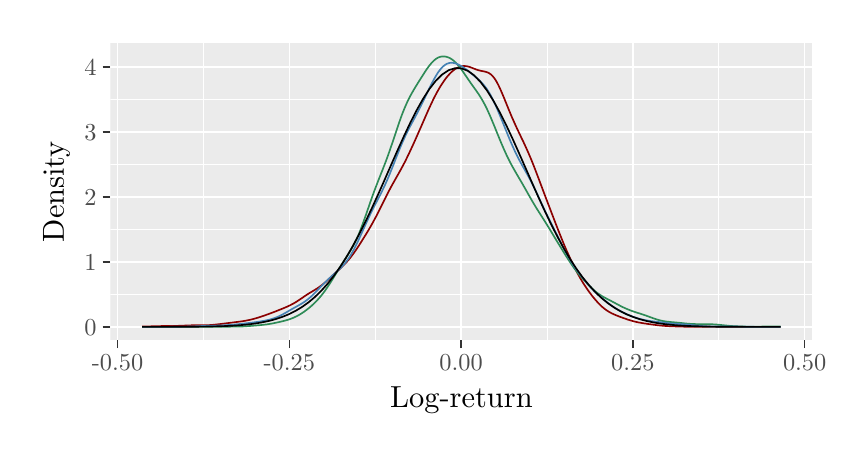
\begin{tikzpicture}[x=1pt,y=1pt]
\definecolor{fillColor}{RGB}{255,255,255}
\path[use as bounding box,fill=fillColor,fill opacity=0.00] (0,0) rectangle (289.08,144.54);
\begin{scope}
\path[clip] (  0.00,  0.00) rectangle (289.08,144.54);
\definecolor{drawColor}{RGB}{255,255,255}
\definecolor{fillColor}{RGB}{255,255,255}

\path[draw=drawColor,line width= 0.6pt,line join=round,line cap=round,fill=fillColor] (  0.00,  0.00) rectangle (289.08,144.54);
\end{scope}
\begin{scope}
\path[clip] ( 29.87, 31.53) rectangle (283.58,139.04);
\definecolor{fillColor}{gray}{0.92}

\path[fill=fillColor] ( 29.87, 31.53) rectangle (283.58,139.04);
\definecolor{drawColor}{RGB}{255,255,255}

\path[draw=drawColor,line width= 0.3pt,line join=round] ( 29.87, 48.14) --
	(283.58, 48.14);

\path[draw=drawColor,line width= 0.3pt,line join=round] ( 29.87, 71.59) --
	(283.58, 71.59);

\path[draw=drawColor,line width= 0.3pt,line join=round] ( 29.87, 95.04) --
	(283.58, 95.04);

\path[draw=drawColor,line width= 0.3pt,line join=round] ( 29.87,118.49) --
	(283.58,118.49);

\path[draw=drawColor,line width= 0.3pt,line join=round] ( 63.51, 31.53) --
	( 63.51,139.04);

\path[draw=drawColor,line width= 0.3pt,line join=round] (125.58, 31.53) --
	(125.58,139.04);

\path[draw=drawColor,line width= 0.3pt,line join=round] (187.65, 31.53) --
	(187.65,139.04);

\path[draw=drawColor,line width= 0.3pt,line join=round] (249.72, 31.53) --
	(249.72,139.04);

\path[draw=drawColor,line width= 0.6pt,line join=round] ( 29.87, 36.42) --
	(283.58, 36.42);

\path[draw=drawColor,line width= 0.6pt,line join=round] ( 29.87, 59.87) --
	(283.58, 59.87);

\path[draw=drawColor,line width= 0.6pt,line join=round] ( 29.87, 83.32) --
	(283.58, 83.32);

\path[draw=drawColor,line width= 0.6pt,line join=round] ( 29.87,106.77) --
	(283.58,106.77);

\path[draw=drawColor,line width= 0.6pt,line join=round] ( 29.87,130.22) --
	(283.58,130.22);

\path[draw=drawColor,line width= 0.6pt,line join=round] ( 32.48, 31.53) --
	( 32.48,139.04);

\path[draw=drawColor,line width= 0.6pt,line join=round] ( 94.55, 31.53) --
	( 94.55,139.04);

\path[draw=drawColor,line width= 0.6pt,line join=round] (156.62, 31.53) --
	(156.62,139.04);

\path[draw=drawColor,line width= 0.6pt,line join=round] (218.69, 31.53) --
	(218.69,139.04);

\path[draw=drawColor,line width= 0.6pt,line join=round] (280.76, 31.53) --
	(280.76,139.04);
\definecolor{drawColor}{RGB}{139,0,0}

\path[draw=drawColor,line width= 0.6pt,line join=round] ( 41.40, 36.54) --
	( 41.85, 36.55) --
	( 42.30, 36.56) --
	( 42.76, 36.57) --
	( 43.21, 36.58) --
	( 43.66, 36.60) --
	( 44.11, 36.61) --
	( 44.56, 36.62) --
	( 45.01, 36.63) --
	( 45.46, 36.64) --
	( 45.91, 36.66) --
	( 46.37, 36.67) --
	( 46.82, 36.68) --
	( 47.27, 36.69) --
	( 47.72, 36.70) --
	( 48.17, 36.71) --
	( 48.62, 36.72) --
	( 49.07, 36.73) --
	( 49.53, 36.74) --
	( 49.98, 36.74) --
	( 50.43, 36.75) --
	( 50.88, 36.75) --
	( 51.33, 36.75) --
	( 51.78, 36.76) --
	( 52.23, 36.76) --
	( 52.69, 36.77) --
	( 53.14, 36.77) --
	( 53.59, 36.78) --
	( 54.04, 36.79) --
	( 54.49, 36.80) --
	( 54.94, 36.82) --
	( 55.39, 36.83) --
	( 55.84, 36.85) --
	( 56.30, 36.87) --
	( 56.75, 36.89) --
	( 57.20, 36.91) --
	( 57.65, 36.93) --
	( 58.10, 36.95) --
	( 58.55, 36.96) --
	( 59.00, 36.98) --
	( 59.46, 36.99) --
	( 59.91, 36.99) --
	( 60.36, 36.99) --
	( 60.81, 37.00) --
	( 61.26, 36.99) --
	( 61.71, 36.99) --
	( 62.16, 36.99) --
	( 62.62, 36.99) --
	( 63.07, 36.99) --
	( 63.52, 36.99) --
	( 63.97, 37.00) --
	( 64.42, 37.01) --
	( 64.87, 37.03) --
	( 65.32, 37.05) --
	( 65.77, 37.07) --
	( 66.23, 37.10) --
	( 66.68, 37.14) --
	( 67.13, 37.18) --
	( 67.58, 37.22) --
	( 68.03, 37.27) --
	( 68.48, 37.32) --
	( 68.93, 37.37) --
	( 69.39, 37.42) --
	( 69.84, 37.48) --
	( 70.29, 37.53) --
	( 70.74, 37.59) --
	( 71.19, 37.64) --
	( 71.64, 37.70) --
	( 72.09, 37.76) --
	( 72.55, 37.81) --
	( 73.00, 37.87) --
	( 73.45, 37.93) --
	( 73.90, 37.98) --
	( 74.35, 38.04) --
	( 74.80, 38.10) --
	( 75.25, 38.15) --
	( 75.70, 38.21) --
	( 76.16, 38.27) --
	( 76.61, 38.33) --
	( 77.06, 38.39) --
	( 77.51, 38.45) --
	( 77.96, 38.52) --
	( 78.41, 38.60) --
	( 78.86, 38.68) --
	( 79.32, 38.76) --
	( 79.77, 38.85) --
	( 80.22, 38.95) --
	( 80.67, 39.06) --
	( 81.12, 39.17) --
	( 81.57, 39.28) --
	( 82.02, 39.41) --
	( 82.48, 39.54) --
	( 82.93, 39.67) --
	( 83.38, 39.81) --
	( 83.83, 39.95) --
	( 84.28, 40.10) --
	( 84.73, 40.25) --
	( 85.18, 40.41) --
	( 85.63, 40.56) --
	( 86.09, 40.72) --
	( 86.54, 40.88) --
	( 86.99, 41.04) --
	( 87.44, 41.21) --
	( 87.89, 41.38) --
	( 88.34, 41.55) --
	( 88.79, 41.72) --
	( 89.25, 41.89) --
	( 89.70, 42.07) --
	( 90.15, 42.24) --
	( 90.60, 42.42) --
	( 91.05, 42.60) --
	( 91.50, 42.78) --
	( 91.95, 42.97) --
	( 92.41, 43.15) --
	( 92.86, 43.34) --
	( 93.31, 43.54) --
	( 93.76, 43.73) --
	( 94.21, 43.94) --
	( 94.66, 44.15) --
	( 95.11, 44.37) --
	( 95.56, 44.61) --
	( 96.02, 44.86) --
	( 96.47, 45.11) --
	( 96.92, 45.39) --
	( 97.37, 45.67) --
	( 97.82, 45.96) --
	( 98.27, 46.26) --
	( 98.72, 46.57) --
	( 99.18, 46.88) --
	( 99.63, 47.19) --
	(100.08, 47.50) --
	(100.53, 47.80) --
	(100.98, 48.10) --
	(101.43, 48.39) --
	(101.88, 48.67) --
	(102.34, 48.94) --
	(102.79, 49.21) --
	(103.24, 49.48) --
	(103.69, 49.75) --
	(104.14, 50.02) --
	(104.59, 50.31) --
	(105.04, 50.60) --
	(105.49, 50.92) --
	(105.95, 51.24) --
	(106.40, 51.59) --
	(106.85, 51.95) --
	(107.30, 52.33) --
	(107.75, 52.72) --
	(108.20, 53.12) --
	(108.65, 53.54) --
	(109.11, 53.95) --
	(109.56, 54.38) --
	(110.01, 54.80) --
	(110.46, 55.22) --
	(110.91, 55.64) --
	(111.36, 56.06) --
	(111.81, 56.48) --
	(112.27, 56.90) --
	(112.72, 57.32) --
	(113.17, 57.74) --
	(113.62, 58.17) --
	(114.07, 58.62) --
	(114.52, 59.07) --
	(114.97, 59.54) --
	(115.42, 60.04) --
	(115.88, 60.55) --
	(116.33, 61.09) --
	(116.78, 61.66) --
	(117.23, 62.25) --
	(117.68, 62.86) --
	(118.13, 63.49) --
	(118.58, 64.15) --
	(119.04, 64.82) --
	(119.49, 65.51) --
	(119.94, 66.20) --
	(120.39, 66.91) --
	(120.84, 67.63) --
	(121.29, 68.35) --
	(121.74, 69.08) --
	(122.20, 69.81) --
	(122.65, 70.56) --
	(123.10, 71.31) --
	(123.55, 72.07) --
	(124.00, 72.85) --
	(124.45, 73.64) --
	(124.90, 74.46) --
	(125.35, 75.29) --
	(125.81, 76.14) --
	(126.26, 77.01) --
	(126.71, 77.90) --
	(127.16, 78.80) --
	(127.61, 79.71) --
	(128.06, 80.63) --
	(128.51, 81.54) --
	(128.97, 82.45) --
	(129.42, 83.36) --
	(129.87, 84.25) --
	(130.32, 85.12) --
	(130.77, 85.98) --
	(131.22, 86.83) --
	(131.67, 87.66) --
	(132.13, 88.47) --
	(132.58, 89.27) --
	(133.03, 90.07) --
	(133.48, 90.86) --
	(133.93, 91.66) --
	(134.38, 92.46) --
	(134.83, 93.27) --
	(135.28, 94.10) --
	(135.74, 94.95) --
	(136.19, 95.82) --
	(136.64, 96.71) --
	(137.09, 97.63) --
	(137.54, 98.56) --
	(137.99, 99.51) --
	(138.44,100.47) --
	(138.90,101.45) --
	(139.35,102.44) --
	(139.80,103.43) --
	(140.25,104.44) --
	(140.70,105.46) --
	(141.15,106.48) --
	(141.60,107.51) --
	(142.06,108.54) --
	(142.51,109.57) --
	(142.96,110.61) --
	(143.41,111.64) --
	(143.86,112.68) --
	(144.31,113.70) --
	(144.76,114.72) --
	(145.21,115.72) --
	(145.67,116.70) --
	(146.12,117.66) --
	(146.57,118.59) --
	(147.02,119.49) --
	(147.47,120.37) --
	(147.92,121.21) --
	(148.37,122.02) --
	(148.83,122.80) --
	(149.28,123.54) --
	(149.73,124.25) --
	(150.18,124.92) --
	(150.63,125.57) --
	(151.08,126.18) --
	(151.53,126.75) --
	(151.99,127.29) --
	(152.44,127.79) --
	(152.89,128.26) --
	(153.34,128.68) --
	(153.79,129.07) --
	(154.24,129.42) --
	(154.69,129.73) --
	(155.14,129.99) --
	(155.60,130.22) --
	(156.05,130.40) --
	(156.50,130.54) --
	(156.95,130.63) --
	(157.40,130.68) --
	(157.85,130.69) --
	(158.30,130.65) --
	(158.76,130.58) --
	(159.21,130.48) --
	(159.66,130.35) --
	(160.11,130.19) --
	(160.56,130.02) --
	(161.01,129.84) --
	(161.46,129.66) --
	(161.92,129.49) --
	(162.37,129.33) --
	(162.82,129.19) --
	(163.27,129.07) --
	(163.72,128.96) --
	(164.17,128.87) --
	(164.62,128.78) --
	(165.07,128.69) --
	(165.53,128.58) --
	(165.98,128.44) --
	(166.43,128.25) --
	(166.88,128.00) --
	(167.33,127.68) --
	(167.78,127.28) --
	(168.23,126.78) --
	(168.69,126.20) --
	(169.14,125.52) --
	(169.59,124.74) --
	(170.04,123.88) --
	(170.49,122.95) --
	(170.94,121.96) --
	(171.39,120.92) --
	(171.85,119.84) --
	(172.30,118.74) --
	(172.75,117.63) --
	(173.20,116.51) --
	(173.65,115.40) --
	(174.10,114.30) --
	(174.55,113.22) --
	(175.00,112.15) --
	(175.46,111.12) --
	(175.91,110.10) --
	(176.36,109.10) --
	(176.81,108.13) --
	(177.26,107.17) --
	(177.71,106.22) --
	(178.16,105.28) --
	(178.62,104.34) --
	(179.07,103.39) --
	(179.52,102.43) --
	(179.97,101.45) --
	(180.42,100.46) --
	(180.87, 99.44) --
	(181.32, 98.39) --
	(181.78, 97.32) --
	(182.23, 96.22) --
	(182.68, 95.09) --
	(183.13, 93.94) --
	(183.58, 92.77) --
	(184.03, 91.59) --
	(184.48, 90.40) --
	(184.93, 89.20) --
	(185.39, 87.99) --
	(185.84, 86.79) --
	(186.29, 85.59) --
	(186.74, 84.39) --
	(187.19, 83.19) --
	(187.64, 82.00) --
	(188.09, 80.81) --
	(188.55, 79.63) --
	(189.00, 78.44) --
	(189.45, 77.26) --
	(189.90, 76.08) --
	(190.35, 74.90) --
	(190.80, 73.72) --
	(191.25, 72.56) --
	(191.71, 71.40) --
	(192.16, 70.25) --
	(192.61, 69.12) --
	(193.06, 68.00) --
	(193.51, 66.90) --
	(193.96, 65.82) --
	(194.41, 64.77) --
	(194.86, 63.73) --
	(195.32, 62.72) --
	(195.77, 61.72) --
	(196.22, 60.75) --
	(196.67, 59.79) --
	(197.12, 58.86) --
	(197.57, 57.95) --
	(198.02, 57.06) --
	(198.48, 56.20) --
	(198.93, 55.36) --
	(199.38, 54.54) --
	(199.83, 53.75) --
	(200.28, 52.99) --
	(200.73, 52.26) --
	(201.18, 51.55) --
	(201.64, 50.86) --
	(202.09, 50.19) --
	(202.54, 49.55) --
	(202.99, 48.93) --
	(203.44, 48.33) --
	(203.89, 47.74) --
	(204.34, 47.17) --
	(204.79, 46.62) --
	(205.25, 46.09) --
	(205.70, 45.57) --
	(206.15, 45.08) --
	(206.60, 44.61) --
	(207.05, 44.17) --
	(207.50, 43.75) --
	(207.95, 43.36) --
	(208.41, 42.99) --
	(208.86, 42.65) --
	(209.31, 42.33) --
	(209.76, 42.04) --
	(210.21, 41.77) --
	(210.66, 41.52) --
	(211.11, 41.29) --
	(211.57, 41.08) --
	(212.02, 40.87) --
	(212.47, 40.68) --
	(212.92, 40.50) --
	(213.37, 40.32) --
	(213.82, 40.14) --
	(214.27, 39.98) --
	(214.72, 39.81) --
	(215.18, 39.64) --
	(215.63, 39.48) --
	(216.08, 39.33) --
	(216.53, 39.17) --
	(216.98, 39.02) --
	(217.43, 38.88) --
	(217.88, 38.74) --
	(218.34, 38.61) --
	(218.79, 38.48) --
	(219.24, 38.36) --
	(219.69, 38.26) --
	(220.14, 38.16) --
	(220.59, 38.06) --
	(221.04, 37.97) --
	(221.50, 37.89) --
	(221.95, 37.82) --
	(222.40, 37.74) --
	(222.85, 37.67) --
	(223.30, 37.61) --
	(223.75, 37.54) --
	(224.20, 37.47) --
	(224.65, 37.41) --
	(225.11, 37.35) --
	(225.56, 37.29) --
	(226.01, 37.22) --
	(226.46, 37.16) --
	(226.91, 37.11) --
	(227.36, 37.05) --
	(227.81, 37.00) --
	(228.27, 36.95) --
	(228.72, 36.90) --
	(229.17, 36.86) --
	(229.62, 36.82) --
	(230.07, 36.78) --
	(230.52, 36.75) --
	(230.97, 36.72) --
	(231.43, 36.70) --
	(231.88, 36.67) --
	(232.33, 36.65) --
	(232.78, 36.63) --
	(233.23, 36.62) --
	(233.68, 36.60) --
	(234.13, 36.58) --
	(234.58, 36.57) --
	(235.04, 36.55) --
	(235.49, 36.54) --
	(235.94, 36.53) --
	(236.39, 36.51) --
	(236.84, 36.50) --
	(237.29, 36.49) --
	(237.74, 36.48) --
	(238.20, 36.47) --
	(238.65, 36.46) --
	(239.10, 36.45) --
	(239.55, 36.45) --
	(240.00, 36.44) --
	(240.45, 36.43) --
	(240.90, 36.43) --
	(241.35, 36.43) --
	(241.81, 36.43) --
	(242.26, 36.42) --
	(242.71, 36.42) --
	(243.16, 36.42) --
	(243.61, 36.42) --
	(244.06, 36.42) --
	(244.51, 36.42) --
	(244.97, 36.42) --
	(245.42, 36.42) --
	(245.87, 36.42) --
	(246.32, 36.42) --
	(246.77, 36.42) --
	(247.22, 36.42) --
	(247.67, 36.42) --
	(248.13, 36.42) --
	(248.58, 36.42) --
	(249.03, 36.42) --
	(249.48, 36.42) --
	(249.93, 36.42) --
	(250.38, 36.42) --
	(250.83, 36.42) --
	(251.28, 36.42) --
	(251.74, 36.42) --
	(252.19, 36.42) --
	(252.64, 36.42) --
	(253.09, 36.42) --
	(253.54, 36.42) --
	(253.99, 36.42) --
	(254.44, 36.42) --
	(254.90, 36.42) --
	(255.35, 36.42) --
	(255.80, 36.42) --
	(256.25, 36.42) --
	(256.70, 36.42) --
	(257.15, 36.42) --
	(257.60, 36.42) --
	(258.06, 36.42) --
	(258.51, 36.42) --
	(258.96, 36.42) --
	(259.41, 36.42) --
	(259.86, 36.42) --
	(260.31, 36.42) --
	(260.76, 36.42) --
	(261.21, 36.42) --
	(261.67, 36.42) --
	(262.12, 36.42) --
	(262.57, 36.42) --
	(263.02, 36.42) --
	(263.47, 36.42) --
	(263.92, 36.42) --
	(264.37, 36.42) --
	(264.83, 36.42) --
	(265.28, 36.42) --
	(265.73, 36.42) --
	(266.18, 36.42) --
	(266.63, 36.42) --
	(267.08, 36.42) --
	(267.53, 36.42) --
	(267.99, 36.42) --
	(268.44, 36.42) --
	(268.89, 36.42) --
	(269.34, 36.42) --
	(269.79, 36.42) --
	(270.24, 36.42) --
	(270.69, 36.42) --
	(271.14, 36.42) --
	(271.60, 36.42) --
	(272.05, 36.42);
\definecolor{drawColor}{RGB}{46,139,87}

\path[draw=drawColor,line width= 0.6pt,line join=round] ( 41.40, 36.42) --
	( 41.85, 36.42) --
	( 42.30, 36.42) --
	( 42.76, 36.42) --
	( 43.21, 36.42) --
	( 43.66, 36.42) --
	( 44.11, 36.42) --
	( 44.56, 36.42) --
	( 45.01, 36.42) --
	( 45.46, 36.42) --
	( 45.91, 36.42) --
	( 46.37, 36.42) --
	( 46.82, 36.42) --
	( 47.27, 36.42) --
	( 47.72, 36.42) --
	( 48.17, 36.42) --
	( 48.62, 36.42) --
	( 49.07, 36.42) --
	( 49.53, 36.42) --
	( 49.98, 36.42) --
	( 50.43, 36.42) --
	( 50.88, 36.42) --
	( 51.33, 36.42) --
	( 51.78, 36.42) --
	( 52.23, 36.42) --
	( 52.69, 36.42) --
	( 53.14, 36.42) --
	( 53.59, 36.42) --
	( 54.04, 36.42) --
	( 54.49, 36.42) --
	( 54.94, 36.42) --
	( 55.39, 36.42) --
	( 55.84, 36.42) --
	( 56.30, 36.42) --
	( 56.75, 36.42) --
	( 57.20, 36.42) --
	( 57.65, 36.42) --
	( 58.10, 36.42) --
	( 58.55, 36.42) --
	( 59.00, 36.42) --
	( 59.46, 36.42) --
	( 59.91, 36.42) --
	( 60.36, 36.42) --
	( 60.81, 36.42) --
	( 61.26, 36.42) --
	( 61.71, 36.42) --
	( 62.16, 36.42) --
	( 62.62, 36.42) --
	( 63.07, 36.42) --
	( 63.52, 36.42) --
	( 63.97, 36.42) --
	( 64.42, 36.42) --
	( 64.87, 36.42) --
	( 65.32, 36.42) --
	( 65.77, 36.42) --
	( 66.23, 36.43) --
	( 66.68, 36.43) --
	( 67.13, 36.43) --
	( 67.58, 36.43) --
	( 68.03, 36.44) --
	( 68.48, 36.44) --
	( 68.93, 36.45) --
	( 69.39, 36.45) --
	( 69.84, 36.46) --
	( 70.29, 36.46) --
	( 70.74, 36.47) --
	( 71.19, 36.47) --
	( 71.64, 36.48) --
	( 72.09, 36.48) --
	( 72.55, 36.49) --
	( 73.00, 36.49) --
	( 73.45, 36.50) --
	( 73.90, 36.50) --
	( 74.35, 36.50) --
	( 74.80, 36.51) --
	( 75.25, 36.51) --
	( 75.70, 36.52) --
	( 76.16, 36.53) --
	( 76.61, 36.54) --
	( 77.06, 36.56) --
	( 77.51, 36.57) --
	( 77.96, 36.59) --
	( 78.41, 36.62) --
	( 78.86, 36.65) --
	( 79.32, 36.68) --
	( 79.77, 36.71) --
	( 80.22, 36.74) --
	( 80.67, 36.78) --
	( 81.12, 36.82) --
	( 81.57, 36.85) --
	( 82.02, 36.89) --
	( 82.48, 36.93) --
	( 82.93, 36.97) --
	( 83.38, 37.00) --
	( 83.83, 37.04) --
	( 84.28, 37.08) --
	( 84.73, 37.13) --
	( 85.18, 37.17) --
	( 85.63, 37.23) --
	( 86.09, 37.28) --
	( 86.54, 37.34) --
	( 86.99, 37.41) --
	( 87.44, 37.49) --
	( 87.89, 37.56) --
	( 88.34, 37.65) --
	( 88.79, 37.73) --
	( 89.25, 37.83) --
	( 89.70, 37.92) --
	( 90.15, 38.02) --
	( 90.60, 38.12) --
	( 91.05, 38.22) --
	( 91.50, 38.32) --
	( 91.95, 38.43) --
	( 92.41, 38.54) --
	( 92.86, 38.66) --
	( 93.31, 38.78) --
	( 93.76, 38.91) --
	( 94.21, 39.05) --
	( 94.66, 39.20) --
	( 95.11, 39.36) --
	( 95.56, 39.53) --
	( 96.02, 39.72) --
	( 96.47, 39.92) --
	( 96.92, 40.13) --
	( 97.37, 40.36) --
	( 97.82, 40.60) --
	( 98.27, 40.86) --
	( 98.72, 41.14) --
	( 99.18, 41.42) --
	( 99.63, 41.73) --
	(100.08, 42.04) --
	(100.53, 42.37) --
	(100.98, 42.72) --
	(101.43, 43.07) --
	(101.88, 43.44) --
	(102.34, 43.83) --
	(102.79, 44.23) --
	(103.24, 44.65) --
	(103.69, 45.08) --
	(104.14, 45.54) --
	(104.59, 46.01) --
	(105.04, 46.50) --
	(105.49, 47.01) --
	(105.95, 47.55) --
	(106.40, 48.11) --
	(106.85, 48.69) --
	(107.30, 49.30) --
	(107.75, 49.94) --
	(108.20, 50.59) --
	(108.65, 51.27) --
	(109.11, 51.96) --
	(109.56, 52.67) --
	(110.01, 53.39) --
	(110.46, 54.12) --
	(110.91, 54.86) --
	(111.36, 55.59) --
	(111.81, 56.33) --
	(112.27, 57.06) --
	(112.72, 57.78) --
	(113.17, 58.50) --
	(113.62, 59.21) --
	(114.07, 59.92) --
	(114.52, 60.61) --
	(114.97, 61.31) --
	(115.42, 62.01) --
	(115.88, 62.72) --
	(116.33, 63.45) --
	(116.78, 64.20) --
	(117.23, 64.99) --
	(117.68, 65.81) --
	(118.13, 66.67) --
	(118.58, 67.59) --
	(119.04, 68.56) --
	(119.49, 69.59) --
	(119.94, 70.68) --
	(120.39, 71.83) --
	(120.84, 73.02) --
	(121.29, 74.25) --
	(121.74, 75.52) --
	(122.20, 76.81) --
	(122.65, 78.12) --
	(123.10, 79.43) --
	(123.55, 80.74) --
	(124.00, 82.04) --
	(124.45, 83.31) --
	(124.90, 84.56) --
	(125.35, 85.79) --
	(125.81, 86.99) --
	(126.26, 88.17) --
	(126.71, 89.32) --
	(127.16, 90.47) --
	(127.61, 91.60) --
	(128.06, 92.74) --
	(128.51, 93.89) --
	(128.97, 95.05) --
	(129.42, 96.24) --
	(129.87, 97.45) --
	(130.32, 98.70) --
	(130.77, 99.97) --
	(131.22,101.28) --
	(131.67,102.61) --
	(132.13,103.96) --
	(132.58,105.32) --
	(133.03,106.68) --
	(133.48,108.04) --
	(133.93,109.37) --
	(134.38,110.67) --
	(134.83,111.94) --
	(135.28,113.17) --
	(135.74,114.34) --
	(136.19,115.45) --
	(136.64,116.50) --
	(137.09,117.50) --
	(137.54,118.45) --
	(137.99,119.35) --
	(138.44,120.20) --
	(138.90,121.02) --
	(139.35,121.80) --
	(139.80,122.57) --
	(140.25,123.31) --
	(140.70,124.04) --
	(141.15,124.77) --
	(141.60,125.49) --
	(142.06,126.21) --
	(142.51,126.92) --
	(142.96,127.63) --
	(143.41,128.33) --
	(143.86,129.01) --
	(144.31,129.68) --
	(144.76,130.31) --
	(145.21,130.91) --
	(145.67,131.47) --
	(146.12,131.98) --
	(146.57,132.44) --
	(147.02,132.85) --
	(147.47,133.21) --
	(147.92,133.51) --
	(148.37,133.75) --
	(148.83,133.93) --
	(149.28,134.05) --
	(149.73,134.13) --
	(150.18,134.15) --
	(150.63,134.13) --
	(151.08,134.06) --
	(151.53,133.95) --
	(151.99,133.80) --
	(152.44,133.60) --
	(152.89,133.35) --
	(153.34,133.05) --
	(153.79,132.71) --
	(154.24,132.32) --
	(154.69,131.89) --
	(155.14,131.41) --
	(155.60,130.89) --
	(156.05,130.34) --
	(156.50,129.75) --
	(156.95,129.13) --
	(157.40,128.48) --
	(157.85,127.82) --
	(158.30,127.16) --
	(158.76,126.49) --
	(159.21,125.83) --
	(159.66,125.17) --
	(160.11,124.52) --
	(160.56,123.89) --
	(161.01,123.25) --
	(161.46,122.63) --
	(161.92,122.00) --
	(162.37,121.36) --
	(162.82,120.70) --
	(163.27,120.02) --
	(163.72,119.30) --
	(164.17,118.55) --
	(164.62,117.76) --
	(165.07,116.93) --
	(165.53,116.04) --
	(165.98,115.11) --
	(166.43,114.14) --
	(166.88,113.13) --
	(167.33,112.09) --
	(167.78,111.02) --
	(168.23,109.93) --
	(168.69,108.83) --
	(169.14,107.72) --
	(169.59,106.60) --
	(170.04,105.49) --
	(170.49,104.38) --
	(170.94,103.29) --
	(171.39,102.22) --
	(171.85,101.17) --
	(172.30,100.15) --
	(172.75, 99.15) --
	(173.20, 98.18) --
	(173.65, 97.25) --
	(174.10, 96.35) --
	(174.55, 95.49) --
	(175.00, 94.64) --
	(175.46, 93.83) --
	(175.91, 93.03) --
	(176.36, 92.25) --
	(176.81, 91.47) --
	(177.26, 90.70) --
	(177.71, 89.94) --
	(178.16, 89.17) --
	(178.62, 88.39) --
	(179.07, 87.60) --
	(179.52, 86.81) --
	(179.97, 86.02) --
	(180.42, 85.22) --
	(180.87, 84.42) --
	(181.32, 83.62) --
	(181.78, 82.83) --
	(182.23, 82.04) --
	(182.68, 81.27) --
	(183.13, 80.52) --
	(183.58, 79.77) --
	(184.03, 79.04) --
	(184.48, 78.32) --
	(184.93, 77.61) --
	(185.39, 76.90) --
	(185.84, 76.19) --
	(186.29, 75.49) --
	(186.74, 74.77) --
	(187.19, 74.06) --
	(187.64, 73.33) --
	(188.09, 72.60) --
	(188.55, 71.86) --
	(189.00, 71.12) --
	(189.45, 70.37) --
	(189.90, 69.62) --
	(190.35, 68.87) --
	(190.80, 68.12) --
	(191.25, 67.37) --
	(191.71, 66.63) --
	(192.16, 65.89) --
	(192.61, 65.15) --
	(193.06, 64.42) --
	(193.51, 63.69) --
	(193.96, 62.96) --
	(194.41, 62.24) --
	(194.86, 61.53) --
	(195.32, 60.83) --
	(195.77, 60.14) --
	(196.22, 59.46) --
	(196.67, 58.79) --
	(197.12, 58.15) --
	(197.57, 57.52) --
	(198.02, 56.91) --
	(198.48, 56.32) --
	(198.93, 55.75) --
	(199.38, 55.20) --
	(199.83, 54.67) --
	(200.28, 54.15) --
	(200.73, 53.64) --
	(201.18, 53.14) --
	(201.64, 52.65) --
	(202.09, 52.18) --
	(202.54, 51.71) --
	(202.99, 51.24) --
	(203.44, 50.80) --
	(203.89, 50.36) --
	(204.34, 49.94) --
	(204.79, 49.54) --
	(205.25, 49.16) --
	(205.70, 48.80) --
	(206.15, 48.46) --
	(206.60, 48.14) --
	(207.05, 47.84) --
	(207.50, 47.56) --
	(207.95, 47.30) --
	(208.41, 47.05) --
	(208.86, 46.81) --
	(209.31, 46.57) --
	(209.76, 46.34) --
	(210.21, 46.10) --
	(210.66, 45.87) --
	(211.11, 45.63) --
	(211.57, 45.39) --
	(212.02, 45.15) --
	(212.47, 44.91) --
	(212.92, 44.66) --
	(213.37, 44.42) --
	(213.82, 44.19) --
	(214.27, 43.95) --
	(214.72, 43.72) --
	(215.18, 43.50) --
	(215.63, 43.29) --
	(216.08, 43.08) --
	(216.53, 42.89) --
	(216.98, 42.70) --
	(217.43, 42.52) --
	(217.88, 42.34) --
	(218.34, 42.18) --
	(218.79, 42.02) --
	(219.24, 41.87) --
	(219.69, 41.72) --
	(220.14, 41.57) --
	(220.59, 41.43) --
	(221.04, 41.29) --
	(221.50, 41.14) --
	(221.95, 41.00) --
	(222.40, 40.85) --
	(222.85, 40.70) --
	(223.30, 40.54) --
	(223.75, 40.38) --
	(224.20, 40.22) --
	(224.65, 40.05) --
	(225.11, 39.89) --
	(225.56, 39.72) --
	(226.01, 39.56) --
	(226.46, 39.40) --
	(226.91, 39.25) --
	(227.36, 39.10) --
	(227.81, 38.97) --
	(228.27, 38.84) --
	(228.72, 38.73) --
	(229.17, 38.63) --
	(229.62, 38.53) --
	(230.07, 38.46) --
	(230.52, 38.39) --
	(230.97, 38.32) --
	(231.43, 38.27) --
	(231.88, 38.22) --
	(232.33, 38.18) --
	(232.78, 38.14) --
	(233.23, 38.10) --
	(233.68, 38.06) --
	(234.13, 38.02) --
	(234.58, 37.98) --
	(235.04, 37.94) --
	(235.49, 37.89) --
	(235.94, 37.84) --
	(236.39, 37.80) --
	(236.84, 37.75) --
	(237.29, 37.70) --
	(237.74, 37.66) --
	(238.20, 37.61) --
	(238.65, 37.57) --
	(239.10, 37.54) --
	(239.55, 37.51) --
	(240.00, 37.48) --
	(240.45, 37.46) --
	(240.90, 37.44) --
	(241.35, 37.43) --
	(241.81, 37.42) --
	(242.26, 37.42) --
	(242.71, 37.42) --
	(243.16, 37.42) --
	(243.61, 37.42) --
	(244.06, 37.42) --
	(244.51, 37.42) --
	(244.97, 37.42) --
	(245.42, 37.42) --
	(245.87, 37.41) --
	(246.32, 37.40) --
	(246.77, 37.39) --
	(247.22, 37.37) --
	(247.67, 37.34) --
	(248.13, 37.32) --
	(248.58, 37.28) --
	(249.03, 37.25) --
	(249.48, 37.20) --
	(249.93, 37.16) --
	(250.38, 37.12) --
	(250.83, 37.07) --
	(251.28, 37.02) --
	(251.74, 36.98) --
	(252.19, 36.93) --
	(252.64, 36.89) --
	(253.09, 36.84) --
	(253.54, 36.80) --
	(253.99, 36.77) --
	(254.44, 36.73) --
	(254.90, 36.70) --
	(255.35, 36.68) --
	(255.80, 36.65) --
	(256.25, 36.63) --
	(256.70, 36.61) --
	(257.15, 36.59) --
	(257.60, 36.57) --
	(258.06, 36.56) --
	(258.51, 36.55) --
	(258.96, 36.54) --
	(259.41, 36.53) --
	(259.86, 36.52) --
	(260.31, 36.52) --
	(260.76, 36.51) --
	(261.21, 36.51) --
	(261.67, 36.51) --
	(262.12, 36.51) --
	(262.57, 36.51) --
	(263.02, 36.51) --
	(263.47, 36.51) --
	(263.92, 36.52) --
	(264.37, 36.52) --
	(264.83, 36.52) --
	(265.28, 36.53) --
	(265.73, 36.54) --
	(266.18, 36.54) --
	(266.63, 36.55) --
	(267.08, 36.55) --
	(267.53, 36.55) --
	(267.99, 36.56) --
	(268.44, 36.56) --
	(268.89, 36.56) --
	(269.34, 36.57) --
	(269.79, 36.57) --
	(270.24, 36.57) --
	(270.69, 36.56) --
	(271.14, 36.56) --
	(271.60, 36.55) --
	(272.05, 36.55);
\definecolor{drawColor}{RGB}{70,130,180}

\path[draw=drawColor,line width= 0.6pt,line join=round] ( 41.40, 36.42) --
	( 41.85, 36.42) --
	( 42.30, 36.42) --
	( 42.76, 36.42) --
	( 43.21, 36.42) --
	( 43.66, 36.42) --
	( 44.11, 36.42) --
	( 44.56, 36.42) --
	( 45.01, 36.42) --
	( 45.46, 36.42) --
	( 45.91, 36.42) --
	( 46.37, 36.42) --
	( 46.82, 36.42) --
	( 47.27, 36.42) --
	( 47.72, 36.42) --
	( 48.17, 36.42) --
	( 48.62, 36.42) --
	( 49.07, 36.42) --
	( 49.53, 36.43) --
	( 49.98, 36.43) --
	( 50.43, 36.43) --
	( 50.88, 36.43) --
	( 51.33, 36.44) --
	( 51.78, 36.44) --
	( 52.23, 36.45) --
	( 52.69, 36.45) --
	( 53.14, 36.46) --
	( 53.59, 36.46) --
	( 54.04, 36.47) --
	( 54.49, 36.48) --
	( 54.94, 36.49) --
	( 55.39, 36.49) --
	( 55.84, 36.50) --
	( 56.30, 36.51) --
	( 56.75, 36.52) --
	( 57.20, 36.52) --
	( 57.65, 36.53) --
	( 58.10, 36.54) --
	( 58.55, 36.56) --
	( 59.00, 36.57) --
	( 59.46, 36.58) --
	( 59.91, 36.60) --
	( 60.36, 36.61) --
	( 60.81, 36.63) --
	( 61.26, 36.65) --
	( 61.71, 36.67) --
	( 62.16, 36.69) --
	( 62.62, 36.71) --
	( 63.07, 36.73) --
	( 63.52, 36.75) --
	( 63.97, 36.76) --
	( 64.42, 36.78) --
	( 64.87, 36.80) --
	( 65.32, 36.81) --
	( 65.77, 36.82) --
	( 66.23, 36.83) --
	( 66.68, 36.84) --
	( 67.13, 36.85) --
	( 67.58, 36.86) --
	( 68.03, 36.88) --
	( 68.48, 36.89) --
	( 68.93, 36.90) --
	( 69.39, 36.92) --
	( 69.84, 36.93) --
	( 70.29, 36.95) --
	( 70.74, 36.98) --
	( 71.19, 37.00) --
	( 71.64, 37.03) --
	( 72.09, 37.06) --
	( 72.55, 37.09) --
	( 73.00, 37.13) --
	( 73.45, 37.16) --
	( 73.90, 37.20) --
	( 74.35, 37.24) --
	( 74.80, 37.28) --
	( 75.25, 37.32) --
	( 75.70, 37.37) --
	( 76.16, 37.41) --
	( 76.61, 37.46) --
	( 77.06, 37.51) --
	( 77.51, 37.55) --
	( 77.96, 37.60) --
	( 78.41, 37.65) --
	( 78.86, 37.71) --
	( 79.32, 37.76) --
	( 79.77, 37.81) --
	( 80.22, 37.87) --
	( 80.67, 37.92) --
	( 81.12, 37.98) --
	( 81.57, 38.03) --
	( 82.02, 38.09) --
	( 82.48, 38.15) --
	( 82.93, 38.21) --
	( 83.38, 38.28) --
	( 83.83, 38.34) --
	( 84.28, 38.42) --
	( 84.73, 38.49) --
	( 85.18, 38.57) --
	( 85.63, 38.66) --
	( 86.09, 38.75) --
	( 86.54, 38.84) --
	( 86.99, 38.95) --
	( 87.44, 39.06) --
	( 87.89, 39.19) --
	( 88.34, 39.32) --
	( 88.79, 39.47) --
	( 89.25, 39.62) --
	( 89.70, 39.79) --
	( 90.15, 39.98) --
	( 90.60, 40.17) --
	( 91.05, 40.38) --
	( 91.50, 40.60) --
	( 91.95, 40.84) --
	( 92.41, 41.08) --
	( 92.86, 41.33) --
	( 93.31, 41.58) --
	( 93.76, 41.84) --
	( 94.21, 42.11) --
	( 94.66, 42.37) --
	( 95.11, 42.63) --
	( 95.56, 42.89) --
	( 96.02, 43.15) --
	( 96.47, 43.40) --
	( 96.92, 43.65) --
	( 97.37, 43.90) --
	( 97.82, 44.15) --
	( 98.27, 44.41) --
	( 98.72, 44.67) --
	( 99.18, 44.94) --
	( 99.63, 45.23) --
	(100.08, 45.53) --
	(100.53, 45.85) --
	(100.98, 46.18) --
	(101.43, 46.54) --
	(101.88, 46.91) --
	(102.34, 47.31) --
	(102.79, 47.73) --
	(103.24, 48.16) --
	(103.69, 48.61) --
	(104.14, 49.07) --
	(104.59, 49.54) --
	(105.04, 50.01) --
	(105.49, 50.48) --
	(105.95, 50.96) --
	(106.40, 51.42) --
	(106.85, 51.89) --
	(107.30, 52.34) --
	(107.75, 52.79) --
	(108.20, 53.23) --
	(108.65, 53.65) --
	(109.11, 54.07) --
	(109.56, 54.49) --
	(110.01, 54.90) --
	(110.46, 55.30) --
	(110.91, 55.70) --
	(111.36, 56.10) --
	(111.81, 56.51) --
	(112.27, 56.92) --
	(112.72, 57.35) --
	(113.17, 57.79) --
	(113.62, 58.25) --
	(114.07, 58.74) --
	(114.52, 59.26) --
	(114.97, 59.81) --
	(115.42, 60.41) --
	(115.88, 61.05) --
	(116.33, 61.73) --
	(116.78, 62.46) --
	(117.23, 63.23) --
	(117.68, 64.05) --
	(118.13, 64.90) --
	(118.58, 65.79) --
	(119.04, 66.71) --
	(119.49, 67.67) --
	(119.94, 68.64) --
	(120.39, 69.64) --
	(120.84, 70.64) --
	(121.29, 71.65) --
	(121.74, 72.65) --
	(122.20, 73.65) --
	(122.65, 74.64) --
	(123.10, 75.62) --
	(123.55, 76.58) --
	(124.00, 77.52) --
	(124.45, 78.44) --
	(124.90, 79.35) --
	(125.35, 80.23) --
	(125.81, 81.11) --
	(126.26, 81.98) --
	(126.71, 82.85) --
	(127.16, 83.72) --
	(127.61, 84.61) --
	(128.06, 85.51) --
	(128.51, 86.44) --
	(128.97, 87.40) --
	(129.42, 88.39) --
	(129.87, 89.41) --
	(130.32, 90.46) --
	(130.77, 91.54) --
	(131.22, 92.65) --
	(131.67, 93.78) --
	(132.13, 94.93) --
	(132.58, 96.09) --
	(133.03, 97.25) --
	(133.48, 98.40) --
	(133.93, 99.53) --
	(134.38,100.65) --
	(134.83,101.74) --
	(135.28,102.80) --
	(135.74,103.83) --
	(136.19,104.82) --
	(136.64,105.78) --
	(137.09,106.71) --
	(137.54,107.61) --
	(137.99,108.49) --
	(138.44,109.35) --
	(138.90,110.20) --
	(139.35,111.04) --
	(139.80,111.88) --
	(140.25,112.72) --
	(140.70,113.58) --
	(141.15,114.45) --
	(141.60,115.33) --
	(142.06,116.23) --
	(142.51,117.14) --
	(142.96,118.06) --
	(143.41,119.00) --
	(143.86,119.94) --
	(144.31,120.89) --
	(144.76,121.83) --
	(145.21,122.76) --
	(145.67,123.67) --
	(146.12,124.56) --
	(146.57,125.42) --
	(147.02,126.24) --
	(147.47,127.03) --
	(147.92,127.77) --
	(148.37,128.46) --
	(148.83,129.09) --
	(149.28,129.65) --
	(149.73,130.15) --
	(150.18,130.59) --
	(150.63,130.96) --
	(151.08,131.26) --
	(151.53,131.50) --
	(151.99,131.67) --
	(152.44,131.79) --
	(152.89,131.84) --
	(153.34,131.84) --
	(153.79,131.80) --
	(154.24,131.71) --
	(154.69,131.59) --
	(155.14,131.43) --
	(155.60,131.24) --
	(156.05,131.02) --
	(156.50,130.78) --
	(156.95,130.51) --
	(157.40,130.22) --
	(157.85,129.91) --
	(158.30,129.58) --
	(158.76,129.24) --
	(159.21,128.89) --
	(159.66,128.52) --
	(160.11,128.15) --
	(160.56,127.77) --
	(161.01,127.39) --
	(161.46,127.01) --
	(161.92,126.62) --
	(162.37,126.23) --
	(162.82,125.83) --
	(163.27,125.41) --
	(163.72,124.98) --
	(164.17,124.52) --
	(164.62,124.02) --
	(165.07,123.49) --
	(165.53,122.90) --
	(165.98,122.27) --
	(166.43,121.57) --
	(166.88,120.83) --
	(167.33,120.03) --
	(167.78,119.17) --
	(168.23,118.27) --
	(168.69,117.33) --
	(169.14,116.34) --
	(169.59,115.32) --
	(170.04,114.26) --
	(170.49,113.19) --
	(170.94,112.10) --
	(171.39,111.00) --
	(171.85,109.88) --
	(172.30,108.76) --
	(172.75,107.65) --
	(173.20,106.53) --
	(173.65,105.43) --
	(174.10,104.34) --
	(174.55,103.27) --
	(175.00,102.22) --
	(175.46,101.21) --
	(175.91,100.22) --
	(176.36, 99.26) --
	(176.81, 98.34) --
	(177.26, 97.45) --
	(177.71, 96.59) --
	(178.16, 95.75) --
	(178.62, 94.94) --
	(179.07, 94.13) --
	(179.52, 93.34) --
	(179.97, 92.54) --
	(180.42, 91.73) --
	(180.87, 90.91) --
	(181.32, 90.08) --
	(181.78, 89.22) --
	(182.23, 88.33) --
	(182.68, 87.42) --
	(183.13, 86.49) --
	(183.58, 85.54) --
	(184.03, 84.58) --
	(184.48, 83.60) --
	(184.93, 82.62) --
	(185.39, 81.64) --
	(185.84, 80.66) --
	(186.29, 79.70) --
	(186.74, 78.74) --
	(187.19, 77.80) --
	(187.64, 76.88) --
	(188.09, 75.96) --
	(188.55, 75.06) --
	(189.00, 74.17) --
	(189.45, 73.27) --
	(189.90, 72.38) --
	(190.35, 71.49) --
	(190.80, 70.59) --
	(191.25, 69.68) --
	(191.71, 68.78) --
	(192.16, 67.87) --
	(192.61, 66.96) --
	(193.06, 66.06) --
	(193.51, 65.17) --
	(193.96, 64.29) --
	(194.41, 63.43) --
	(194.86, 62.60) --
	(195.32, 61.80) --
	(195.77, 61.02) --
	(196.22, 60.27) --
	(196.67, 59.55) --
	(197.12, 58.85) --
	(197.57, 58.18) --
	(198.02, 57.53) --
	(198.48, 56.91) --
	(198.93, 56.29) --
	(199.38, 55.69) --
	(199.83, 55.10) --
	(200.28, 54.52) --
	(200.73, 53.95) --
	(201.18, 53.39) --
	(201.64, 52.83) --
	(202.09, 52.28) --
	(202.54, 51.75) --
	(202.99, 51.23) --
	(203.44, 50.72) --
	(203.89, 50.23) --
	(204.34, 49.75) --
	(204.79, 49.29) --
	(205.25, 48.85) --
	(205.70, 48.42) --
	(206.15, 48.01) --
	(206.60, 47.61) --
	(207.05, 47.22) --
	(207.50, 46.83) --
	(207.95, 46.46) --
	(208.41, 46.09) --
	(208.86, 45.73) --
	(209.31, 45.37) --
	(209.76, 45.02) --
	(210.21, 44.68) --
	(210.66, 44.35) --
	(211.11, 44.02) --
	(211.57, 43.71) --
	(212.02, 43.41) --
	(212.47, 43.12) --
	(212.92, 42.84) --
	(213.37, 42.57) --
	(213.82, 42.32) --
	(214.27, 42.07) --
	(214.72, 41.84) --
	(215.18, 41.61) --
	(215.63, 41.39) --
	(216.08, 41.18) --
	(216.53, 40.98) --
	(216.98, 40.78) --
	(217.43, 40.59) --
	(217.88, 40.41) --
	(218.34, 40.24) --
	(218.79, 40.07) --
	(219.24, 39.91) --
	(219.69, 39.75) --
	(220.14, 39.61) --
	(220.59, 39.47) --
	(221.04, 39.34) --
	(221.50, 39.22) --
	(221.95, 39.11) --
	(222.40, 39.01) --
	(222.85, 38.91) --
	(223.30, 38.83) --
	(223.75, 38.74) --
	(224.20, 38.67) --
	(224.65, 38.60) --
	(225.11, 38.53) --
	(225.56, 38.47) --
	(226.01, 38.42) --
	(226.46, 38.36) --
	(226.91, 38.30) --
	(227.36, 38.25) --
	(227.81, 38.20) --
	(228.27, 38.14) --
	(228.72, 38.09) --
	(229.17, 38.04) --
	(229.62, 37.98) --
	(230.07, 37.93) --
	(230.52, 37.87) --
	(230.97, 37.82) --
	(231.43, 37.77) --
	(231.88, 37.72) --
	(232.33, 37.68) --
	(232.78, 37.63) --
	(233.23, 37.59) --
	(233.68, 37.56) --
	(234.13, 37.52) --
	(234.58, 37.49) --
	(235.04, 37.46) --
	(235.49, 37.43) --
	(235.94, 37.40) --
	(236.39, 37.37) --
	(236.84, 37.35) --
	(237.29, 37.31) --
	(237.74, 37.28) --
	(238.20, 37.25) --
	(238.65, 37.21) --
	(239.10, 37.17) --
	(239.55, 37.13) --
	(240.00, 37.08) --
	(240.45, 37.04) --
	(240.90, 36.99) --
	(241.35, 36.94) --
	(241.81, 36.90) --
	(242.26, 36.85) --
	(242.71, 36.81) --
	(243.16, 36.77) --
	(243.61, 36.73) --
	(244.06, 36.70) --
	(244.51, 36.67) --
	(244.97, 36.64) --
	(245.42, 36.62) --
	(245.87, 36.60) --
	(246.32, 36.58) --
	(246.77, 36.57) --
	(247.22, 36.56) --
	(247.67, 36.55) --
	(248.13, 36.55) --
	(248.58, 36.54) --
	(249.03, 36.54) --
	(249.48, 36.54) --
	(249.93, 36.54) --
	(250.38, 36.54) --
	(250.83, 36.54) --
	(251.28, 36.54) --
	(251.74, 36.54) --
	(252.19, 36.55) --
	(252.64, 36.55) --
	(253.09, 36.55) --
	(253.54, 36.55) --
	(253.99, 36.55) --
	(254.44, 36.55) --
	(254.90, 36.54) --
	(255.35, 36.54) --
	(255.80, 36.54) --
	(256.25, 36.53) --
	(256.70, 36.53) --
	(257.15, 36.52) --
	(257.60, 36.51) --
	(258.06, 36.51) --
	(258.51, 36.50) --
	(258.96, 36.49) --
	(259.41, 36.48) --
	(259.86, 36.47) --
	(260.31, 36.47) --
	(260.76, 36.46) --
	(261.21, 36.45) --
	(261.67, 36.45) --
	(262.12, 36.44) --
	(262.57, 36.44) --
	(263.02, 36.43) --
	(263.47, 36.43) --
	(263.92, 36.43) --
	(264.37, 36.42) --
	(264.83, 36.42) --
	(265.28, 36.42) --
	(265.73, 36.42) --
	(266.18, 36.42) --
	(266.63, 36.42) --
	(267.08, 36.42) --
	(267.53, 36.42) --
	(267.99, 36.42) --
	(268.44, 36.42) --
	(268.89, 36.42) --
	(269.34, 36.42) --
	(269.79, 36.42) --
	(270.24, 36.42) --
	(270.69, 36.42) --
	(271.14, 36.42) --
	(271.60, 36.42) --
	(272.05, 36.42);
\definecolor{drawColor}{RGB}{0,0,0}

\path[draw=drawColor,line width= 0.6pt,line join=round] ( 41.40, 36.42) --
	( 43.71, 36.42) --
	( 46.01, 36.42) --
	( 48.32, 36.43) --
	( 50.63, 36.43) --
	( 52.93, 36.44) --
	( 55.24, 36.44) --
	( 57.55, 36.46) --
	( 59.85, 36.47) --
	( 62.16, 36.50) --
	( 64.47, 36.53) --
	( 66.77, 36.58) --
	( 69.08, 36.64) --
	( 71.39, 36.72) --
	( 73.69, 36.83) --
	( 76.00, 36.98) --
	( 78.30, 37.17) --
	( 80.61, 37.42) --
	( 82.92, 37.74) --
	( 85.22, 38.15) --
	( 87.53, 38.65) --
	( 89.84, 39.29) --
	( 92.14, 40.07) --
	( 94.45, 41.02) --
	( 96.76, 42.18) --
	( 99.06, 43.56) --
	(101.37, 45.20) --
	(103.68, 47.12) --
	(105.98, 49.35) --
	(108.29, 51.91) --
	(110.60, 54.81) --
	(112.90, 58.07) --
	(115.21, 61.69) --
	(117.51, 65.67) --
	(119.82, 69.97) --
	(122.13, 74.58) --
	(124.43, 79.45) --
	(126.74, 84.52) --
	(129.05, 89.73) --
	(131.35, 95.00) --
	(133.66,100.23) --
	(135.97,105.34) --
	(138.27,110.21) --
	(140.58,114.75) --
	(142.89,118.85) --
	(145.19,122.42) --
	(147.50,125.38) --
	(149.81,127.65) --
	(152.11,129.17) --
	(154.42,129.90) --
	(156.72,129.83) --
	(159.03,128.96) --
	(161.34,127.31) --
	(163.64,124.92) --
	(165.95,121.86) --
	(168.26,118.19) --
	(170.56,114.01) --
	(172.87,109.41) --
	(175.18,104.49) --
	(177.48, 99.35) --
	(179.79, 94.11) --
	(182.10, 88.84) --
	(184.40, 83.65) --
	(186.71, 78.61) --
	(189.01, 73.78) --
	(191.32, 69.22) --
	(193.63, 64.97) --
	(195.93, 61.05) --
	(198.24, 57.49) --
	(200.55, 54.29) --
	(202.85, 51.45) --
	(205.16, 48.95) --
	(207.47, 46.77) --
	(209.77, 44.90) --
	(212.08, 43.31) --
	(214.39, 41.97) --
	(216.69, 40.85) --
	(219.00, 39.93) --
	(221.31, 39.17) --
	(223.61, 38.56) --
	(225.92, 38.07) --
	(228.22, 37.68) --
	(230.53, 37.38) --
	(232.84, 37.14) --
	(235.14, 36.95) --
	(237.45, 36.81) --
	(239.76, 36.71) --
	(242.06, 36.63) --
	(244.37, 36.57) --
	(246.68, 36.53) --
	(248.98, 36.49) --
	(251.29, 36.47) --
	(253.60, 36.45) --
	(255.90, 36.44) --
	(258.21, 36.44) --
	(260.52, 36.43) --
	(262.82, 36.43) --
	(265.13, 36.42) --
	(267.43, 36.42) --
	(269.74, 36.42) --
	(272.05, 36.42);
\end{scope}
\begin{scope}
\path[clip] (  0.00,  0.00) rectangle (289.08,144.54);
\definecolor{drawColor}{gray}{0.30}

\node[text=drawColor,anchor=base east,inner sep=0pt, outer sep=0pt, scale=  0.88] at ( 24.92, 33.39) {0};

\node[text=drawColor,anchor=base east,inner sep=0pt, outer sep=0pt, scale=  0.88] at ( 24.92, 56.84) {1};

\node[text=drawColor,anchor=base east,inner sep=0pt, outer sep=0pt, scale=  0.88] at ( 24.92, 80.29) {2};

\node[text=drawColor,anchor=base east,inner sep=0pt, outer sep=0pt, scale=  0.88] at ( 24.92,103.74) {3};

\node[text=drawColor,anchor=base east,inner sep=0pt, outer sep=0pt, scale=  0.88] at ( 24.92,127.19) {4};
\end{scope}
\begin{scope}
\path[clip] (  0.00,  0.00) rectangle (289.08,144.54);
\definecolor{drawColor}{gray}{0.20}

\path[draw=drawColor,line width= 0.6pt,line join=round] ( 27.12, 36.42) --
	( 29.87, 36.42);

\path[draw=drawColor,line width= 0.6pt,line join=round] ( 27.12, 59.87) --
	( 29.87, 59.87);

\path[draw=drawColor,line width= 0.6pt,line join=round] ( 27.12, 83.32) --
	( 29.87, 83.32);

\path[draw=drawColor,line width= 0.6pt,line join=round] ( 27.12,106.77) --
	( 29.87,106.77);

\path[draw=drawColor,line width= 0.6pt,line join=round] ( 27.12,130.22) --
	( 29.87,130.22);
\end{scope}
\begin{scope}
\path[clip] (  0.00,  0.00) rectangle (289.08,144.54);
\definecolor{drawColor}{gray}{0.20}

\path[draw=drawColor,line width= 0.6pt,line join=round] ( 32.48, 28.78) --
	( 32.48, 31.53);

\path[draw=drawColor,line width= 0.6pt,line join=round] ( 94.55, 28.78) --
	( 94.55, 31.53);

\path[draw=drawColor,line width= 0.6pt,line join=round] (156.62, 28.78) --
	(156.62, 31.53);

\path[draw=drawColor,line width= 0.6pt,line join=round] (218.69, 28.78) --
	(218.69, 31.53);

\path[draw=drawColor,line width= 0.6pt,line join=round] (280.76, 28.78) --
	(280.76, 31.53);
\end{scope}
\begin{scope}
\path[clip] (  0.00,  0.00) rectangle (289.08,144.54);
\definecolor{drawColor}{gray}{0.30}

\node[text=drawColor,anchor=base,inner sep=0pt, outer sep=0pt, scale=  0.88] at ( 32.48, 20.52) {-0.50};

\node[text=drawColor,anchor=base,inner sep=0pt, outer sep=0pt, scale=  0.88] at ( 94.55, 20.52) {-0.25};

\node[text=drawColor,anchor=base,inner sep=0pt, outer sep=0pt, scale=  0.88] at (156.62, 20.52) {0.00};

\node[text=drawColor,anchor=base,inner sep=0pt, outer sep=0pt, scale=  0.88] at (218.69, 20.52) {0.25};

\node[text=drawColor,anchor=base,inner sep=0pt, outer sep=0pt, scale=  0.88] at (280.76, 20.52) {0.50};
\end{scope}
\begin{scope}
\path[clip] (  0.00,  0.00) rectangle (289.08,144.54);
\definecolor{drawColor}{RGB}{0,0,0}

\node[text=drawColor,anchor=base,inner sep=0pt, outer sep=0pt, scale=  1.10] at (156.72,  7.44) {Log-return};
\end{scope}
\begin{scope}
\path[clip] (  0.00,  0.00) rectangle (289.08,144.54);
\definecolor{drawColor}{RGB}{0,0,0}

\node[text=drawColor,rotate= 90.00,anchor=base,inner sep=0pt, outer sep=0pt, scale=  1.10] at ( 13.08, 85.29) {Density};
\end{scope}
\end{tikzpicture}

\end{figure}
\end{block}
\end{frame}

\begin{frame}{MJD: log-return density}
\begin{block}{Impact on the kurtosis}
\begin{figure}[ht]
\centering
% Created by tikzDevice version 0.11 on 2018-08-25 22:37:55
% !TEX encoding = UTF-8 Unicode
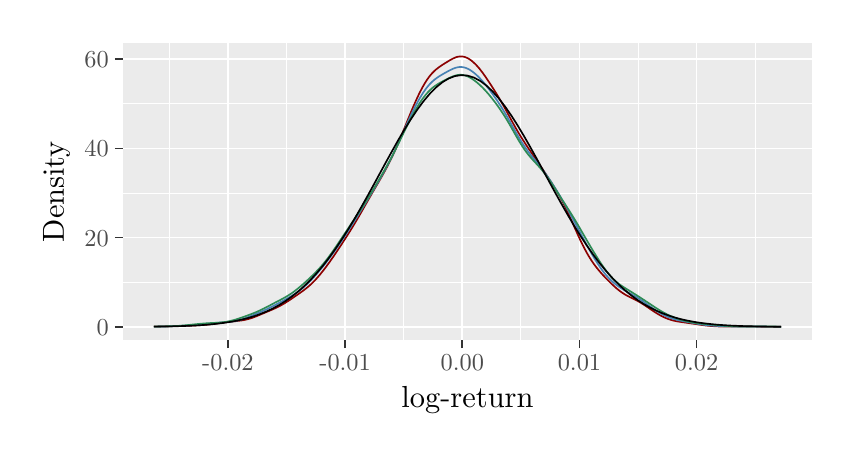
\begin{tikzpicture}[x=1pt,y=1pt]
\definecolor{fillColor}{RGB}{255,255,255}
\path[use as bounding box,fill=fillColor,fill opacity=0.00] (0,0) rectangle (289.08,144.54);
\begin{scope}
\path[clip] (  0.00,  0.00) rectangle (289.08,144.54);
\definecolor{drawColor}{RGB}{255,255,255}
\definecolor{fillColor}{RGB}{255,255,255}

\path[draw=drawColor,line width= 0.6pt,line join=round,line cap=round,fill=fillColor] (  0.00,  0.00) rectangle (289.08,144.54);
\end{scope}
\begin{scope}
\path[clip] ( 34.27, 31.53) rectangle (283.58,139.04);
\definecolor{fillColor}{gray}{0.92}

\path[fill=fillColor] ( 34.27, 31.53) rectangle (283.58,139.04);
\definecolor{drawColor}{RGB}{255,255,255}

\path[draw=drawColor,line width= 0.3pt,line join=round] ( 34.27, 52.54) --
	(283.58, 52.54);

\path[draw=drawColor,line width= 0.3pt,line join=round] ( 34.27, 84.80) --
	(283.58, 84.80);

\path[draw=drawColor,line width= 0.3pt,line join=round] ( 34.27,117.05) --
	(283.58,117.05);

\path[draw=drawColor,line width= 0.3pt,line join=round] ( 51.19, 31.53) --
	( 51.19,139.04);

\path[draw=drawColor,line width= 0.3pt,line join=round] ( 93.53, 31.53) --
	( 93.53,139.04);

\path[draw=drawColor,line width= 0.3pt,line join=round] (135.88, 31.53) --
	(135.88,139.04);

\path[draw=drawColor,line width= 0.3pt,line join=round] (178.22, 31.53) --
	(178.22,139.04);

\path[draw=drawColor,line width= 0.3pt,line join=round] (220.56, 31.53) --
	(220.56,139.04);

\path[draw=drawColor,line width= 0.3pt,line join=round] (262.90, 31.53) --
	(262.90,139.04);

\path[draw=drawColor,line width= 0.6pt,line join=round] ( 34.27, 36.42) --
	(283.58, 36.42);

\path[draw=drawColor,line width= 0.6pt,line join=round] ( 34.27, 68.67) --
	(283.58, 68.67);

\path[draw=drawColor,line width= 0.6pt,line join=round] ( 34.27,100.92) --
	(283.58,100.92);

\path[draw=drawColor,line width= 0.6pt,line join=round] ( 34.27,133.18) --
	(283.58,133.18);

\path[draw=drawColor,line width= 0.6pt,line join=round] ( 72.36, 31.53) --
	( 72.36,139.04);

\path[draw=drawColor,line width= 0.6pt,line join=round] (114.71, 31.53) --
	(114.71,139.04);

\path[draw=drawColor,line width= 0.6pt,line join=round] (157.05, 31.53) --
	(157.05,139.04);

\path[draw=drawColor,line width= 0.6pt,line join=round] (199.39, 31.53) --
	(199.39,139.04);

\path[draw=drawColor,line width= 0.6pt,line join=round] (241.73, 31.53) --
	(241.73,139.04);
\definecolor{drawColor}{RGB}{139,0,0}

\path[draw=drawColor,line width= 0.6pt,line join=round] ( 45.60, 36.54) --
	( 46.04, 36.55) --
	( 46.49, 36.56) --
	( 46.93, 36.57) --
	( 47.37, 36.57) --
	( 47.82, 36.58) --
	( 48.26, 36.59) --
	( 48.70, 36.60) --
	( 49.15, 36.61) --
	( 49.59, 36.62) --
	( 50.04, 36.63) --
	( 50.48, 36.64) --
	( 50.92, 36.65) --
	( 51.37, 36.66) --
	( 51.81, 36.67) --
	( 52.25, 36.68) --
	( 52.70, 36.69) --
	( 53.14, 36.70) --
	( 53.58, 36.71) --
	( 54.03, 36.72) --
	( 54.47, 36.73) --
	( 54.91, 36.74) --
	( 55.36, 36.75) --
	( 55.80, 36.76) --
	( 56.25, 36.78) --
	( 56.69, 36.79) --
	( 57.13, 36.81) --
	( 57.58, 36.82) --
	( 58.02, 36.84) --
	( 58.46, 36.85) --
	( 58.91, 36.87) --
	( 59.35, 36.89) --
	( 59.79, 36.90) --
	( 60.24, 36.92) --
	( 60.68, 36.94) --
	( 61.12, 36.97) --
	( 61.57, 36.99) --
	( 62.01, 37.01) --
	( 62.45, 37.04) --
	( 62.90, 37.07) --
	( 63.34, 37.11) --
	( 63.79, 37.14) --
	( 64.23, 37.18) --
	( 64.67, 37.22) --
	( 65.12, 37.27) --
	( 65.56, 37.31) --
	( 66.00, 37.37) --
	( 66.45, 37.42) --
	( 66.89, 37.47) --
	( 67.33, 37.53) --
	( 67.78, 37.59) --
	( 68.22, 37.65) --
	( 68.66, 37.71) --
	( 69.11, 37.77) --
	( 69.55, 37.83) --
	( 69.99, 37.89) --
	( 70.44, 37.95) --
	( 70.88, 38.01) --
	( 71.33, 38.07) --
	( 71.77, 38.12) --
	( 72.21, 38.17) --
	( 72.66, 38.22) --
	( 73.10, 38.27) --
	( 73.54, 38.32) --
	( 73.99, 38.36) --
	( 74.43, 38.41) --
	( 74.87, 38.45) --
	( 75.32, 38.50) --
	( 75.76, 38.55) --
	( 76.20, 38.60) --
	( 76.65, 38.66) --
	( 77.09, 38.72) --
	( 77.53, 38.78) --
	( 77.98, 38.86) --
	( 78.42, 38.95) --
	( 78.87, 39.04) --
	( 79.31, 39.14) --
	( 79.75, 39.26) --
	( 80.20, 39.39) --
	( 80.64, 39.52) --
	( 81.08, 39.67) --
	( 81.53, 39.83) --
	( 81.97, 39.99) --
	( 82.41, 40.17) --
	( 82.86, 40.34) --
	( 83.30, 40.53) --
	( 83.74, 40.71) --
	( 84.19, 40.90) --
	( 84.63, 41.09) --
	( 85.07, 41.28) --
	( 85.52, 41.46) --
	( 85.96, 41.65) --
	( 86.41, 41.84) --
	( 86.85, 42.02) --
	( 87.29, 42.21) --
	( 87.74, 42.40) --
	( 88.18, 42.59) --
	( 88.62, 42.78) --
	( 89.07, 42.98) --
	( 89.51, 43.18) --
	( 89.95, 43.39) --
	( 90.40, 43.61) --
	( 90.84, 43.84) --
	( 91.28, 44.07) --
	( 91.73, 44.32) --
	( 92.17, 44.57) --
	( 92.62, 44.83) --
	( 93.06, 45.10) --
	( 93.50, 45.38) --
	( 93.95, 45.66) --
	( 94.39, 45.95) --
	( 94.83, 46.24) --
	( 95.28, 46.54) --
	( 95.72, 46.84) --
	( 96.16, 47.14) --
	( 96.61, 47.44) --
	( 97.05, 47.75) --
	( 97.49, 48.05) --
	( 97.94, 48.36) --
	( 98.38, 48.67) --
	( 98.82, 48.98) --
	( 99.27, 49.31) --
	( 99.71, 49.63) --
	(100.16, 49.97) --
	(100.60, 50.32) --
	(101.04, 50.67) --
	(101.49, 51.05) --
	(101.93, 51.43) --
	(102.37, 51.84) --
	(102.82, 52.26) --
	(103.26, 52.69) --
	(103.70, 53.15) --
	(104.15, 53.62) --
	(104.59, 54.11) --
	(105.03, 54.62) --
	(105.48, 55.14) --
	(105.92, 55.68) --
	(106.36, 56.23) --
	(106.81, 56.79) --
	(107.25, 57.37) --
	(107.70, 57.95) --
	(108.14, 58.55) --
	(108.58, 59.16) --
	(109.03, 59.77) --
	(109.47, 60.40) --
	(109.91, 61.03) --
	(110.36, 61.67) --
	(110.80, 62.32) --
	(111.24, 62.97) --
	(111.69, 63.63) --
	(112.13, 64.29) --
	(112.57, 64.96) --
	(113.02, 65.64) --
	(113.46, 66.31) --
	(113.90, 67.00) --
	(114.35, 67.68) --
	(114.79, 68.37) --
	(115.24, 69.06) --
	(115.68, 69.76) --
	(116.12, 70.46) --
	(116.57, 71.17) --
	(117.01, 71.89) --
	(117.45, 72.61) --
	(117.90, 73.34) --
	(118.34, 74.08) --
	(118.78, 74.83) --
	(119.23, 75.58) --
	(119.67, 76.34) --
	(120.11, 77.11) --
	(120.56, 77.89) --
	(121.00, 78.67) --
	(121.45, 79.45) --
	(121.89, 80.23) --
	(122.33, 81.01) --
	(122.78, 81.79) --
	(123.22, 82.57) --
	(123.66, 83.35) --
	(124.11, 84.12) --
	(124.55, 84.89) --
	(124.99, 85.65) --
	(125.44, 86.42) --
	(125.88, 87.18) --
	(126.32, 87.94) --
	(126.77, 88.70) --
	(127.21, 89.47) --
	(127.65, 90.24) --
	(128.10, 91.02) --
	(128.54, 91.81) --
	(128.99, 92.62) --
	(129.43, 93.43) --
	(129.87, 94.26) --
	(130.32, 95.11) --
	(130.76, 95.98) --
	(131.20, 96.88) --
	(131.65, 97.79) --
	(132.09, 98.73) --
	(132.53, 99.69) --
	(132.98,100.67) --
	(133.42,101.68) --
	(133.86,102.70) --
	(134.31,103.75) --
	(134.75,104.82) --
	(135.19,105.90) --
	(135.64,106.99) --
	(136.08,108.08) --
	(136.53,109.18) --
	(136.97,110.28) --
	(137.41,111.37) --
	(137.86,112.46) --
	(138.30,113.54) --
	(138.74,114.60) --
	(139.19,115.64) --
	(139.63,116.67) --
	(140.07,117.67) --
	(140.52,118.65) --
	(140.96,119.61) --
	(141.40,120.54) --
	(141.85,121.43) --
	(142.29,122.29) --
	(142.73,123.11) --
	(143.18,123.90) --
	(143.62,124.64) --
	(144.07,125.35) --
	(144.51,126.01) --
	(144.95,126.63) --
	(145.40,127.20) --
	(145.84,127.73) --
	(146.28,128.22) --
	(146.73,128.67) --
	(147.17,129.08) --
	(147.61,129.47) --
	(148.06,129.82) --
	(148.50,130.16) --
	(148.94,130.47) --
	(149.39,130.78) --
	(149.83,131.07) --
	(150.27,131.36) --
	(150.72,131.64) --
	(151.16,131.92) --
	(151.61,132.19) --
	(152.05,132.46) --
	(152.49,132.73) --
	(152.94,132.98) --
	(153.38,133.22) --
	(153.82,133.44) --
	(154.27,133.64) --
	(154.71,133.82) --
	(155.15,133.96) --
	(155.60,134.06) --
	(156.04,134.13) --
	(156.48,134.15) --
	(156.93,134.14) --
	(157.37,134.08) --
	(157.82,133.98) --
	(158.26,133.83) --
	(158.70,133.65) --
	(159.15,133.42) --
	(159.59,133.16) --
	(160.03,132.86) --
	(160.48,132.52) --
	(160.92,132.15) --
	(161.36,131.75) --
	(161.81,131.32) --
	(162.25,130.86) --
	(162.69,130.37) --
	(163.14,129.85) --
	(163.58,129.30) --
	(164.02,128.73) --
	(164.47,128.14) --
	(164.91,127.52) --
	(165.36,126.89) --
	(165.80,126.25) --
	(166.24,125.59) --
	(166.69,124.92) --
	(167.13,124.25) --
	(167.57,123.56) --
	(168.02,122.87) --
	(168.46,122.17) --
	(168.90,121.46) --
	(169.35,120.75) --
	(169.79,120.02) --
	(170.23,119.28) --
	(170.68,118.53) --
	(171.12,117.77) --
	(171.56,116.99) --
	(172.01,116.21) --
	(172.45,115.41) --
	(172.90,114.60) --
	(173.34,113.78) --
	(173.78,112.96) --
	(174.23,112.14) --
	(174.67,111.32) --
	(175.11,110.51) --
	(175.56,109.70) --
	(176.00,108.91) --
	(176.44,108.12) --
	(176.89,107.35) --
	(177.33,106.60) --
	(177.77,105.87) --
	(178.22,105.14) --
	(178.66,104.44) --
	(179.10,103.74) --
	(179.55,103.06) --
	(179.99,102.38) --
	(180.44,101.71) --
	(180.88,101.05) --
	(181.32,100.40) --
	(181.77, 99.74) --
	(182.21, 99.09) --
	(182.65, 98.44) --
	(183.10, 97.79) --
	(183.54, 97.13) --
	(183.98, 96.48) --
	(184.43, 95.82) --
	(184.87, 95.16) --
	(185.31, 94.50) --
	(185.76, 93.84) --
	(186.20, 93.18) --
	(186.64, 92.51) --
	(187.09, 91.85) --
	(187.53, 91.18) --
	(187.98, 90.51) --
	(188.42, 89.83) --
	(188.86, 89.15) --
	(189.31, 88.47) --
	(189.75, 87.77) --
	(190.19, 87.07) --
	(190.64, 86.35) --
	(191.08, 85.62) --
	(191.52, 84.87) --
	(191.97, 84.09) --
	(192.41, 83.30) --
	(192.85, 82.48) --
	(193.30, 81.63) --
	(193.74, 80.77) --
	(194.19, 79.87) --
	(194.63, 78.96) --
	(195.07, 78.02) --
	(195.52, 77.06) --
	(195.96, 76.08) --
	(196.40, 75.09) --
	(196.85, 74.10) --
	(197.29, 73.10) --
	(197.73, 72.09) --
	(198.18, 71.10) --
	(198.62, 70.11) --
	(199.06, 69.14) --
	(199.51, 68.18) --
	(199.95, 67.25) --
	(200.39, 66.33) --
	(200.84, 65.45) --
	(201.28, 64.59) --
	(201.73, 63.76) --
	(202.17, 62.96) --
	(202.61, 62.20) --
	(203.06, 61.46) --
	(203.50, 60.76) --
	(203.94, 60.09) --
	(204.39, 59.44) --
	(204.83, 58.82) --
	(205.27, 58.23) --
	(205.72, 57.66) --
	(206.16, 57.12) --
	(206.60, 56.59) --
	(207.05, 56.08) --
	(207.49, 55.58) --
	(207.93, 55.09) --
	(208.38, 54.62) --
	(208.82, 54.15) --
	(209.27, 53.70) --
	(209.71, 53.24) --
	(210.15, 52.80) --
	(210.60, 52.37) --
	(211.04, 51.94) --
	(211.48, 51.52) --
	(211.93, 51.11) --
	(212.37, 50.71) --
	(212.81, 50.32) --
	(213.26, 49.95) --
	(213.70, 49.60) --
	(214.14, 49.26) --
	(214.59, 48.94) --
	(215.03, 48.63) --
	(215.47, 48.35) --
	(215.92, 48.08) --
	(216.36, 47.82) --
	(216.81, 47.58) --
	(217.25, 47.35) --
	(217.69, 47.13) --
	(218.14, 46.91) --
	(218.58, 46.69) --
	(219.02, 46.48) --
	(219.47, 46.26) --
	(219.91, 46.03) --
	(220.35, 45.80) --
	(220.80, 45.56) --
	(221.24, 45.31) --
	(221.68, 45.04) --
	(222.13, 44.77) --
	(222.57, 44.49) --
	(223.02, 44.20) --
	(223.46, 43.91) --
	(223.90, 43.61) --
	(224.35, 43.30) --
	(224.79, 43.00) --
	(225.23, 42.69) --
	(225.68, 42.39) --
	(226.12, 42.10) --
	(226.56, 41.80) --
	(227.01, 41.52) --
	(227.45, 41.25) --
	(227.89, 40.98) --
	(228.34, 40.72) --
	(228.78, 40.48) --
	(229.22, 40.25) --
	(229.67, 40.02) --
	(230.11, 39.82) --
	(230.56, 39.62) --
	(231.00, 39.44) --
	(231.44, 39.27) --
	(231.89, 39.12) --
	(232.33, 38.98) --
	(232.77, 38.85) --
	(233.22, 38.73) --
	(233.66, 38.62) --
	(234.10, 38.53) --
	(234.55, 38.44) --
	(234.99, 38.36) --
	(235.43, 38.29) --
	(235.88, 38.22) --
	(236.32, 38.16) --
	(236.76, 38.09) --
	(237.21, 38.03) --
	(237.65, 37.97) --
	(238.10, 37.91) --
	(238.54, 37.85) --
	(238.98, 37.78) --
	(239.43, 37.72) --
	(239.87, 37.66) --
	(240.31, 37.59) --
	(240.76, 37.52) --
	(241.20, 37.46) --
	(241.64, 37.39) --
	(242.09, 37.32) --
	(242.53, 37.26) --
	(242.97, 37.20) --
	(243.42, 37.13) --
	(243.86, 37.07) --
	(244.30, 37.02) --
	(244.75, 36.96) --
	(245.19, 36.91) --
	(245.64, 36.86) --
	(246.08, 36.82) --
	(246.52, 36.77) --
	(246.97, 36.74) --
	(247.41, 36.70) --
	(247.85, 36.67) --
	(248.30, 36.64) --
	(248.74, 36.62) --
	(249.18, 36.60) --
	(249.63, 36.58) --
	(250.07, 36.57) --
	(250.51, 36.56) --
	(250.96, 36.55) --
	(251.40, 36.55) --
	(251.84, 36.54) --
	(252.29, 36.54) --
	(252.73, 36.55) --
	(253.18, 36.55) --
	(253.62, 36.55) --
	(254.06, 36.56) --
	(254.51, 36.56) --
	(254.95, 36.57) --
	(255.39, 36.57) --
	(255.84, 36.58) --
	(256.28, 36.58) --
	(256.72, 36.58) --
	(257.17, 36.58) --
	(257.61, 36.58) --
	(258.05, 36.58) --
	(258.50, 36.57) --
	(258.94, 36.57) --
	(259.39, 36.57) --
	(259.83, 36.56) --
	(260.27, 36.56) --
	(260.72, 36.55) --
	(261.16, 36.55) --
	(261.60, 36.54) --
	(262.05, 36.53) --
	(262.49, 36.53) --
	(262.93, 36.52) --
	(263.38, 36.51) --
	(263.82, 36.51) --
	(264.26, 36.50) --
	(264.71, 36.50) --
	(265.15, 36.49) --
	(265.59, 36.49) --
	(266.04, 36.49) --
	(266.48, 36.49) --
	(266.93, 36.48) --
	(267.37, 36.48) --
	(267.81, 36.48) --
	(268.26, 36.48) --
	(268.70, 36.48) --
	(269.14, 36.48) --
	(269.59, 36.49) --
	(270.03, 36.49) --
	(270.47, 36.49) --
	(270.92, 36.49) --
	(271.36, 36.49) --
	(271.80, 36.49) --
	(272.25, 36.49);
\definecolor{drawColor}{RGB}{70,130,180}

\path[draw=drawColor,line width= 0.6pt,line join=round] ( 45.60, 36.51) --
	( 46.04, 36.51) --
	( 46.49, 36.52) --
	( 46.93, 36.53) --
	( 47.37, 36.53) --
	( 47.82, 36.54) --
	( 48.26, 36.55) --
	( 48.70, 36.56) --
	( 49.15, 36.57) --
	( 49.59, 36.58) --
	( 50.04, 36.59) --
	( 50.48, 36.60) --
	( 50.92, 36.62) --
	( 51.37, 36.63) --
	( 51.81, 36.65) --
	( 52.25, 36.67) --
	( 52.70, 36.69) --
	( 53.14, 36.70) --
	( 53.58, 36.72) --
	( 54.03, 36.74) --
	( 54.47, 36.76) --
	( 54.91, 36.78) --
	( 55.36, 36.80) --
	( 55.80, 36.82) --
	( 56.25, 36.85) --
	( 56.69, 36.87) --
	( 57.13, 36.89) --
	( 57.58, 36.92) --
	( 58.02, 36.94) --
	( 58.46, 36.97) --
	( 58.91, 37.00) --
	( 59.35, 37.03) --
	( 59.79, 37.06) --
	( 60.24, 37.10) --
	( 60.68, 37.13) --
	( 61.12, 37.17) --
	( 61.57, 37.21) --
	( 62.01, 37.26) --
	( 62.45, 37.30) --
	( 62.90, 37.35) --
	( 63.34, 37.39) --
	( 63.79, 37.44) --
	( 64.23, 37.49) --
	( 64.67, 37.54) --
	( 65.12, 37.59) --
	( 65.56, 37.63) --
	( 66.00, 37.68) --
	( 66.45, 37.72) --
	( 66.89, 37.77) --
	( 67.33, 37.81) --
	( 67.78, 37.84) --
	( 68.22, 37.88) --
	( 68.66, 37.91) --
	( 69.11, 37.95) --
	( 69.55, 37.98) --
	( 69.99, 38.01) --
	( 70.44, 38.04) --
	( 70.88, 38.07) --
	( 71.33, 38.10) --
	( 71.77, 38.13) --
	( 72.21, 38.17) --
	( 72.66, 38.21) --
	( 73.10, 38.25) --
	( 73.54, 38.31) --
	( 73.99, 38.37) --
	( 74.43, 38.44) --
	( 74.87, 38.51) --
	( 75.32, 38.60) --
	( 75.76, 38.70) --
	( 76.20, 38.80) --
	( 76.65, 38.92) --
	( 77.09, 39.05) --
	( 77.53, 39.18) --
	( 77.98, 39.33) --
	( 78.42, 39.48) --
	( 78.87, 39.64) --
	( 79.31, 39.81) --
	( 79.75, 39.98) --
	( 80.20, 40.15) --
	( 80.64, 40.33) --
	( 81.08, 40.51) --
	( 81.53, 40.70) --
	( 81.97, 40.88) --
	( 82.41, 41.07) --
	( 82.86, 41.26) --
	( 83.30, 41.45) --
	( 83.74, 41.63) --
	( 84.19, 41.82) --
	( 84.63, 42.02) --
	( 85.07, 42.21) --
	( 85.52, 42.41) --
	( 85.96, 42.61) --
	( 86.41, 42.81) --
	( 86.85, 43.02) --
	( 87.29, 43.23) --
	( 87.74, 43.45) --
	( 88.18, 43.67) --
	( 88.62, 43.90) --
	( 89.07, 44.13) --
	( 89.51, 44.36) --
	( 89.95, 44.60) --
	( 90.40, 44.83) --
	( 90.84, 45.07) --
	( 91.28, 45.31) --
	( 91.73, 45.55) --
	( 92.17, 45.80) --
	( 92.62, 46.04) --
	( 93.06, 46.28) --
	( 93.50, 46.52) --
	( 93.95, 46.77) --
	( 94.39, 47.02) --
	( 94.83, 47.28) --
	( 95.28, 47.54) --
	( 95.72, 47.81) --
	( 96.16, 48.08) --
	( 96.61, 48.37) --
	( 97.05, 48.67) --
	( 97.49, 48.98) --
	( 97.94, 49.30) --
	( 98.38, 49.64) --
	( 98.82, 49.99) --
	( 99.27, 50.35) --
	( 99.71, 50.73) --
	(100.16, 51.13) --
	(100.60, 51.54) --
	(101.04, 51.96) --
	(101.49, 52.40) --
	(101.93, 52.84) --
	(102.37, 53.30) --
	(102.82, 53.77) --
	(103.26, 54.26) --
	(103.70, 54.75) --
	(104.15, 55.24) --
	(104.59, 55.75) --
	(105.03, 56.27) --
	(105.48, 56.79) --
	(105.92, 57.32) --
	(106.36, 57.86) --
	(106.81, 58.40) --
	(107.25, 58.95) --
	(107.70, 59.51) --
	(108.14, 60.08) --
	(108.58, 60.66) --
	(109.03, 61.25) --
	(109.47, 61.84) --
	(109.91, 62.44) --
	(110.36, 63.05) --
	(110.80, 63.67) --
	(111.24, 64.30) --
	(111.69, 64.94) --
	(112.13, 65.58) --
	(112.57, 66.23) --
	(113.02, 66.88) --
	(113.46, 67.54) --
	(113.90, 68.21) --
	(114.35, 68.88) --
	(114.79, 69.56) --
	(115.24, 70.24) --
	(115.68, 70.92) --
	(116.12, 71.61) --
	(116.57, 72.30) --
	(117.01, 73.00) --
	(117.45, 73.70) --
	(117.90, 74.41) --
	(118.34, 75.12) --
	(118.78, 75.83) --
	(119.23, 76.55) --
	(119.67, 77.27) --
	(120.11, 77.99) --
	(120.56, 78.71) --
	(121.00, 79.43) --
	(121.45, 80.15) --
	(121.89, 80.88) --
	(122.33, 81.60) --
	(122.78, 82.33) --
	(123.22, 83.06) --
	(123.66, 83.79) --
	(124.11, 84.52) --
	(124.55, 85.26) --
	(124.99, 86.00) --
	(125.44, 86.74) --
	(125.88, 87.49) --
	(126.32, 88.25) --
	(126.77, 89.01) --
	(127.21, 89.77) --
	(127.65, 90.55) --
	(128.10, 91.33) --
	(128.54, 92.12) --
	(128.99, 92.92) --
	(129.43, 93.74) --
	(129.87, 94.56) --
	(130.32, 95.40) --
	(130.76, 96.25) --
	(131.20, 97.12) --
	(131.65, 98.00) --
	(132.09, 98.90) --
	(132.53, 99.82) --
	(132.98,100.76) --
	(133.42,101.71) --
	(133.86,102.67) --
	(134.31,103.65) --
	(134.75,104.63) --
	(135.19,105.63) --
	(135.64,106.62) --
	(136.08,107.62) --
	(136.53,108.62) --
	(136.97,109.60) --
	(137.41,110.58) --
	(137.86,111.55) --
	(138.30,112.50) --
	(138.74,113.43) --
	(139.19,114.35) --
	(139.63,115.24) --
	(140.07,116.11) --
	(140.52,116.96) --
	(140.96,117.78) --
	(141.40,118.57) --
	(141.85,119.33) --
	(142.29,120.07) --
	(142.73,120.77) --
	(143.18,121.43) --
	(143.62,122.07) --
	(144.07,122.67) --
	(144.51,123.23) --
	(144.95,123.76) --
	(145.40,124.25) --
	(145.84,124.70) --
	(146.28,125.12) --
	(146.73,125.51) --
	(147.17,125.88) --
	(147.61,126.21) --
	(148.06,126.53) --
	(148.50,126.83) --
	(148.94,127.11) --
	(149.39,127.38) --
	(149.83,127.64) --
	(150.27,127.90) --
	(150.72,128.15) --
	(151.16,128.40) --
	(151.61,128.64) --
	(152.05,128.89) --
	(152.49,129.12) --
	(152.94,129.34) --
	(153.38,129.55) --
	(153.82,129.74) --
	(154.27,129.91) --
	(154.71,130.06) --
	(155.15,130.18) --
	(155.60,130.27) --
	(156.04,130.32) --
	(156.48,130.33) --
	(156.93,130.31) --
	(157.37,130.24) --
	(157.82,130.15) --
	(158.26,130.01) --
	(158.70,129.84) --
	(159.15,129.64) --
	(159.59,129.40) --
	(160.03,129.13) --
	(160.48,128.83) --
	(160.92,128.51) --
	(161.36,128.16) --
	(161.81,127.78) --
	(162.25,127.39) --
	(162.69,126.97) --
	(163.14,126.52) --
	(163.58,126.06) --
	(164.02,125.58) --
	(164.47,125.08) --
	(164.91,124.56) --
	(165.36,124.02) --
	(165.80,123.47) --
	(166.24,122.91) --
	(166.69,122.33) --
	(167.13,121.74) --
	(167.57,121.14) --
	(168.02,120.53) --
	(168.46,119.90) --
	(168.90,119.27) --
	(169.35,118.63) --
	(169.79,117.97) --
	(170.23,117.30) --
	(170.68,116.62) --
	(171.12,115.92) --
	(171.56,115.21) --
	(172.01,114.48) --
	(172.45,113.73) --
	(172.90,112.97) --
	(173.34,112.20) --
	(173.78,111.41) --
	(174.23,110.62) --
	(174.67,109.82) --
	(175.11,109.02) --
	(175.56,108.22) --
	(176.00,107.42) --
	(176.44,106.64) --
	(176.89,105.86) --
	(177.33,105.10) --
	(177.77,104.36) --
	(178.22,103.64) --
	(178.66,102.94) --
	(179.10,102.26) --
	(179.55,101.60) --
	(179.99,100.96) --
	(180.44,100.35) --
	(180.88, 99.75) --
	(181.32, 99.17) --
	(181.77, 98.60) --
	(182.21, 98.05) --
	(182.65, 97.50) --
	(183.10, 96.95) --
	(183.54, 96.41) --
	(183.98, 95.86) --
	(184.43, 95.31) --
	(184.87, 94.75) --
	(185.31, 94.18) --
	(185.76, 93.61) --
	(186.20, 93.02) --
	(186.64, 92.42) --
	(187.09, 91.81) --
	(187.53, 91.18) --
	(187.98, 90.54) --
	(188.42, 89.89) --
	(188.86, 89.23) --
	(189.31, 88.56) --
	(189.75, 87.88) --
	(190.19, 87.19) --
	(190.64, 86.49) --
	(191.08, 85.77) --
	(191.52, 85.05) --
	(191.97, 84.32) --
	(192.41, 83.59) --
	(192.85, 82.84) --
	(193.30, 82.08) --
	(193.74, 81.32) --
	(194.19, 80.54) --
	(194.63, 79.76) --
	(195.07, 78.97) --
	(195.52, 78.17) --
	(195.96, 77.36) --
	(196.40, 76.55) --
	(196.85, 75.73) --
	(197.29, 74.90) --
	(197.73, 74.07) --
	(198.18, 73.24) --
	(198.62, 72.40) --
	(199.06, 71.56) --
	(199.51, 70.73) --
	(199.95, 69.89) --
	(200.39, 69.06) --
	(200.84, 68.23) --
	(201.28, 67.40) --
	(201.73, 66.58) --
	(202.17, 65.77) --
	(202.61, 64.97) --
	(203.06, 64.17) --
	(203.50, 63.39) --
	(203.94, 62.62) --
	(204.39, 61.86) --
	(204.83, 61.12) --
	(205.27, 60.39) --
	(205.72, 59.68) --
	(206.16, 58.99) --
	(206.60, 58.33) --
	(207.05, 57.68) --
	(207.49, 57.06) --
	(207.93, 56.47) --
	(208.38, 55.90) --
	(208.82, 55.35) --
	(209.27, 54.83) --
	(209.71, 54.34) --
	(210.15, 53.87) --
	(210.60, 53.43) --
	(211.04, 53.01) --
	(211.48, 52.61) --
	(211.93, 52.24) --
	(212.37, 51.88) --
	(212.81, 51.53) --
	(213.26, 51.21) --
	(213.70, 50.89) --
	(214.14, 50.59) --
	(214.59, 50.30) --
	(215.03, 50.02) --
	(215.47, 49.75) --
	(215.92, 49.49) --
	(216.36, 49.23) --
	(216.81, 48.98) --
	(217.25, 48.73) --
	(217.69, 48.48) --
	(218.14, 48.23) --
	(218.58, 47.98) --
	(219.02, 47.73) --
	(219.47, 47.47) --
	(219.91, 47.20) --
	(220.35, 46.93) --
	(220.80, 46.66) --
	(221.24, 46.37) --
	(221.68, 46.08) --
	(222.13, 45.78) --
	(222.57, 45.48) --
	(223.02, 45.17) --
	(223.46, 44.85) --
	(223.90, 44.53) --
	(224.35, 44.22) --
	(224.79, 43.90) --
	(225.23, 43.58) --
	(225.68, 43.26) --
	(226.12, 42.95) --
	(226.56, 42.65) --
	(227.01, 42.36) --
	(227.45, 42.07) --
	(227.89, 41.79) --
	(228.34, 41.52) --
	(228.78, 41.26) --
	(229.22, 41.02) --
	(229.67, 40.79) --
	(230.11, 40.56) --
	(230.56, 40.35) --
	(231.00, 40.15) --
	(231.44, 39.97) --
	(231.89, 39.80) --
	(232.33, 39.64) --
	(232.77, 39.49) --
	(233.22, 39.35) --
	(233.66, 39.22) --
	(234.10, 39.09) --
	(234.55, 38.98) --
	(234.99, 38.88) --
	(235.43, 38.78) --
	(235.88, 38.68) --
	(236.32, 38.59) --
	(236.76, 38.51) --
	(237.21, 38.42) --
	(237.65, 38.34) --
	(238.10, 38.26) --
	(238.54, 38.18) --
	(238.98, 38.10) --
	(239.43, 38.02) --
	(239.87, 37.94) --
	(240.31, 37.85) --
	(240.76, 37.77) --
	(241.20, 37.69) --
	(241.64, 37.62) --
	(242.09, 37.54) --
	(242.53, 37.47) --
	(242.97, 37.39) --
	(243.42, 37.33) --
	(243.86, 37.26) --
	(244.30, 37.20) --
	(244.75, 37.14) --
	(245.19, 37.09) --
	(245.64, 37.04) --
	(246.08, 37.00) --
	(246.52, 36.96) --
	(246.97, 36.92) --
	(247.41, 36.88) --
	(247.85, 36.85) --
	(248.30, 36.82) --
	(248.74, 36.80) --
	(249.18, 36.77) --
	(249.63, 36.75) --
	(250.07, 36.73) --
	(250.51, 36.71) --
	(250.96, 36.69) --
	(251.40, 36.67) --
	(251.84, 36.66) --
	(252.29, 36.64) --
	(252.73, 36.63) --
	(253.18, 36.62) --
	(253.62, 36.60) --
	(254.06, 36.59) --
	(254.51, 36.58) --
	(254.95, 36.57) --
	(255.39, 36.57) --
	(255.84, 36.56) --
	(256.28, 36.55) --
	(256.72, 36.55) --
	(257.17, 36.55) --
	(257.61, 36.55) --
	(258.05, 36.54) --
	(258.50, 36.54) --
	(258.94, 36.55) --
	(259.39, 36.55) --
	(259.83, 36.55) --
	(260.27, 36.55) --
	(260.72, 36.55) --
	(261.16, 36.55) --
	(261.60, 36.55) --
	(262.05, 36.55) --
	(262.49, 36.55) --
	(262.93, 36.55) --
	(263.38, 36.55) --
	(263.82, 36.55) --
	(264.26, 36.55) --
	(264.71, 36.54) --
	(265.15, 36.54) --
	(265.59, 36.54) --
	(266.04, 36.53) --
	(266.48, 36.53) --
	(266.93, 36.53) --
	(267.37, 36.52) --
	(267.81, 36.52) --
	(268.26, 36.52) --
	(268.70, 36.51) --
	(269.14, 36.51) --
	(269.59, 36.51) --
	(270.03, 36.51) --
	(270.47, 36.50) --
	(270.92, 36.50) --
	(271.36, 36.50) --
	(271.80, 36.49) --
	(272.25, 36.49);
\definecolor{drawColor}{RGB}{46,139,87}

\path[draw=drawColor,line width= 0.6pt,line join=round] ( 45.60, 36.54) --
	( 46.04, 36.55) --
	( 46.49, 36.56) --
	( 46.93, 36.56) --
	( 47.37, 36.57) --
	( 47.82, 36.58) --
	( 48.26, 36.59) --
	( 48.70, 36.59) --
	( 49.15, 36.60) --
	( 49.59, 36.61) --
	( 50.04, 36.62) --
	( 50.48, 36.62) --
	( 50.92, 36.63) --
	( 51.37, 36.65) --
	( 51.81, 36.66) --
	( 52.25, 36.67) --
	( 52.70, 36.69) --
	( 53.14, 36.71) --
	( 53.58, 36.73) --
	( 54.03, 36.76) --
	( 54.47, 36.79) --
	( 54.91, 36.82) --
	( 55.36, 36.85) --
	( 55.80, 36.89) --
	( 56.25, 36.93) --
	( 56.69, 36.97) --
	( 57.13, 37.01) --
	( 57.58, 37.05) --
	( 58.02, 37.10) --
	( 58.46, 37.15) --
	( 58.91, 37.19) --
	( 59.35, 37.24) --
	( 59.79, 37.29) --
	( 60.24, 37.33) --
	( 60.68, 37.38) --
	( 61.12, 37.42) --
	( 61.57, 37.47) --
	( 62.01, 37.51) --
	( 62.45, 37.55) --
	( 62.90, 37.59) --
	( 63.34, 37.62) --
	( 63.79, 37.66) --
	( 64.23, 37.69) --
	( 64.67, 37.72) --
	( 65.12, 37.75) --
	( 65.56, 37.77) --
	( 66.00, 37.80) --
	( 66.45, 37.82) --
	( 66.89, 37.84) --
	( 67.33, 37.86) --
	( 67.78, 37.89) --
	( 68.22, 37.91) --
	( 68.66, 37.94) --
	( 69.11, 37.97) --
	( 69.55, 38.00) --
	( 69.99, 38.04) --
	( 70.44, 38.09) --
	( 70.88, 38.14) --
	( 71.33, 38.20) --
	( 71.77, 38.27) --
	( 72.21, 38.35) --
	( 72.66, 38.44) --
	( 73.10, 38.53) --
	( 73.54, 38.64) --
	( 73.99, 38.75) --
	( 74.43, 38.87) --
	( 74.87, 39.00) --
	( 75.32, 39.14) --
	( 75.76, 39.28) --
	( 76.20, 39.42) --
	( 76.65, 39.57) --
	( 77.09, 39.72) --
	( 77.53, 39.87) --
	( 77.98, 40.03) --
	( 78.42, 40.18) --
	( 78.87, 40.34) --
	( 79.31, 40.50) --
	( 79.75, 40.66) --
	( 80.20, 40.83) --
	( 80.64, 40.99) --
	( 81.08, 41.16) --
	( 81.53, 41.34) --
	( 81.97, 41.52) --
	( 82.41, 41.70) --
	( 82.86, 41.89) --
	( 83.30, 42.09) --
	( 83.74, 42.29) --
	( 84.19, 42.49) --
	( 84.63, 42.71) --
	( 85.07, 42.93) --
	( 85.52, 43.15) --
	( 85.96, 43.38) --
	( 86.41, 43.61) --
	( 86.85, 43.84) --
	( 87.29, 44.07) --
	( 87.74, 44.31) --
	( 88.18, 44.54) --
	( 88.62, 44.78) --
	( 89.07, 45.01) --
	( 89.51, 45.24) --
	( 89.95, 45.47) --
	( 90.40, 45.70) --
	( 90.84, 45.93) --
	( 91.28, 46.16) --
	( 91.73, 46.40) --
	( 92.17, 46.63) --
	( 92.62, 46.88) --
	( 93.06, 47.13) --
	( 93.50, 47.38) --
	( 93.95, 47.65) --
	( 94.39, 47.92) --
	( 94.83, 48.21) --
	( 95.28, 48.50) --
	( 95.72, 48.81) --
	( 96.16, 49.13) --
	( 96.61, 49.47) --
	( 97.05, 49.81) --
	( 97.49, 50.16) --
	( 97.94, 50.52) --
	( 98.38, 50.89) --
	( 98.82, 51.27) --
	( 99.27, 51.65) --
	( 99.71, 52.04) --
	(100.16, 52.44) --
	(100.60, 52.84) --
	(101.04, 53.24) --
	(101.49, 53.65) --
	(101.93, 54.06) --
	(102.37, 54.48) --
	(102.82, 54.91) --
	(103.26, 55.34) --
	(103.70, 55.78) --
	(104.15, 56.23) --
	(104.59, 56.69) --
	(105.03, 57.16) --
	(105.48, 57.64) --
	(105.92, 58.14) --
	(106.36, 58.65) --
	(106.81, 59.18) --
	(107.25, 59.72) --
	(107.70, 60.27) --
	(108.14, 60.84) --
	(108.58, 61.42) --
	(109.03, 62.02) --
	(109.47, 62.63) --
	(109.91, 63.24) --
	(110.36, 63.87) --
	(110.80, 64.51) --
	(111.24, 65.16) --
	(111.69, 65.81) --
	(112.13, 66.47) --
	(112.57, 67.13) --
	(113.02, 67.80) --
	(113.46, 68.47) --
	(113.90, 69.14) --
	(114.35, 69.80) --
	(114.79, 70.47) --
	(115.24, 71.14) --
	(115.68, 71.81) --
	(116.12, 72.47) --
	(116.57, 73.13) --
	(117.01, 73.79) --
	(117.45, 74.46) --
	(117.90, 75.12) --
	(118.34, 75.78) --
	(118.78, 76.44) --
	(119.23, 77.11) --
	(119.67, 77.77) --
	(120.11, 78.45) --
	(120.56, 79.13) --
	(121.00, 79.81) --
	(121.45, 80.50) --
	(121.89, 81.20) --
	(122.33, 81.90) --
	(122.78, 82.62) --
	(123.22, 83.34) --
	(123.66, 84.07) --
	(124.11, 84.80) --
	(124.55, 85.54) --
	(124.99, 86.29) --
	(125.44, 87.04) --
	(125.88, 87.79) --
	(126.32, 88.55) --
	(126.77, 89.30) --
	(127.21, 90.06) --
	(127.65, 90.83) --
	(128.10, 91.59) --
	(128.54, 92.36) --
	(128.99, 93.14) --
	(129.43, 93.92) --
	(129.87, 94.72) --
	(130.32, 95.52) --
	(130.76, 96.33) --
	(131.20, 97.16) --
	(131.65, 98.00) --
	(132.09, 98.85) --
	(132.53, 99.72) --
	(132.98,100.61) --
	(133.42,101.50) --
	(133.86,102.41) --
	(134.31,103.33) --
	(134.75,104.25) --
	(135.19,105.18) --
	(135.64,106.10) --
	(136.08,107.02) --
	(136.53,107.94) --
	(136.97,108.84) --
	(137.41,109.73) --
	(137.86,110.61) --
	(138.30,111.47) --
	(138.74,112.31) --
	(139.19,113.13) --
	(139.63,113.93) --
	(140.07,114.71) --
	(140.52,115.46) --
	(140.96,116.20) --
	(141.40,116.91) --
	(141.85,117.59) --
	(142.29,118.25) --
	(142.73,118.87) --
	(143.18,119.47) --
	(143.62,120.04) --
	(144.07,120.57) --
	(144.51,121.08) --
	(144.95,121.56) --
	(145.40,122.00) --
	(145.84,122.41) --
	(146.28,122.79) --
	(146.73,123.14) --
	(147.17,123.47) --
	(147.61,123.77) --
	(148.06,124.06) --
	(148.50,124.33) --
	(148.94,124.59) --
	(149.39,124.84) --
	(149.83,125.08) --
	(150.27,125.32) --
	(150.72,125.55) --
	(151.16,125.78) --
	(151.61,126.00) --
	(152.05,126.22) --
	(152.49,126.44) --
	(152.94,126.64) --
	(153.38,126.83) --
	(153.82,127.00) --
	(154.27,127.16) --
	(154.71,127.29) --
	(155.15,127.39) --
	(155.60,127.47) --
	(156.04,127.51) --
	(156.48,127.51) --
	(156.93,127.49) --
	(157.37,127.42) --
	(157.82,127.33) --
	(158.26,127.20) --
	(158.70,127.04) --
	(159.15,126.85) --
	(159.59,126.63) --
	(160.03,126.38) --
	(160.48,126.11) --
	(160.92,125.81) --
	(161.36,125.50) --
	(161.81,125.17) --
	(162.25,124.81) --
	(162.69,124.44) --
	(163.14,124.05) --
	(163.58,123.64) --
	(164.02,123.22) --
	(164.47,122.78) --
	(164.91,122.32) --
	(165.36,121.85) --
	(165.80,121.36) --
	(166.24,120.86) --
	(166.69,120.34) --
	(167.13,119.81) --
	(167.57,119.26) --
	(168.02,118.70) --
	(168.46,118.13) --
	(168.90,117.55) --
	(169.35,116.95) --
	(169.79,116.34) --
	(170.23,115.72) --
	(170.68,115.08) --
	(171.12,114.43) --
	(171.56,113.76) --
	(172.01,113.08) --
	(172.45,112.37) --
	(172.90,111.65) --
	(173.34,110.92) --
	(173.78,110.17) --
	(174.23,109.41) --
	(174.67,108.63) --
	(175.11,107.85) --
	(175.56,107.07) --
	(176.00,106.29) --
	(176.44,105.50) --
	(176.89,104.73) --
	(177.33,103.97) --
	(177.77,103.23) --
	(178.22,102.50) --
	(178.66,101.80) --
	(179.10,101.12) --
	(179.55,100.47) --
	(179.99, 99.85) --
	(180.44, 99.26) --
	(180.88, 98.69) --
	(181.32, 98.15) --
	(181.77, 97.62) --
	(182.21, 97.12) --
	(182.65, 96.63) --
	(183.10, 96.15) --
	(183.54, 95.67) --
	(183.98, 95.19) --
	(184.43, 94.71) --
	(184.87, 94.21) --
	(185.31, 93.71) --
	(185.76, 93.18) --
	(186.20, 92.64) --
	(186.64, 92.07) --
	(187.09, 91.49) --
	(187.53, 90.88) --
	(187.98, 90.26) --
	(188.42, 89.62) --
	(188.86, 88.97) --
	(189.31, 88.30) --
	(189.75, 87.62) --
	(190.19, 86.93) --
	(190.64, 86.24) --
	(191.08, 85.55) --
	(191.52, 84.86) --
	(191.97, 84.17) --
	(192.41, 83.48) --
	(192.85, 82.79) --
	(193.30, 82.11) --
	(193.74, 81.42) --
	(194.19, 80.74) --
	(194.63, 80.05) --
	(195.07, 79.36) --
	(195.52, 78.67) --
	(195.96, 77.98) --
	(196.40, 77.27) --
	(196.85, 76.56) --
	(197.29, 75.84) --
	(197.73, 75.11) --
	(198.18, 74.37) --
	(198.62, 73.63) --
	(199.06, 72.87) --
	(199.51, 72.11) --
	(199.95, 71.34) --
	(200.39, 70.57) --
	(200.84, 69.80) --
	(201.28, 69.03) --
	(201.73, 68.26) --
	(202.17, 67.50) --
	(202.61, 66.74) --
	(203.06, 65.98) --
	(203.50, 65.23) --
	(203.94, 64.49) --
	(204.39, 63.75) --
	(204.83, 63.03) --
	(205.27, 62.31) --
	(205.72, 61.60) --
	(206.16, 60.90) --
	(206.60, 60.21) --
	(207.05, 59.54) --
	(207.49, 58.88) --
	(207.93, 58.23) --
	(208.38, 57.61) --
	(208.82, 57.00) --
	(209.27, 56.41) --
	(209.71, 55.85) --
	(210.15, 55.31) --
	(210.60, 54.80) --
	(211.04, 54.31) --
	(211.48, 53.85) --
	(211.93, 53.42) --
	(212.37, 53.01) --
	(212.81, 52.62) --
	(213.26, 52.26) --
	(213.70, 51.92) --
	(214.14, 51.59) --
	(214.59, 51.28) --
	(215.03, 50.99) --
	(215.47, 50.70) --
	(215.92, 50.42) --
	(216.36, 50.14) --
	(216.81, 49.87) --
	(217.25, 49.60) --
	(217.69, 49.32) --
	(218.14, 49.05) --
	(218.58, 48.78) --
	(219.02, 48.50) --
	(219.47, 48.22) --
	(219.91, 47.94) --
	(220.35, 47.66) --
	(220.80, 47.37) --
	(221.24, 47.09) --
	(221.68, 46.80) --
	(222.13, 46.51) --
	(222.57, 46.22) --
	(223.02, 45.93) --
	(223.46, 45.63) --
	(223.90, 45.34) --
	(224.35, 45.04) --
	(224.79, 44.75) --
	(225.23, 44.46) --
	(225.68, 44.16) --
	(226.12, 43.87) --
	(226.56, 43.58) --
	(227.01, 43.29) --
	(227.45, 43.01) --
	(227.89, 42.73) --
	(228.34, 42.45) --
	(228.78, 42.19) --
	(229.22, 41.93) --
	(229.67, 41.67) --
	(230.11, 41.43) --
	(230.56, 41.20) --
	(231.00, 40.97) --
	(231.44, 40.76) --
	(231.89, 40.55) --
	(232.33, 40.35) --
	(232.77, 40.16) --
	(233.22, 39.98) --
	(233.66, 39.81) --
	(234.10, 39.65) --
	(234.55, 39.49) --
	(234.99, 39.34) --
	(235.43, 39.20) --
	(235.88, 39.06) --
	(236.32, 38.93) --
	(236.76, 38.80) --
	(237.21, 38.68) --
	(237.65, 38.56) --
	(238.10, 38.45) --
	(238.54, 38.35) --
	(238.98, 38.25) --
	(239.43, 38.16) --
	(239.87, 38.07) --
	(240.31, 37.99) --
	(240.76, 37.92) --
	(241.20, 37.85) --
	(241.64, 37.78) --
	(242.09, 37.72) --
	(242.53, 37.67) --
	(242.97, 37.62) --
	(243.42, 37.57) --
	(243.86, 37.53) --
	(244.30, 37.48) --
	(244.75, 37.44) --
	(245.19, 37.40) --
	(245.64, 37.37) --
	(246.08, 37.33) --
	(246.52, 37.29) --
	(246.97, 37.25) --
	(247.41, 37.21) --
	(247.85, 37.17) --
	(248.30, 37.13) --
	(248.74, 37.09) --
	(249.18, 37.05) --
	(249.63, 37.01) --
	(250.07, 36.97) --
	(250.51, 36.93) --
	(250.96, 36.89) --
	(251.40, 36.86) --
	(251.84, 36.82) --
	(252.29, 36.79) --
	(252.73, 36.76) --
	(253.18, 36.73) --
	(253.62, 36.70) --
	(254.06, 36.67) --
	(254.51, 36.65) --
	(254.95, 36.63) --
	(255.39, 36.62) --
	(255.84, 36.60) --
	(256.28, 36.59) --
	(256.72, 36.58) --
	(257.17, 36.57) --
	(257.61, 36.57) --
	(258.05, 36.56) --
	(258.50, 36.56) --
	(258.94, 36.56) --
	(259.39, 36.56) --
	(259.83, 36.56) --
	(260.27, 36.56) --
	(260.72, 36.56) --
	(261.16, 36.57) --
	(261.60, 36.57) --
	(262.05, 36.57) --
	(262.49, 36.58) --
	(262.93, 36.58) --
	(263.38, 36.58) --
	(263.82, 36.59) --
	(264.26, 36.59) --
	(264.71, 36.59) --
	(265.15, 36.59) --
	(265.59, 36.59) --
	(266.04, 36.59) --
	(266.48, 36.58) --
	(266.93, 36.58) --
	(267.37, 36.58) --
	(267.81, 36.57) --
	(268.26, 36.56) --
	(268.70, 36.56) --
	(269.14, 36.55) --
	(269.59, 36.54) --
	(270.03, 36.54) --
	(270.47, 36.53) --
	(270.92, 36.52) --
	(271.36, 36.51) --
	(271.80, 36.50) --
	(272.25, 36.49);
\definecolor{drawColor}{RGB}{0,0,0}

\path[draw=drawColor,line width= 0.6pt,line join=round] ( 45.60, 36.51) --
	( 47.87, 36.54) --
	( 50.13, 36.57) --
	( 52.40, 36.62) --
	( 54.67, 36.68) --
	( 56.93, 36.76) --
	( 59.20, 36.85) --
	( 61.47, 36.97) --
	( 63.73, 37.12) --
	( 66.00, 37.31) --
	( 68.26, 37.54) --
	( 70.53, 37.82) --
	( 72.80, 38.15) --
	( 75.06, 38.56) --
	( 77.33, 39.05) --
	( 79.60, 39.62) --
	( 81.86, 40.30) --
	( 84.13, 41.11) --
	( 86.40, 42.04) --
	( 88.66, 43.12) --
	( 90.93, 44.36) --
	( 93.20, 45.78) --
	( 95.46, 47.39) --
	( 97.73, 49.20) --
	(100.00, 51.23) --
	(102.26, 53.47) --
	(104.53, 55.95) --
	(106.80, 58.66) --
	(109.06, 61.60) --
	(111.33, 64.77) --
	(113.59, 68.16) --
	(115.86, 71.74) --
	(118.13, 75.50) --
	(120.39, 79.42) --
	(122.66, 83.46) --
	(124.93, 87.59) --
	(127.19, 91.76) --
	(129.46, 95.93) --
	(131.73,100.05) --
	(133.99,104.06) --
	(136.26,107.91) --
	(138.53,111.56) --
	(140.79,114.93) --
	(143.06,117.99) --
	(145.33,120.69) --
	(147.59,122.97) --
	(149.86,124.82) --
	(152.12,126.18) --
	(154.39,127.04) --
	(156.66,127.39) --
	(158.92,127.22) --
	(161.19,126.53) --
	(163.46,125.34) --
	(165.72,123.66) --
	(167.99,121.52) --
	(170.26,118.96) --
	(172.52,116.02) --
	(174.79,112.75) --
	(177.06,109.19) --
	(179.32,105.40) --
	(181.59,101.44) --
	(183.86, 97.35) --
	(186.12, 93.19) --
	(188.39, 89.02) --
	(190.65, 84.87) --
	(192.92, 80.80) --
	(195.19, 76.83) --
	(197.45, 73.01) --
	(199.72, 69.36) --
	(201.99, 65.91) --
	(204.25, 62.67) --
	(206.52, 59.65) --
	(208.79, 56.86) --
	(211.05, 54.30) --
	(213.32, 51.97) --
	(215.59, 49.87) --
	(217.85, 47.99) --
	(220.12, 46.31) --
	(222.39, 44.83) --
	(224.65, 43.53) --
	(226.92, 42.39) --
	(229.18, 41.41) --
	(231.45, 40.57) --
	(233.72, 39.84) --
	(235.98, 39.23) --
	(238.25, 38.72) --
	(240.52, 38.28) --
	(242.78, 37.92) --
	(245.05, 37.63) --
	(247.32, 37.38) --
	(249.58, 37.18) --
	(251.85, 37.02) --
	(254.12, 36.89) --
	(256.38, 36.79) --
	(258.65, 36.70) --
	(260.92, 36.64) --
	(263.18, 36.59) --
	(265.45, 36.55) --
	(267.71, 36.52) --
	(269.98, 36.49) --
	(272.25, 36.47);
\end{scope}
\begin{scope}
\path[clip] (  0.00,  0.00) rectangle (289.08,144.54);
\definecolor{drawColor}{gray}{0.30}

\node[text=drawColor,anchor=base east,inner sep=0pt, outer sep=0pt, scale=  0.88] at ( 29.32, 33.39) {0};

\node[text=drawColor,anchor=base east,inner sep=0pt, outer sep=0pt, scale=  0.88] at ( 29.32, 65.64) {20};

\node[text=drawColor,anchor=base east,inner sep=0pt, outer sep=0pt, scale=  0.88] at ( 29.32, 97.89) {40};

\node[text=drawColor,anchor=base east,inner sep=0pt, outer sep=0pt, scale=  0.88] at ( 29.32,130.14) {60};
\end{scope}
\begin{scope}
\path[clip] (  0.00,  0.00) rectangle (289.08,144.54);
\definecolor{drawColor}{gray}{0.20}

\path[draw=drawColor,line width= 0.6pt,line join=round] ( 31.52, 36.42) --
	( 34.27, 36.42);

\path[draw=drawColor,line width= 0.6pt,line join=round] ( 31.52, 68.67) --
	( 34.27, 68.67);

\path[draw=drawColor,line width= 0.6pt,line join=round] ( 31.52,100.92) --
	( 34.27,100.92);

\path[draw=drawColor,line width= 0.6pt,line join=round] ( 31.52,133.18) --
	( 34.27,133.18);
\end{scope}
\begin{scope}
\path[clip] (  0.00,  0.00) rectangle (289.08,144.54);
\definecolor{drawColor}{gray}{0.20}

\path[draw=drawColor,line width= 0.6pt,line join=round] ( 72.36, 28.78) --
	( 72.36, 31.53);

\path[draw=drawColor,line width= 0.6pt,line join=round] (114.71, 28.78) --
	(114.71, 31.53);

\path[draw=drawColor,line width= 0.6pt,line join=round] (157.05, 28.78) --
	(157.05, 31.53);

\path[draw=drawColor,line width= 0.6pt,line join=round] (199.39, 28.78) --
	(199.39, 31.53);

\path[draw=drawColor,line width= 0.6pt,line join=round] (241.73, 28.78) --
	(241.73, 31.53);
\end{scope}
\begin{scope}
\path[clip] (  0.00,  0.00) rectangle (289.08,144.54);
\definecolor{drawColor}{gray}{0.30}

\node[text=drawColor,anchor=base,inner sep=0pt, outer sep=0pt, scale=  0.88] at ( 72.36, 20.52) {-0.02};

\node[text=drawColor,anchor=base,inner sep=0pt, outer sep=0pt, scale=  0.88] at (114.71, 20.52) {-0.01};

\node[text=drawColor,anchor=base,inner sep=0pt, outer sep=0pt, scale=  0.88] at (157.05, 20.52) {0.00};

\node[text=drawColor,anchor=base,inner sep=0pt, outer sep=0pt, scale=  0.88] at (199.39, 20.52) {0.01};

\node[text=drawColor,anchor=base,inner sep=0pt, outer sep=0pt, scale=  0.88] at (241.73, 20.52) {0.02};
\end{scope}
\begin{scope}
\path[clip] (  0.00,  0.00) rectangle (289.08,144.54);
\definecolor{drawColor}{RGB}{0,0,0}

\node[text=drawColor,anchor=base,inner sep=0pt, outer sep=0pt, scale=  1.10] at (158.92,  7.44) {log-return};
\end{scope}
\begin{scope}
\path[clip] (  0.00,  0.00) rectangle (289.08,144.54);
\definecolor{drawColor}{RGB}{0,0,0}

\node[text=drawColor,rotate= 90.00,anchor=base,inner sep=0pt, outer sep=0pt, scale=  1.10] at ( 13.08, 85.29) {Density};
\end{scope}
\end{tikzpicture}

\end{figure}

\end{block}
 
\end{frame}
% -----------------------------------------------------------------------------





\subsection{Options pricing method}
% ----------------------------------------------------------------------------- 
\begin{frame}{Heston probabilistic approach}


\begin{align}
  c(t) &= S(t) P_1 - e^{-r(T-t)} K P_2 \notag \\
\intertext{With}
  P_1(x,V,t;\ln{K}) &= \frac{1}{2} + \frac{1}{\pi} \int_0^{\infty} Re \left( \frac{e^{-i\phi\ln{K}} \psi(x,V,t;\phi - i)}{i\phi\psi(x,V,t;-i)} \right) d\phi \notag \\ 
  \intertext{}
  P_2(x,V,t;\ln{K}) &= \frac{1}{2} + \frac{1}{\pi} \int_0^{\infty} Re \left( \frac{e^{-i\phi\ln{K}} \psi(x,V,t;\phi)}{i\phi} \right) d\phi \notag
\end{align}
  


 
\end{frame}
% -----------------------------------------------------------------------------


% ----------------------------------------------------------------------------- 
\begin{frame}{MJD Characteristic function}



\begin{align}
\psi^{merton}(\phi) &= e^{ 
  \lambda \tau \left( e^{i \mu \phi - \frac{\delta^2 \phi^2}{2}} - 1\right) +
  i \phi \left( \ln S(t) + \left(  r - \frac{\sigma^2}{2} - \lambda \kappa \right) \tau \right) -
  \sigma^2 \frac{\phi^2}{2} \tau
}
\notag \\
\intertext{where}
\kappa &= e^{\mu + \frac{\delta^2}{2}} - 1 \notag \\
\end{align}
 
\end{frame}


\begin{frame}{HSV Characteristic function}
\begin{align}
  &\psi^{heston}\left(\phi\right) = e^{C(T-t, \phi)\theta + D(T-t, \phi)V(t) + i\phi\ln\left(S(t)e^{r(T-t)}\right)} \notag \\
  \intertext{where}
  &C(\tau, \phi) = \kappa \left(r_{-} \tau - \frac{2}{\sigma^2}\ln\left(\frac{1 - g e^{-h\tau}}{1 - g}\right)\right) \notag \\
  &D(\tau, \phi) = r_{-}\frac{1 - e^{-h\tau}}{1 - ge^{-h\tau}} \notag \\ 
  \intertext{and}
  &r_{\pm} = \frac{\beta \pm h}{\sigma^2}; h = \sqrt{\beta^2 - 4\alpha\gamma} \notag \\
  &g = \frac{r_{-}}{r_{+}} \notag \\
  &\alpha = -\frac{\phi^2}{2} - \frac{i\phi}{2}; \beta = \kappa - \rho\sigma i\phi; \gamma = \frac{\sigma^2}{2} \notag
\end{align}

 
\end{frame}
% -----------------------------------------------------------------------------

% =============================================================================
% Analysis and results
% =============================================================================
\section{Analysis and results}


% ----------------------------------------------------------------------------- 
\begin{frame}{Analysis and results}

\tableofcontents[currentsection]
 
\end{frame}
% -----------------------------------------------------------------------------












\subsection{Analysis and results: BSM}
% ----------------------------------------------------------------------------- 
\begin{frame}{Analysis and results: BSM}
  \begin{columns}[T] % align columns
  
    \begin{column}{.4\textwidth}
      \begin{itemize}
        \item Balancing frequency
        \item Negative P\&L
        \begin{itemize}
          \item Gamma
        \end{itemize}
      \end{itemize}
    \end{column}%
  
  
  
  \begin{column}{.55\textwidth}
    \tiny
    \begin{tabular}{lllll}
      \hline
      \hline
       &  & 91 dbm & 182 dbm & 399 dbm \\ 
       \hdashline
      \multirow{3}{*}{140} & intraday & 0 & 0 & 0 \\ 
      & daily & 0 & 0 & 0 \\ 
      & weekly & 0 & 0 & 0 \\ 
       \hdashline
      \multirow{3}{*}{160} & intraday & 0 & 0 & 0 \\ 
      & daily & 0 & 0 & 0 \\ 
      & weekly & -0.001 & -0.001 & -0.003 \\ 
       \hdashline
      \multirow{3}{*}{186} & intraday & 0 & 0.001 & -0.001 \\ 
      & daily & -0.005 & -0.002 & -0.004 \\ 
      & weekly & -0.01 & -0.019 & -0.021 \\ 
       \hdashline
      \multirow{3}{*}{200} & intraday & 0.022 & 0.008 & -0.001 \\ 
      & daily & -0.002 & -0.005 & -0.006 \\ 
      & weekly & -0.007 & -0.052 & -0.037 \\ 
       \hdashline
      \multirow{3}{*}{230} & intraday & 0.02 & 0.042 & -0.007 \\ 
      & daily & 0.022 & -0.063 & -0.022 \\ 
      & weekly & 0.317 & -0.285 & -0.136 \\ 
       \hline
    \end{tabular}
  \end{column}%
  \end{columns}
\end{frame}
%++++++++++++++++++++++++
\begin{frame}{Analysis and results: BSM}

    \begin{block}{}
     \begin{figure}[h]
        \centering
        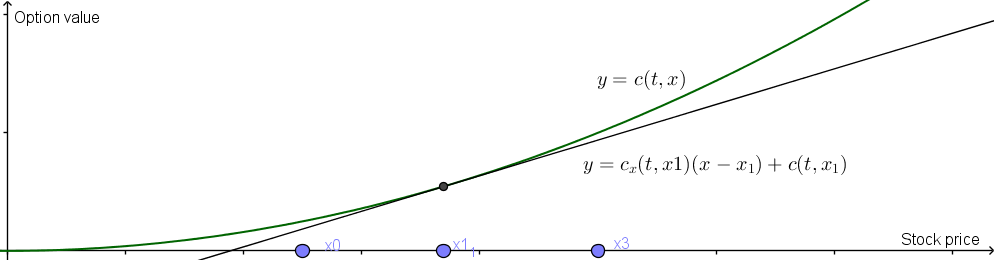
\includegraphics[width=1\textwidth]{../figures/test.png}
      \end{figure}
    \end{block}%
  
    \begin{block}{}
      \begin{itemize}
        \item Short Gamma
        \item Long Theta
      \end{itemize}
    \end{block}%
  
  

\end{frame}
%++++++++++++++++++++
\begin{frame}{Analysis and results: BSM}
  \begin{columns}[T] % align columns
  
    \begin{column}{.4\textwidth}
      \begin{itemize}
        \item Balancing frequency
        \item Negative effect on P\&L
        \begin{itemize}
          \item Short Gamma
        \end{itemize}
        \item Positive effect on P\&L
        \begin{itemize}
          \item Long Theta
        \end{itemize}
      \end{itemize}
    \end{column}%
  
  
  
  \begin{column}{.55\textwidth}
    \tiny
    \begin{tabular}{lllll}
      \hline
      \hline
       &  & 91 dbm & 182 dbm & 399 dbm \\ 
       \hdashline
      \multirow{3}{*}{140} & intraday & 0 & 0 & 0 \\ 
      & daily & 0 & 0 & 0 \\ 
      & weekly & 0 & 0 & 0 \\ 
       \hdashline
      \multirow{3}{*}{160} & intraday & 0 & 0 & 0 \\ 
      & daily & 0 & 0 & 0 \\ 
      & weekly & -0.001 & -0.001 & -0.003 \\ 
       \hdashline
      \multirow{3}{*}{186} & intraday & 0 & 0.001 & -0.001 \\ 
      & daily & -0.005 & -0.002 & -0.004 \\ 
      & weekly & -0.01 & -0.019 & -0.021 \\ 
       \hdashline
      \multirow{3}{*}{200} & intraday & 0.022 & 0.008 & -0.001 \\ 
      & daily & -0.002 & -0.005 & -0.006 \\ 
      & weekly & -0.007 & -0.052 & -0.037 \\ 
       \hdashline
      \multirow{3}{*}{230} & intraday & 0.02 & 0.042 & -0.007 \\ 
      & daily & 0.022 & -0.063 & -0.022 \\ 
      & weekly & 0.317 & -0.285 & -0.136 \\ 
       \hline
    \end{tabular}
  \end{column}%
  \end{columns}
\end{frame}
%++++++++++++++++++++
\begin{frame}{Analysis and results: BSM}
\begin{figure}[h]
  \centering
  % Created by tikzDevice version 0.11 on 2018-07-29 01:05:42
% !TEX encoding = UTF-8 Unicode
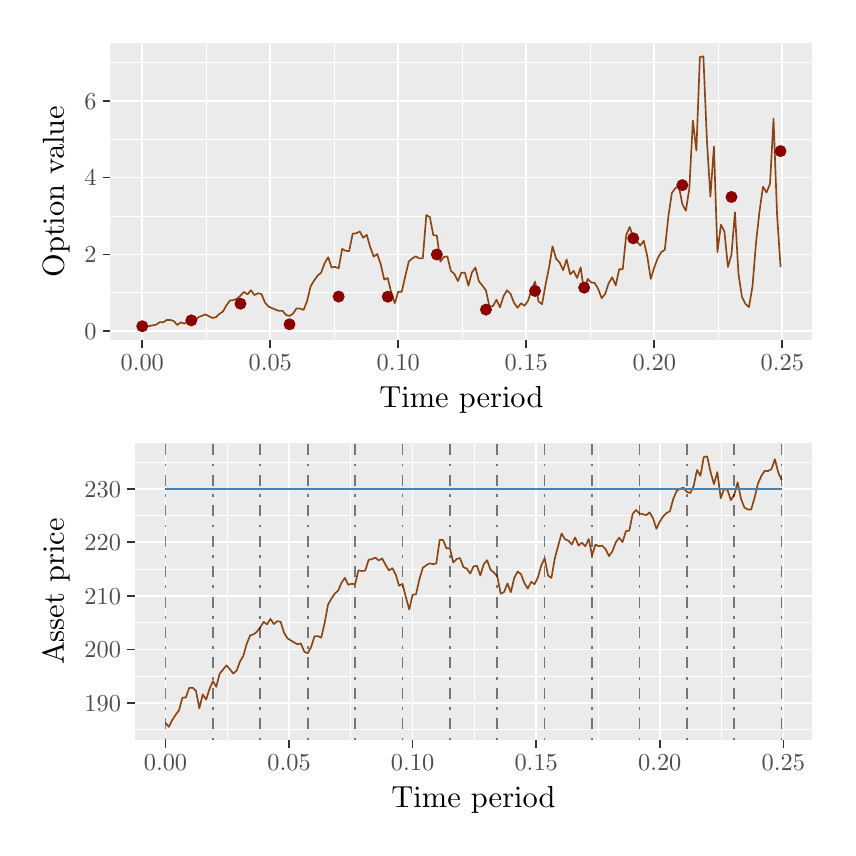
\begin{tikzpicture}[x=1pt,y=1pt]
\definecolor{fillColor}{RGB}{255,255,255}
\path[use as bounding box,fill=fillColor,fill opacity=0.00] (0,0) rectangle (289.08,289.08);
\begin{scope}
\path[clip] (  0.00,144.54) rectangle (289.08,289.08);
\definecolor{drawColor}{RGB}{255,255,255}
\definecolor{fillColor}{RGB}{255,255,255}

\path[draw=drawColor,line width= 0.6pt,line join=round,line cap=round,fill=fillColor] (  0.00,144.54) rectangle (289.08,289.08);
\end{scope}
\begin{scope}
\path[clip] ( 29.87,176.07) rectangle (283.58,283.58);
\definecolor{fillColor}{gray}{0.92}

\path[fill=fillColor] ( 29.87,176.07) rectangle (283.58,283.58);
\definecolor{drawColor}{RGB}{255,255,255}

\path[draw=drawColor,line width= 0.3pt,line join=round] ( 29.87,193.28) --
	(283.58,193.28);

\path[draw=drawColor,line width= 0.3pt,line join=round] ( 29.87,221.03) --
	(283.58,221.03);

\path[draw=drawColor,line width= 0.3pt,line join=round] ( 29.87,248.79) --
	(283.58,248.79);

\path[draw=drawColor,line width= 0.3pt,line join=round] ( 29.87,276.54) --
	(283.58,276.54);

\path[draw=drawColor,line width= 0.3pt,line join=round] ( 64.53,176.07) --
	( 64.53,283.58);

\path[draw=drawColor,line width= 0.3pt,line join=round] (110.79,176.07) --
	(110.79,283.58);

\path[draw=drawColor,line width= 0.3pt,line join=round] (157.04,176.07) --
	(157.04,283.58);

\path[draw=drawColor,line width= 0.3pt,line join=round] (203.30,176.07) --
	(203.30,283.58);

\path[draw=drawColor,line width= 0.3pt,line join=round] (249.55,176.07) --
	(249.55,283.58);

\path[draw=drawColor,line width= 0.6pt,line join=round] ( 29.87,179.41) --
	(283.58,179.41);

\path[draw=drawColor,line width= 0.6pt,line join=round] ( 29.87,207.16) --
	(283.58,207.16);

\path[draw=drawColor,line width= 0.6pt,line join=round] ( 29.87,234.91) --
	(283.58,234.91);

\path[draw=drawColor,line width= 0.6pt,line join=round] ( 29.87,262.66) --
	(283.58,262.66);

\path[draw=drawColor,line width= 0.6pt,line join=round] ( 41.40,176.07) --
	( 41.40,283.58);

\path[draw=drawColor,line width= 0.6pt,line join=round] ( 87.66,176.07) --
	( 87.66,283.58);

\path[draw=drawColor,line width= 0.6pt,line join=round] (133.91,176.07) --
	(133.91,283.58);

\path[draw=drawColor,line width= 0.6pt,line join=round] (180.17,176.07) --
	(180.17,283.58);

\path[draw=drawColor,line width= 0.6pt,line join=round] (226.43,176.07) --
	(226.43,283.58);

\path[draw=drawColor,line width= 0.6pt,line join=round] (272.68,176.07) --
	(272.68,283.58);
\definecolor{drawColor}{RGB}{139,69,19}

\path[draw=drawColor,line width= 0.6pt,line join=round] ( 41.40,181.19) --
	( 42.67,180.96) --
	( 43.94,181.27) --
	( 45.20,181.52) --
	( 46.47,181.77) --
	( 47.74,182.68) --
	( 49.00,182.63) --
	( 50.27,183.47) --
	( 51.54,183.44) --
	( 52.81,183.07) --
	( 54.07,181.63) --
	( 55.34,182.61) --
	( 56.61,182.14) --
	( 57.88,182.99) --
	( 59.14,183.74) --
	( 60.41,183.07) --
	( 61.68,184.48) --
	( 62.95,184.94) --
	( 64.21,185.47) --
	( 65.48,184.82) --
	( 66.75,184.18) --
	( 68.01,184.45) --
	( 69.28,185.65) --
	( 70.55,186.50) --
	( 71.82,188.73) --
	( 73.08,190.49) --
	( 74.35,190.62) --
	( 75.62,191.13) --
	( 76.89,192.21) --
	( 78.15,193.59) --
	( 79.42,192.69) --
	( 80.69,194.19) --
	( 81.95,192.45) --
	( 83.22,193.11) --
	( 84.49,192.79) --
	( 85.76,189.74) --
	( 87.02,188.32) --
	( 88.29,187.73) --
	( 89.56,187.19) --
	( 90.83,186.73) --
	( 92.09,186.76) --
	( 93.36,185.27) --
	( 94.63,184.92) --
	( 95.89,185.77) --
	( 97.16,187.66) --
	( 98.43,187.56) --
	( 99.70,187.10) --
	(100.96,190.26) --
	(102.23,195.62) --
	(103.50,197.68) --
	(104.77,199.50) --
	(106.03,200.51) --
	(107.30,203.98) --
	(108.57,206.12) --
	(109.83,202.41) --
	(111.10,202.65) --
	(112.37,202.13) --
	(113.64,209.15) --
	(114.90,208.44) --
	(116.17,208.36) --
	(117.44,214.61) --
	(118.71,214.78) --
	(119.97,215.45) --
	(121.24,213.16) --
	(122.51,214.21) --
	(123.77,209.83) --
	(125.04,206.34) --
	(126.31,207.29) --
	(127.58,203.57) --
	(128.84,198.08) --
	(130.11,198.59) --
	(131.38,193.33) --
	(132.65,189.50) --
	(133.91,193.66) --
	(135.18,193.64) --
	(136.45,199.32) --
	(137.72,204.62) --
	(138.98,205.69) --
	(140.25,206.45) --
	(141.52,205.70) --
	(142.78,205.73) --
	(144.05,221.38) --
	(145.32,220.64) --
	(146.59,214.06) --
	(147.85,213.98) --
	(149.12,204.56) --
	(150.39,206.24) --
	(151.66,206.42) --
	(152.92,201.16) --
	(154.19,200.08) --
	(155.46,197.49) --
	(156.72,200.57) --
	(157.99,200.50) --
	(159.26,195.84) --
	(160.53,200.64) --
	(161.79,202.38) --
	(163.06,197.40) --
	(164.33,195.87) --
	(165.60,194.12) --
	(166.86,188.28) --
	(168.13,188.48) --
	(169.40,190.78) --
	(170.66,188.02) --
	(171.93,192.04) --
	(173.20,194.18) --
	(174.47,192.90) --
	(175.73,189.69) --
	(177.00,187.87) --
	(178.27,189.50) --
	(179.54,188.59) --
	(180.80,190.38) --
	(182.07,194.42) --
	(183.34,197.35) --
	(184.60,190.14) --
	(185.87,189.17) --
	(187.14,196.23) --
	(188.41,202.50) --
	(189.67,210.06) --
	(190.94,205.60) --
	(192.21,204.23) --
	(193.48,201.45) --
	(194.74,205.31) --
	(196.01,199.97) --
	(197.28,201.20) --
	(198.54,198.63) --
	(199.81,202.49) --
	(201.08,193.50) --
	(202.35,198.30) --
	(203.61,197.02) --
	(204.88,196.84) --
	(206.15,194.69) --
	(207.42,191.33) --
	(208.68,192.87) --
	(209.95,196.76) --
	(211.22,198.88) --
	(212.49,195.98) --
	(213.75,201.81) --
	(215.02,201.78) --
	(216.29,214.16) --
	(217.55,217.07) --
	(218.82,213.16) --
	(220.09,211.84) --
	(221.36,210.34) --
	(222.62,212.08) --
	(223.89,206.43) --
	(225.16,198.29) --
	(226.43,202.49) --
	(227.69,205.82) --
	(228.96,207.99) --
	(230.23,208.79) --
	(231.49,220.62) --
	(232.76,229.32) --
	(234.03,231.09) --
	(235.30,231.75) --
	(236.56,225.34) --
	(237.83,222.91) --
	(239.10,231.05) --
	(240.37,255.49) --
	(241.63,244.67) --
	(242.90,278.48) --
	(244.17,278.69) --
	(245.43,248.47) --
	(246.70,228.01) --
	(247.97,246.11) --
	(249.24,207.96) --
	(250.50,217.88) --
	(251.77,215.36) --
	(253.04,202.59) --
	(254.31,207.06) --
	(255.57,222.38) --
	(256.84,200.14) --
	(258.11,191.74) --
	(259.37,189.21) --
	(260.64,188.12) --
	(261.91,195.61) --
	(263.18,211.30) --
	(264.44,222.75) --
	(265.71,231.60) --
	(266.98,229.52) --
	(268.25,232.69) --
	(269.51,256.19) --
	(270.78,221.72) --
	(272.05,202.60);
\definecolor{drawColor}{RGB}{139,0,0}
\definecolor{fillColor}{RGB}{139,0,0}

\path[draw=drawColor,line width= 0.4pt,line join=round,line cap=round,fill=fillColor] ( 41.40,181.19) circle (  1.96);

\path[draw=drawColor,line width= 0.4pt,line join=round,line cap=round,fill=fillColor] ( 59.14,183.31) circle (  1.96);

\path[draw=drawColor,line width= 0.4pt,line join=round,line cap=round,fill=fillColor] ( 76.89,189.33) circle (  1.96);

\path[draw=drawColor,line width= 0.4pt,line join=round,line cap=round,fill=fillColor] ( 94.63,181.89) circle (  1.96);

\path[draw=drawColor,line width= 0.4pt,line join=round,line cap=round,fill=fillColor] (112.37,191.91) circle (  1.96);

\path[draw=drawColor,line width= 0.4pt,line join=round,line cap=round,fill=fillColor] (130.11,191.87) circle (  1.96);

\path[draw=drawColor,line width= 0.4pt,line join=round,line cap=round,fill=fillColor] (147.85,207.11) circle (  1.96);

\path[draw=drawColor,line width= 0.4pt,line join=round,line cap=round,fill=fillColor] (165.60,187.19) circle (  1.96);

\path[draw=drawColor,line width= 0.4pt,line join=round,line cap=round,fill=fillColor] (183.34,193.94) circle (  1.96);

\path[draw=drawColor,line width= 0.4pt,line join=round,line cap=round,fill=fillColor] (201.08,195.14) circle (  1.96);

\path[draw=drawColor,line width= 0.4pt,line join=round,line cap=round,fill=fillColor] (218.82,212.96) circle (  1.96);

\path[draw=drawColor,line width= 0.4pt,line join=round,line cap=round,fill=fillColor] (236.56,232.18) circle (  1.96);

\path[draw=drawColor,line width= 0.4pt,line join=round,line cap=round,fill=fillColor] (254.31,227.90) circle (  1.96);

\path[draw=drawColor,line width= 0.4pt,line join=round,line cap=round,fill=fillColor] (272.05,244.47) circle (  1.96);
\end{scope}
\begin{scope}
\path[clip] (  0.00,  0.00) rectangle (289.08,289.08);
\definecolor{drawColor}{gray}{0.30}

\node[text=drawColor,anchor=base east,inner sep=0pt, outer sep=0pt, scale=  0.88] at ( 24.92,176.37) {0};

\node[text=drawColor,anchor=base east,inner sep=0pt, outer sep=0pt, scale=  0.88] at ( 24.92,204.13) {2};

\node[text=drawColor,anchor=base east,inner sep=0pt, outer sep=0pt, scale=  0.88] at ( 24.92,231.88) {4};

\node[text=drawColor,anchor=base east,inner sep=0pt, outer sep=0pt, scale=  0.88] at ( 24.92,259.63) {6};
\end{scope}
\begin{scope}
\path[clip] (  0.00,  0.00) rectangle (289.08,289.08);
\definecolor{drawColor}{gray}{0.20}

\path[draw=drawColor,line width= 0.6pt,line join=round] ( 27.12,179.41) --
	( 29.87,179.41);

\path[draw=drawColor,line width= 0.6pt,line join=round] ( 27.12,207.16) --
	( 29.87,207.16);

\path[draw=drawColor,line width= 0.6pt,line join=round] ( 27.12,234.91) --
	( 29.87,234.91);

\path[draw=drawColor,line width= 0.6pt,line join=round] ( 27.12,262.66) --
	( 29.87,262.66);
\end{scope}
\begin{scope}
\path[clip] (  0.00,  0.00) rectangle (289.08,289.08);
\definecolor{drawColor}{gray}{0.20}

\path[draw=drawColor,line width= 0.6pt,line join=round] ( 41.40,173.32) --
	( 41.40,176.07);

\path[draw=drawColor,line width= 0.6pt,line join=round] ( 87.66,173.32) --
	( 87.66,176.07);

\path[draw=drawColor,line width= 0.6pt,line join=round] (133.91,173.32) --
	(133.91,176.07);

\path[draw=drawColor,line width= 0.6pt,line join=round] (180.17,173.32) --
	(180.17,176.07);

\path[draw=drawColor,line width= 0.6pt,line join=round] (226.43,173.32) --
	(226.43,176.07);

\path[draw=drawColor,line width= 0.6pt,line join=round] (272.68,173.32) --
	(272.68,176.07);
\end{scope}
\begin{scope}
\path[clip] (  0.00,  0.00) rectangle (289.08,289.08);
\definecolor{drawColor}{gray}{0.30}

\node[text=drawColor,anchor=base,inner sep=0pt, outer sep=0pt, scale=  0.88] at ( 41.40,165.06) {0.00};

\node[text=drawColor,anchor=base,inner sep=0pt, outer sep=0pt, scale=  0.88] at ( 87.66,165.06) {0.05};

\node[text=drawColor,anchor=base,inner sep=0pt, outer sep=0pt, scale=  0.88] at (133.91,165.06) {0.10};

\node[text=drawColor,anchor=base,inner sep=0pt, outer sep=0pt, scale=  0.88] at (180.17,165.06) {0.15};

\node[text=drawColor,anchor=base,inner sep=0pt, outer sep=0pt, scale=  0.88] at (226.43,165.06) {0.20};

\node[text=drawColor,anchor=base,inner sep=0pt, outer sep=0pt, scale=  0.88] at (272.68,165.06) {0.25};
\end{scope}
\begin{scope}
\path[clip] (  0.00,  0.00) rectangle (289.08,289.08);
\definecolor{drawColor}{RGB}{0,0,0}

\node[text=drawColor,anchor=base,inner sep=0pt, outer sep=0pt, scale=  1.10] at (156.72,151.98) {Time period};
\end{scope}
\begin{scope}
\path[clip] (  0.00,  0.00) rectangle (289.08,289.08);
\definecolor{drawColor}{RGB}{0,0,0}

\node[text=drawColor,rotate= 90.00,anchor=base,inner sep=0pt, outer sep=0pt, scale=  1.10] at ( 13.08,229.83) {Option value};
\end{scope}
\begin{scope}
\path[clip] (  0.00,  0.00) rectangle (289.08,144.54);
\definecolor{drawColor}{RGB}{255,255,255}
\definecolor{fillColor}{RGB}{255,255,255}

\path[draw=drawColor,line width= 0.6pt,line join=round,line cap=round,fill=fillColor] (  0.00,  0.00) rectangle (289.08,144.54);
\end{scope}
\begin{scope}
\path[clip] ( 38.67, 31.53) rectangle (283.58,139.04);
\definecolor{fillColor}{gray}{0.92}

\path[fill=fillColor] ( 38.67, 31.53) rectangle (283.58,139.04);
\definecolor{drawColor}{RGB}{255,255,255}

\path[draw=drawColor,line width= 0.3pt,line join=round] ( 38.67, 35.34) --
	(283.58, 35.34);

\path[draw=drawColor,line width= 0.3pt,line join=round] ( 38.67, 54.70) --
	(283.58, 54.70);

\path[draw=drawColor,line width= 0.3pt,line join=round] ( 38.67, 74.06) --
	(283.58, 74.06);

\path[draw=drawColor,line width= 0.3pt,line join=round] ( 38.67, 93.43) --
	(283.58, 93.43);

\path[draw=drawColor,line width= 0.3pt,line join=round] ( 38.67,112.79) --
	(283.58,112.79);

\path[draw=drawColor,line width= 0.3pt,line join=round] ( 38.67,132.15) --
	(283.58,132.15);

\path[draw=drawColor,line width= 0.3pt,line join=round] ( 72.13, 31.53) --
	( 72.13,139.04);

\path[draw=drawColor,line width= 0.3pt,line join=round] (116.78, 31.53) --
	(116.78,139.04);

\path[draw=drawColor,line width= 0.3pt,line join=round] (161.43, 31.53) --
	(161.43,139.04);

\path[draw=drawColor,line width= 0.3pt,line join=round] (206.08, 31.53) --
	(206.08,139.04);

\path[draw=drawColor,line width= 0.3pt,line join=round] (250.73, 31.53) --
	(250.73,139.04);

\path[draw=drawColor,line width= 0.6pt,line join=round] ( 38.67, 45.02) --
	(283.58, 45.02);

\path[draw=drawColor,line width= 0.6pt,line join=round] ( 38.67, 64.38) --
	(283.58, 64.38);

\path[draw=drawColor,line width= 0.6pt,line join=round] ( 38.67, 83.75) --
	(283.58, 83.75);

\path[draw=drawColor,line width= 0.6pt,line join=round] ( 38.67,103.11) --
	(283.58,103.11);

\path[draw=drawColor,line width= 0.6pt,line join=round] ( 38.67,122.47) --
	(283.58,122.47);

\path[draw=drawColor,line width= 0.6pt,line join=round] ( 49.80, 31.53) --
	( 49.80,139.04);

\path[draw=drawColor,line width= 0.6pt,line join=round] ( 94.45, 31.53) --
	( 94.45,139.04);

\path[draw=drawColor,line width= 0.6pt,line join=round] (139.10, 31.53) --
	(139.10,139.04);

\path[draw=drawColor,line width= 0.6pt,line join=round] (183.76, 31.53) --
	(183.76,139.04);

\path[draw=drawColor,line width= 0.6pt,line join=round] (228.41, 31.53) --
	(228.41,139.04);

\path[draw=drawColor,line width= 0.6pt,line join=round] (273.06, 31.53) --
	(273.06,139.04);
\definecolor{drawColor}{RGB}{139,69,19}

\path[draw=drawColor,line width= 0.6pt,line join=round] ( 49.80, 37.88) --
	( 51.02, 36.42) --
	( 52.25, 38.92) --
	( 53.47, 40.78) --
	( 54.69, 42.43) --
	( 55.92, 47.00) --
	( 57.14, 47.02) --
	( 58.36, 50.46) --
	( 59.59, 50.58) --
	( 60.81, 49.47) --
	( 62.03, 43.14) --
	( 63.26, 48.13) --
	( 64.48, 46.27) --
	( 65.70, 50.11) --
	( 66.93, 52.96) --
	( 68.15, 50.89) --
	( 69.37, 55.64) --
	( 70.60, 57.12) --
	( 71.82, 58.66) --
	( 73.04, 57.27) --
	( 74.27, 55.72) --
	( 75.49, 56.70) --
	( 76.71, 60.01) --
	( 77.94, 62.12) --
	( 79.16, 66.49) --
	( 80.38, 69.46) --
	( 81.61, 69.86) --
	( 82.83, 70.79) --
	( 84.05, 72.44) --
	( 85.28, 74.36) --
	( 86.50, 73.46) --
	( 87.72, 75.45) --
	( 88.95, 73.58) --
	( 90.17, 74.61) --
	( 91.39, 74.43) --
	( 92.62, 70.50) --
	( 93.84, 68.47) --
	( 95.06, 67.66) --
	( 96.29, 66.91) --
	( 97.51, 66.26) --
	( 98.73, 66.56) --
	( 99.96, 63.60) --
	(101.18, 62.99) --
	(102.40, 65.21) --
	(103.63, 69.16) --
	(104.85, 69.23) --
	(106.07, 68.63) --
	(107.30, 73.95) --
	(108.52, 80.54) --
	(109.74, 82.76) --
	(110.97, 84.58) --
	(112.19, 85.64) --
	(113.41, 88.53) --
	(114.64, 90.25) --
	(115.86, 87.76) --
	(117.08, 88.14) --
	(118.31, 87.95) --
	(119.53, 93.00) --
	(120.75, 92.75) --
	(121.98, 92.89) --
	(123.20, 96.77) --
	(124.42, 97.05) --
	(125.65, 97.60) --
	(126.87, 96.53) --
	(128.09, 97.29) --
	(129.32, 94.97) --
	(130.54, 92.97) --
	(131.76, 93.78) --
	(132.99, 91.49) --
	(134.21, 87.41) --
	(135.43, 88.07) --
	(136.66, 83.31) --
	(137.88, 78.89) --
	(139.10, 84.14) --
	(140.33, 84.35) --
	(141.55, 89.79) --
	(142.77, 93.89) --
	(144.00, 94.81) --
	(145.22, 95.51) --
	(146.44, 95.24) --
	(147.67, 95.48) --
	(148.89,104.06) --
	(150.11,103.91) --
	(151.34,100.89) --
	(152.56,101.05) --
	(153.78, 95.80) --
	(155.01, 97.09) --
	(156.23, 97.42) --
	(157.45, 94.15) --
	(158.68, 93.59) --
	(159.90, 91.80) --
	(161.12, 94.42) --
	(162.35, 94.61) --
	(163.57, 91.14) --
	(164.79, 95.18) --
	(166.02, 96.64) --
	(167.24, 93.21) --
	(168.46, 92.19) --
	(169.69, 90.87) --
	(170.91, 84.55) --
	(172.13, 85.12) --
	(173.36, 88.26) --
	(174.58, 85.07) --
	(175.80, 90.19) --
	(177.03, 92.55) --
	(178.25, 91.62) --
	(179.47, 88.45) --
	(180.70, 86.39) --
	(181.92, 88.82) --
	(183.14, 87.98) --
	(184.37, 90.45) --
	(185.59, 94.71) --
	(186.81, 97.36) --
	(188.04, 91.09) --
	(189.26, 90.28) --
	(190.48, 97.33) --
	(191.71,101.92) --
	(192.93,106.30) --
	(194.15,104.22) --
	(195.38,103.72) --
	(196.60,102.34) --
	(197.82,104.84) --
	(199.05,101.95) --
	(200.27,103.00) --
	(201.49,101.64) --
	(202.72,104.33) --
	(203.94, 98.41) --
	(205.16,102.30) --
	(206.39,101.72) --
	(207.61,101.90) --
	(208.83,100.64) --
	(210.06, 98.14) --
	(211.28, 99.84) --
	(212.50,103.09) --
	(213.73,104.79) --
	(214.95,103.20) --
	(216.17,107.11) --
	(217.40,107.40) --
	(218.62,113.40) --
	(219.84,114.77) --
	(221.07,113.53) --
	(222.29,113.27) --
	(223.51,112.94) --
	(224.74,113.92) --
	(225.96,111.83) --
	(227.18,108.01) --
	(228.41,110.59) --
	(229.63,112.47) --
	(230.85,113.72) --
	(232.08,114.35) --
	(233.30,118.87) --
	(234.52,121.71) --
	(235.75,122.44) --
	(236.97,122.86) --
	(238.19,121.34) --
	(239.42,120.91) --
	(240.64,123.40) --
	(241.86,129.24) --
	(243.09,127.12) --
	(244.31,133.97) --
	(245.53,134.15) --
	(246.76,128.56) --
	(247.98,124.16) --
	(249.20,128.48) --
	(250.43,119.05) --
	(251.65,122.39) --
	(252.87,122.02) --
	(254.10,118.34) --
	(255.32,120.28) --
	(256.54,124.79) --
	(257.77,118.79) --
	(258.99,115.71) --
	(260.21,114.94) --
	(261.44,114.97) --
	(262.66,119.20) --
	(263.88,124.29) --
	(265.11,127.08) --
	(266.33,128.96) --
	(267.55,128.86) --
	(268.78,129.59) --
	(270.00,133.14) --
	(271.22,128.31) --
	(272.45,125.70);
\definecolor{drawColor}{RGB}{70,130,180}

\path[draw=drawColor,line width= 0.6pt,line join=round] ( 49.80,122.47) --
	( 51.02,122.47) --
	( 52.25,122.47) --
	( 53.47,122.47) --
	( 54.69,122.47) --
	( 55.92,122.47) --
	( 57.14,122.47) --
	( 58.36,122.47) --
	( 59.59,122.47) --
	( 60.81,122.47) --
	( 62.03,122.47) --
	( 63.26,122.47) --
	( 64.48,122.47) --
	( 65.70,122.47) --
	( 66.93,122.47) --
	( 68.15,122.47) --
	( 69.37,122.47) --
	( 70.60,122.47) --
	( 71.82,122.47) --
	( 73.04,122.47) --
	( 74.27,122.47) --
	( 75.49,122.47) --
	( 76.71,122.47) --
	( 77.94,122.47) --
	( 79.16,122.47) --
	( 80.38,122.47) --
	( 81.61,122.47) --
	( 82.83,122.47) --
	( 84.05,122.47) --
	( 85.28,122.47) --
	( 86.50,122.47) --
	( 87.72,122.47) --
	( 88.95,122.47) --
	( 90.17,122.47) --
	( 91.39,122.47) --
	( 92.62,122.47) --
	( 93.84,122.47) --
	( 95.06,122.47) --
	( 96.29,122.47) --
	( 97.51,122.47) --
	( 98.73,122.47) --
	( 99.96,122.47) --
	(101.18,122.47) --
	(102.40,122.47) --
	(103.63,122.47) --
	(104.85,122.47) --
	(106.07,122.47) --
	(107.30,122.47) --
	(108.52,122.47) --
	(109.74,122.47) --
	(110.97,122.47) --
	(112.19,122.47) --
	(113.41,122.47) --
	(114.64,122.47) --
	(115.86,122.47) --
	(117.08,122.47) --
	(118.31,122.47) --
	(119.53,122.47) --
	(120.75,122.47) --
	(121.98,122.47) --
	(123.20,122.47) --
	(124.42,122.47) --
	(125.65,122.47) --
	(126.87,122.47) --
	(128.09,122.47) --
	(129.32,122.47) --
	(130.54,122.47) --
	(131.76,122.47) --
	(132.99,122.47) --
	(134.21,122.47) --
	(135.43,122.47) --
	(136.66,122.47) --
	(137.88,122.47) --
	(139.10,122.47) --
	(140.33,122.47) --
	(141.55,122.47) --
	(142.77,122.47) --
	(144.00,122.47) --
	(145.22,122.47) --
	(146.44,122.47) --
	(147.67,122.47) --
	(148.89,122.47) --
	(150.11,122.47) --
	(151.34,122.47) --
	(152.56,122.47) --
	(153.78,122.47) --
	(155.01,122.47) --
	(156.23,122.47) --
	(157.45,122.47) --
	(158.68,122.47) --
	(159.90,122.47) --
	(161.12,122.47) --
	(162.35,122.47) --
	(163.57,122.47) --
	(164.79,122.47) --
	(166.02,122.47) --
	(167.24,122.47) --
	(168.46,122.47) --
	(169.69,122.47) --
	(170.91,122.47) --
	(172.13,122.47) --
	(173.36,122.47) --
	(174.58,122.47) --
	(175.80,122.47) --
	(177.03,122.47) --
	(178.25,122.47) --
	(179.47,122.47) --
	(180.70,122.47) --
	(181.92,122.47) --
	(183.14,122.47) --
	(184.37,122.47) --
	(185.59,122.47) --
	(186.81,122.47) --
	(188.04,122.47) --
	(189.26,122.47) --
	(190.48,122.47) --
	(191.71,122.47) --
	(192.93,122.47) --
	(194.15,122.47) --
	(195.38,122.47) --
	(196.60,122.47) --
	(197.82,122.47) --
	(199.05,122.47) --
	(200.27,122.47) --
	(201.49,122.47) --
	(202.72,122.47) --
	(203.94,122.47) --
	(205.16,122.47) --
	(206.39,122.47) --
	(207.61,122.47) --
	(208.83,122.47) --
	(210.06,122.47) --
	(211.28,122.47) --
	(212.50,122.47) --
	(213.73,122.47) --
	(214.95,122.47) --
	(216.17,122.47) --
	(217.40,122.47) --
	(218.62,122.47) --
	(219.84,122.47) --
	(221.07,122.47) --
	(222.29,122.47) --
	(223.51,122.47) --
	(224.74,122.47) --
	(225.96,122.47) --
	(227.18,122.47) --
	(228.41,122.47) --
	(229.63,122.47) --
	(230.85,122.47) --
	(232.08,122.47) --
	(233.30,122.47) --
	(234.52,122.47) --
	(235.75,122.47) --
	(236.97,122.47) --
	(238.19,122.47) --
	(239.42,122.47) --
	(240.64,122.47) --
	(241.86,122.47) --
	(243.09,122.47) --
	(244.31,122.47) --
	(245.53,122.47) --
	(246.76,122.47) --
	(247.98,122.47) --
	(249.20,122.47) --
	(250.43,122.47) --
	(251.65,122.47) --
	(252.87,122.47) --
	(254.10,122.47) --
	(255.32,122.47) --
	(256.54,122.47) --
	(257.77,122.47) --
	(258.99,122.47) --
	(260.21,122.47) --
	(261.44,122.47) --
	(262.66,122.47) --
	(263.88,122.47) --
	(265.11,122.47) --
	(266.33,122.47) --
	(267.55,122.47) --
	(268.78,122.47) --
	(270.00,122.47) --
	(271.22,122.47) --
	(272.45,122.47);
\definecolor{drawColor}{RGB}{0,0,0}

\path[draw=drawColor,draw opacity=0.50,line width= 0.6pt,dash pattern=on 1pt off 3pt on 4pt off 3pt ,line join=round] ( 49.80, 31.53) -- ( 49.80,139.04);

\path[draw=drawColor,draw opacity=0.50,line width= 0.6pt,dash pattern=on 1pt off 3pt on 4pt off 3pt ,line join=round] ( 66.93, 31.53) -- ( 66.93,139.04);

\path[draw=drawColor,draw opacity=0.50,line width= 0.6pt,dash pattern=on 1pt off 3pt on 4pt off 3pt ,line join=round] ( 84.05, 31.53) -- ( 84.05,139.04);

\path[draw=drawColor,draw opacity=0.50,line width= 0.6pt,dash pattern=on 1pt off 3pt on 4pt off 3pt ,line join=round] (101.18, 31.53) -- (101.18,139.04);

\path[draw=drawColor,draw opacity=0.50,line width= 0.6pt,dash pattern=on 1pt off 3pt on 4pt off 3pt ,line join=round] (118.31, 31.53) -- (118.31,139.04);

\path[draw=drawColor,draw opacity=0.50,line width= 0.6pt,dash pattern=on 1pt off 3pt on 4pt off 3pt ,line join=round] (135.43, 31.53) -- (135.43,139.04);

\path[draw=drawColor,draw opacity=0.50,line width= 0.6pt,dash pattern=on 1pt off 3pt on 4pt off 3pt ,line join=round] (152.56, 31.53) -- (152.56,139.04);

\path[draw=drawColor,draw opacity=0.50,line width= 0.6pt,dash pattern=on 1pt off 3pt on 4pt off 3pt ,line join=round] (169.69, 31.53) -- (169.69,139.04);

\path[draw=drawColor,draw opacity=0.50,line width= 0.6pt,dash pattern=on 1pt off 3pt on 4pt off 3pt ,line join=round] (186.81, 31.53) -- (186.81,139.04);

\path[draw=drawColor,draw opacity=0.50,line width= 0.6pt,dash pattern=on 1pt off 3pt on 4pt off 3pt ,line join=round] (203.94, 31.53) -- (203.94,139.04);

\path[draw=drawColor,draw opacity=0.50,line width= 0.6pt,dash pattern=on 1pt off 3pt on 4pt off 3pt ,line join=round] (221.07, 31.53) -- (221.07,139.04);

\path[draw=drawColor,draw opacity=0.50,line width= 0.6pt,dash pattern=on 1pt off 3pt on 4pt off 3pt ,line join=round] (238.19, 31.53) -- (238.19,139.04);

\path[draw=drawColor,draw opacity=0.50,line width= 0.6pt,dash pattern=on 1pt off 3pt on 4pt off 3pt ,line join=round] (255.32, 31.53) -- (255.32,139.04);

\path[draw=drawColor,draw opacity=0.50,line width= 0.6pt,dash pattern=on 1pt off 3pt on 4pt off 3pt ,line join=round] (272.45, 31.53) -- (272.45,139.04);
\end{scope}
\begin{scope}
\path[clip] (  0.00,  0.00) rectangle (289.08,289.08);
\definecolor{drawColor}{gray}{0.30}

\node[text=drawColor,anchor=base east,inner sep=0pt, outer sep=0pt, scale=  0.88] at ( 33.72, 41.99) {190};

\node[text=drawColor,anchor=base east,inner sep=0pt, outer sep=0pt, scale=  0.88] at ( 33.72, 61.35) {200};

\node[text=drawColor,anchor=base east,inner sep=0pt, outer sep=0pt, scale=  0.88] at ( 33.72, 80.72) {210};

\node[text=drawColor,anchor=base east,inner sep=0pt, outer sep=0pt, scale=  0.88] at ( 33.72,100.08) {220};

\node[text=drawColor,anchor=base east,inner sep=0pt, outer sep=0pt, scale=  0.88] at ( 33.72,119.44) {230};
\end{scope}
\begin{scope}
\path[clip] (  0.00,  0.00) rectangle (289.08,289.08);
\definecolor{drawColor}{gray}{0.20}

\path[draw=drawColor,line width= 0.6pt,line join=round] ( 35.92, 45.02) --
	( 38.67, 45.02);

\path[draw=drawColor,line width= 0.6pt,line join=round] ( 35.92, 64.38) --
	( 38.67, 64.38);

\path[draw=drawColor,line width= 0.6pt,line join=round] ( 35.92, 83.75) --
	( 38.67, 83.75);

\path[draw=drawColor,line width= 0.6pt,line join=round] ( 35.92,103.11) --
	( 38.67,103.11);

\path[draw=drawColor,line width= 0.6pt,line join=round] ( 35.92,122.47) --
	( 38.67,122.47);
\end{scope}
\begin{scope}
\path[clip] (  0.00,  0.00) rectangle (289.08,289.08);
\definecolor{drawColor}{gray}{0.20}

\path[draw=drawColor,line width= 0.6pt,line join=round] ( 49.80, 28.78) --
	( 49.80, 31.53);

\path[draw=drawColor,line width= 0.6pt,line join=round] ( 94.45, 28.78) --
	( 94.45, 31.53);

\path[draw=drawColor,line width= 0.6pt,line join=round] (139.10, 28.78) --
	(139.10, 31.53);

\path[draw=drawColor,line width= 0.6pt,line join=round] (183.76, 28.78) --
	(183.76, 31.53);

\path[draw=drawColor,line width= 0.6pt,line join=round] (228.41, 28.78) --
	(228.41, 31.53);

\path[draw=drawColor,line width= 0.6pt,line join=round] (273.06, 28.78) --
	(273.06, 31.53);
\end{scope}
\begin{scope}
\path[clip] (  0.00,  0.00) rectangle (289.08,289.08);
\definecolor{drawColor}{gray}{0.30}

\node[text=drawColor,anchor=base,inner sep=0pt, outer sep=0pt, scale=  0.88] at ( 49.80, 20.52) {0.00};

\node[text=drawColor,anchor=base,inner sep=0pt, outer sep=0pt, scale=  0.88] at ( 94.45, 20.52) {0.05};

\node[text=drawColor,anchor=base,inner sep=0pt, outer sep=0pt, scale=  0.88] at (139.10, 20.52) {0.10};

\node[text=drawColor,anchor=base,inner sep=0pt, outer sep=0pt, scale=  0.88] at (183.76, 20.52) {0.15};

\node[text=drawColor,anchor=base,inner sep=0pt, outer sep=0pt, scale=  0.88] at (228.41, 20.52) {0.20};

\node[text=drawColor,anchor=base,inner sep=0pt, outer sep=0pt, scale=  0.88] at (273.06, 20.52) {0.25};
\end{scope}
\begin{scope}
\path[clip] (  0.00,  0.00) rectangle (289.08,289.08);
\definecolor{drawColor}{RGB}{0,0,0}

\node[text=drawColor,anchor=base,inner sep=0pt, outer sep=0pt, scale=  1.10] at (161.12,  7.44) {Time period};
\end{scope}
\begin{scope}
\path[clip] (  0.00,  0.00) rectangle (289.08,289.08);
\definecolor{drawColor}{RGB}{0,0,0}

\node[text=drawColor,rotate= 90.00,anchor=base,inner sep=0pt, outer sep=0pt, scale=  1.10] at ( 13.08, 85.29) {Asset price};
\end{scope}
\end{tikzpicture}

\end{figure}
\end{frame}
% -----------------------------------------------------------------------------













\subsection{Analysis and results: Merton}
% ----------------------------------------------------------------------------- 
\begin{frame}{Analysis and results: Merton}

\begin{table}[h]
\small
\centering
\begin{tabular}{llllllll}
  \hline
  \hline
 Strikes & frequency  &\multicolumn{2}{c}{91 dbm} & \multicolumn{2}{c}{182 dbm} & \multicolumn{2}{c}{399 dbm} \\ 
   &  & $\Delta_{mrt}$ & $\Delta_{bsm}$ & $\Delta_{mrt}$ & $\Delta_{bsm}$ & $\Delta_{mrt}$ & $\Delta_{bsm}$ \\ 
   \hdashline
  \multirow{3}{*}{140} & intraday & 0.004 & 0.006 & 0.011 & 0.012 & 0.01 & 0.021 \\ 
  & daily & 0.002 & 0.006 & 0.008 & 0.012 & 0.016 & 0.021 \\ 
  & weekly & 0.004 & 0.006 & 0.006 & 0.011 & 0.007 & 0.021 \\ 
   \hdashline
  \multirow{3}{*}{160} & intraday & 0.011 & 0.018 & 0.021 & 0.029 & 0.025 & 0.042 \\ 
  & daily & 0.016 & 0.018 & 0.022 & 0.029 & 0.019 & 0.042 \\ 
  & weekly & 0.013 & 0.016 & 0.018 & 0.026 & 0.018 & 0.04 \\ 
   \hdashline
  \multirow{3}{*}{186} & intraday & 0.036 & 0.021 & 0.078 & 0.055 & 0.079 & 0.074 \\ 
  & daily & 0.039 & 0.022 & 0.072 & 0.055 & 0.068 & 0.074 \\ 
  & weekly & 0.014 & -0.008 & 0.055 & 0.037 & 0.057 & 0.061 \\ 
   \hdashline
  \multirow{3}{*}{200} & intraday & 0.072 & -0.002 & 0.139 & 0.061 & 0.13 & 0.086 \\ 
  & daily & 0.06 & -0.013 & 0.131 & 0.057 & 0.115 & 0.085 \\ 
  & weekly & -0.02 & -0.1 & 0.083 & 0.005 & 0.085 & 0.053 \\ 
   \hdashline
  \multirow{3}{*}{230} & intraday & 0.955 & 0.331 & 0.444 & -0.061 & 0.301 & 0.063 \\ 
  & daily & 1.098 & 0.466 & 0.409 & -0.091 & 0.261 & 0.054 \\ 
  & weekly & -0.741 & -1.335 & 0.085 & -0.438 & 0.174 & -0.088 \\ 
   \hline
\end{tabular}
\caption{Hedging with MJD: Relative P\&L} 
\label{t:analysis:merton:pl}
\end{table}
 
\end{frame}
% -----------------------------------------------------------------------------


\subsection{Analysis and results: Heston}
% ----------------------------------------------------------------------------- 
\begin{frame}{Analysis and results: Heston}

\begin{table}[ht]
\small
\centering
\begin{tabular}{llllllll}
  \hline
  \hline
Strikes & frequency  &\multicolumn{2}{c}{91 dbm} & \multicolumn{2}{c}{182 dbm} & \multicolumn{2}{c}{399 dbm} \\ 
   &  & $\Delta_{hsv}$ & $\Delta_{bsm}$ & $\Delta_{hsv}$ & $\Delta_{bsm}$ & $\Delta_{hsv}$ & $\Delta_{bsm}$ \\ 
   \hdashline
  \multirow{3}{*}{140} & intraday & 0 & 0.002 & 0.011 & 0.011 & 0.009 & 0.038 \\ 
  & daily & -0.001 & 0.002 & 0.01 & 0.011 & 0.009 & 0.038 \\ 
  & weekly & 0.001 & 0.002 & 0 & 0.011 & 0.008 & 0.038 \\ 
  \hdashline
  \multirow{3}{*}{160} & intraday & 0.009 & 0.028 & 0.023 & 0.073 & 0.042 & 0.143 \\ 
  & daily & 0.008 & 0.028 & 0.025 & 0.072 & 0.036 & 0.143 \\ 
  & weekly & 0.008 & 0.028 & 0.019 & 0.073 & 0.036 & 0.143 \\ 
  \hdashline
  \multirow{3}{*}{186} & intraday & 0.158 & 0.252 & 0.159 & 0.392 & 0.153 & 0.524 \\ 
  & daily & 0.15 & 0.245 & 0.195 & 0.391 & 0.156 & 0.522 \\ 
  & weekly & 0.117 & 0.241 & 0.158 & 0.378 & 0.139 & 0.519 \\ 
  \hdashline 
  \multirow{3}{*}{200} & intraday & 0.459 & -0.298 & 0.43 & 0.146 & 0.279 & 0.546 \\ 
  & daily & 0.433 & -0.361 & 0.42 & 0.126 & 0.255 & 0.544 \\ 
  & weekly & 0.268 & -0.659 & 0.369 & 0.005 & 0.246 & 0.498 \\ 
  \hdashline 
  \multirow{3}{*}{230} & intraday & 2.136 & -0.527 & 1.884 & -2.452 & 1.01 & -0.235 \\ 
  & daily & 1.948 & -1.197 & 1.893 & -2.655 & 0.989 & -0.224 \\ 
  & weekly & 1.407 & -2.152 & 1.547 & -2.402 & 0.917 & -0.353 \\ 
   \hline
\end{tabular}
\caption{Hedging with HSV: Relative P\&L} 
\label{t:analysis:heston:pl}
\end{table}
 
\end{frame}
% -----------------------------------------------------------------------------




 
\end{document}
